\documentclass[twoside]{book}

% Packages required by doxygen
\usepackage{fixltx2e}
\usepackage{calc}
\usepackage{doxygen}
\usepackage{graphicx}
\usepackage[utf8]{inputenc}
\usepackage{makeidx}
\usepackage{multicol}
\usepackage{multirow}
\PassOptionsToPackage{warn}{textcomp}
\usepackage{textcomp}
\usepackage[nointegrals]{wasysym}
\usepackage[table]{xcolor}

% Font selection
\usepackage[T1]{fontenc}
\usepackage{mathptmx}
\usepackage[scaled=.90]{helvet}
\usepackage{courier}
\usepackage{amssymb}
\usepackage{sectsty}
\renewcommand{\familydefault}{\sfdefault}
\allsectionsfont{%
  \fontseries{bc}\selectfont%
  \color{darkgray}%
}
\renewcommand{\DoxyLabelFont}{%
  \fontseries{bc}\selectfont%
  \color{darkgray}%
}
\newcommand{\+}{\discretionary{\mbox{\scriptsize$\hookleftarrow$}}{}{}}

% Page & text layout
\usepackage{geometry}
\geometry{%
  a4paper,%
  top=2.5cm,%
  bottom=2.5cm,%
  left=2.5cm,%
  right=2.5cm%
}
\tolerance=750
\hfuzz=15pt
\hbadness=750
\setlength{\emergencystretch}{15pt}
\setlength{\parindent}{0cm}
\setlength{\parskip}{0.2cm}
\makeatletter
\renewcommand{\paragraph}{%
  \@startsection{paragraph}{4}{0ex}{-1.0ex}{1.0ex}{%
    \normalfont\normalsize\bfseries\SS@parafont%
  }%
}
\renewcommand{\subparagraph}{%
  \@startsection{subparagraph}{5}{0ex}{-1.0ex}{1.0ex}{%
    \normalfont\normalsize\bfseries\SS@subparafont%
  }%
}
\makeatother

% Headers & footers
\usepackage{fancyhdr}
\pagestyle{fancyplain}
\fancyhead[LE]{\fancyplain{}{\bfseries\thepage}}
\fancyhead[CE]{\fancyplain{}{}}
\fancyhead[RE]{\fancyplain{}{\bfseries\leftmark}}
\fancyhead[LO]{\fancyplain{}{\bfseries\rightmark}}
\fancyhead[CO]{\fancyplain{}{}}
\fancyhead[RO]{\fancyplain{}{\bfseries\thepage}}
\fancyfoot[LE]{\fancyplain{}{}}
\fancyfoot[CE]{\fancyplain{}{}}
\fancyfoot[RE]{\fancyplain{}{\bfseries\scriptsize Generated on Thu Dec 1 2016 13\+:12\+:01 for timux by Doxygen }}
\fancyfoot[LO]{\fancyplain{}{\bfseries\scriptsize Generated on Thu Dec 1 2016 13\+:12\+:01 for timux by Doxygen }}
\fancyfoot[CO]{\fancyplain{}{}}
\fancyfoot[RO]{\fancyplain{}{}}
\renewcommand{\footrulewidth}{0.4pt}
\renewcommand{\chaptermark}[1]{%
  \markboth{#1}{}%
}
\renewcommand{\sectionmark}[1]{%
  \markright{\thesection\ #1}%
}

% Indices & bibliography
\usepackage{natbib}
\usepackage[titles]{tocloft}
\setcounter{tocdepth}{3}
\setcounter{secnumdepth}{5}
\makeindex

% Hyperlinks (required, but should be loaded last)
\usepackage{ifpdf}
\ifpdf
  \usepackage[pdftex,pagebackref=true]{hyperref}
\else
  \usepackage[ps2pdf,pagebackref=true]{hyperref}
\fi
\hypersetup{%
  colorlinks=true,%
  linkcolor=blue,%
  citecolor=blue,%
  unicode%
}

% Custom commands
\newcommand{\clearemptydoublepage}{%
  \newpage{\pagestyle{empty}\cleardoublepage}%
}


%===== C O N T E N T S =====

\begin{document}

% Titlepage & ToC
\hypersetup{pageanchor=false,
             bookmarks=true,
             bookmarksnumbered=true,
             pdfencoding=unicode
            }
\pagenumbering{roman}
\begin{titlepage}
\vspace*{7cm}
\begin{center}%
{\Large timux }\\
\vspace*{1cm}
{\large Generated by Doxygen 1.8.8}\\
\vspace*{0.5cm}
{\small Thu Dec 1 2016 13:12:01}\\
\end{center}
\end{titlepage}
\clearemptydoublepage
\tableofcontents
\clearemptydoublepage
\pagenumbering{arabic}
\hypersetup{pageanchor=true}

%--- Begin generated contents ---
\chapter{Todo List}
\label{todo}
\hypertarget{todo}{}

\begin{DoxyRefList}
\item[\label{todo__todo000001}%
\hypertarget{todo__todo000001}{}%
Member \hyperlink{namespacellu_1_1network_ae50fed51b566b947fd0cb1a4efbb3b12}{llu\+:\+:network\+:\+:resolve} (const char $\ast$addr, uint16\+\_\+t port)]Was wennn die daten nicht gültig sind  
\item[\label{todo__todo000002}%
\hypertarget{todo__todo000002}{}%
File \hyperlink{timux_8cpp}{timux.cpp} ]remove screen output 


\end{DoxyRefList}
\chapter{Bug List}
\label{bug}
\hypertarget{bug}{}

\begin{DoxyRefList}
\item[\label{bug__bug000001}%
\hypertarget{bug__bug000001}{}%
File \hyperlink{bc_server_8cpp}{bc\+Server.cpp} ]No known bugs.  
\item[\label{bug__bug000002}%
\hypertarget{bug__bug000002}{}%
File \hyperlink{callback_8hpp}{callback.hpp} ]No known bugs.  
\item[\label{bug__bug000003}%
\hypertarget{bug__bug000003}{}%
File \hyperlink{linked_array_8hpp}{linked\+Array.hpp} ]No known bugs.  
\item[\label{bug__bug000004}%
\hypertarget{bug__bug000004}{}%
File \hyperlink{linked_list_8hpp}{linked\+List.hpp} ]No known bugs.  
\item[\label{bug__bug000005}%
\hypertarget{bug__bug000005}{}%
File \hyperlink{main_8cpp}{main.cpp} ]No known bugs.  
\item[\label{bug__bug000006}%
\hypertarget{bug__bug000006}{}%
File \hyperlink{network_8cpp}{network.cpp} ]No known bugs.  
\item[\label{bug__bug000007}%
\hypertarget{bug__bug000007}{}%
File \hyperlink{network_8hpp}{network.hpp} ]No known bugs.  
\item[\label{bug__bug000008}%
\hypertarget{bug__bug000008}{}%
File \hyperlink{ring_buffer_8hpp}{ring\+Buffer.hpp} ]No known bugs.  
\item[\label{bug__bug000009}%
\hypertarget{bug__bug000009}{}%
File \hyperlink{timux_8cpp}{timux.cpp} ]No known bugs.  
\item[\label{bug__bug000010}%
\hypertarget{bug__bug000010}{}%
File \hyperlink{udp_8cpp}{udp.cpp} ]No known bugs.  
\item[\label{bug__bug000011}%
\hypertarget{bug__bug000011}{}%
File \hyperlink{udp_8hpp}{udp.hpp} ]No known bugs. 
\end{DoxyRefList}
\chapter{Namespace Index}
\section{Namespace List}
Here is a list of all namespaces with brief descriptions\+:\begin{DoxyCompactList}
\item\contentsline{section}{\hyperlink{namespacellu}{llu} }{\pageref{namespacellu}}{}
\item\contentsline{section}{\hyperlink{namespacellu_1_1callback}{llu\+::callback} \\*Contains the implementation of a generik callback handler }{\pageref{namespacellu_1_1callback}}{}
\item\contentsline{section}{\hyperlink{namespacellu_1_1datastructs}{llu\+::datastructs} \\*Contains som generik data structures like ring buffer oder linked list }{\pageref{namespacellu_1_1datastructs}}{}
\item\contentsline{section}{\hyperlink{namespacellu_1_1network}{llu\+::network} \\*Contaions functionalety used for network komunikation }{\pageref{namespacellu_1_1network}}{}
\item\contentsline{section}{\hyperlink{namespacetimux}{timux} }{\pageref{namespacetimux}}{}
\end{DoxyCompactList}

\chapter{Hierarchical Index}
\section{Class Hierarchy}
This inheritance list is sorted roughly, but not completely, alphabetically\+:\begin{DoxyCompactList}
\item \contentsline{section}{llu\+:\+:callback\+:\+:Callback$<$ C, D $>$}{\pageref{classllu_1_1callback_1_1_callback}}{}
\item \contentsline{section}{llu\+:\+:callback\+:\+:Callback$<$ void $\ast$, llu\+:\+:network\+:\+:recived\+Message $\ast$ $>$}{\pageref{classllu_1_1callback_1_1_callback}}{}
\item \contentsline{section}{llu\+:\+:callback\+:\+:callback\+\_\+registration$<$ C, D $>$}{\pageref{classllu_1_1callback_1_1callback__registration}}{}
\item \contentsline{section}{llu\+:\+:callback\+:\+:callback\+\_\+registration$<$ void $\ast$, llu\+:\+:network\+:\+:recived\+Message $\ast$ $>$}{\pageref{classllu_1_1callback_1_1callback__registration}}{}
\item \contentsline{section}{llu\+:\+:network\+:\+:Connection}{\pageref{classllu_1_1network_1_1_connection}}{}
\begin{DoxyCompactList}
\item \contentsline{section}{llu\+:\+:network\+:\+:Udp\+Connection}{\pageref{classllu_1_1network_1_1_udp_connection}}{}
\end{DoxyCompactList}
\item \contentsline{section}{llu\+:\+:datastructs\+:\+:Linked\+List$<$ E $>$}{\pageref{classllu_1_1datastructs_1_1_linked_list}}{}
\item \contentsline{section}{llu\+:\+:datastructs\+:\+:Linked\+List$<$ llu\+:\+:callback\+:\+:callback\+\_\+registration$<$ C, D $>$ $\ast$ $>$}{\pageref{classllu_1_1datastructs_1_1_linked_list}}{}
\item \contentsline{section}{llu\+:\+:datastructs\+:\+:Linked\+List$<$ llu\+:\+:callback\+:\+:callback\+\_\+registration$<$ void $\ast$, llu\+:\+:network\+:\+:recived\+Message $\ast$ $>$ $\ast$ $>$}{\pageref{classllu_1_1datastructs_1_1_linked_list}}{}
\item \contentsline{section}{llu\+:\+:datastructs\+:\+:Linked\+List$<$ recived\+Message\+Classifier $>$}{\pageref{classllu_1_1datastructs_1_1_linked_list}}{}
\item \contentsline{section}{llu\+:\+:datastructs\+:\+:Linked\+List\+Array$<$ E $>$}{\pageref{classllu_1_1datastructs_1_1_linked_list_array}}{}
\item \contentsline{section}{llu\+:\+:datastructs\+:\+:Linked\+List\+Array$<$ llu\+:\+:datastructs\+:\+:Linked\+List$<$ llu\+:\+:callback\+:\+:callback\+\_\+registration$<$ C, D $>$ $\ast$ $>$ $\ast$ $>$}{\pageref{classllu_1_1datastructs_1_1_linked_list_array}}{}
\item \contentsline{section}{llu\+:\+:datastructs\+:\+:Linked\+List\+Array$<$ llu\+:\+:datastructs\+:\+:Linked\+List$<$ llu\+:\+:callback\+:\+:callback\+\_\+registration$<$ void $\ast$, llu\+:\+:network\+:\+:recived\+Message $\ast$ $>$ $\ast$ $>$ $\ast$ $>$}{\pageref{classllu_1_1datastructs_1_1_linked_list_array}}{}
\item \contentsline{section}{llu\+:\+:datastructs\+:\+:list\+Array\+Entrie$<$ E $>$}{\pageref{structllu_1_1datastructs_1_1list_array_entrie}}{}
\item \contentsline{section}{llu\+:\+:datastructs\+:\+:list\+Array\+Entrie$<$ llu\+:\+:datastructs\+:\+:Linked\+List$<$ llu\+:\+:callback\+:\+:callback\+\_\+registration$<$ C, D $>$ $\ast$ $>$ $\ast$ $>$}{\pageref{structllu_1_1datastructs_1_1list_array_entrie}}{}
\item \contentsline{section}{llu\+:\+:datastructs\+:\+:list\+Array\+Entrie$<$ llu\+:\+:datastructs\+:\+:Linked\+List$<$ llu\+:\+:callback\+:\+:callback\+\_\+registration$<$ void $\ast$, llu\+:\+:network\+:\+:recived\+Message $\ast$ $>$ $\ast$ $>$ $\ast$ $>$}{\pageref{structllu_1_1datastructs_1_1list_array_entrie}}{}
\item \contentsline{section}{llu\+:\+:datastructs\+:\+:list\+Entrie$<$ E $>$}{\pageref{structllu_1_1datastructs_1_1list_entrie}}{}
\item \contentsline{section}{llu\+:\+:datastructs\+:\+:list\+Entrie$<$ llu\+:\+:callback\+:\+:callback\+\_\+registration$<$ C, D $>$ $\ast$ $>$}{\pageref{structllu_1_1datastructs_1_1list_entrie}}{}
\item \contentsline{section}{llu\+:\+:datastructs\+:\+:list\+Entrie$<$ llu\+:\+:callback\+:\+:callback\+\_\+registration$<$ void $\ast$, llu\+:\+:network\+:\+:recived\+Message $\ast$ $>$ $\ast$ $>$}{\pageref{structllu_1_1datastructs_1_1list_entrie}}{}
\item \contentsline{section}{llu\+:\+:datastructs\+:\+:list\+Entrie$<$ recived\+Message\+Classifier $>$}{\pageref{structllu_1_1datastructs_1_1list_entrie}}{}
\item \contentsline{section}{llu\+:\+:network\+:\+:Managed\+Connection}{\pageref{classllu_1_1network_1_1_managed_connection}}{}
\item \contentsline{section}{timux\+:\+:msg}{\pageref{structtimux_1_1msg}}{}
\item \contentsline{section}{timux\+:\+:package}{\pageref{structtimux_1_1package}}{}
\item \contentsline{section}{llu\+:\+:network\+:\+:recived\+Message}{\pageref{structllu_1_1network_1_1recived_message}}{}
\item \contentsline{section}{llu\+:\+:datastructs\+:\+:Ringbuffer$<$ D $>$}{\pageref{classllu_1_1datastructs_1_1_ringbuffer}}{}
\item \contentsline{section}{llu\+:\+:datastructs\+:\+:Ringbuffer$<$ llu\+:\+:network\+:\+:send\+Message $\ast$ $>$}{\pageref{classllu_1_1datastructs_1_1_ringbuffer}}{}
\item \contentsline{section}{llu\+:\+:network\+:\+:send\+Message}{\pageref{structllu_1_1network_1_1send_message}}{}
\item \contentsline{section}{timux\+:\+:timing}{\pageref{classtimux_1_1timing}}{}
\item \contentsline{section}{timux\+:\+:timux}{\pageref{classtimux_1_1timux}}{}
\end{DoxyCompactList}

\chapter{Class Index}
\section{Class List}
Here are the classes, structs, unions and interfaces with brief descriptions\+:\begin{DoxyCompactList}
\item\contentsline{section}{\hyperlink{classllu_1_1callback_1_1_callback}{llu\+::callback\+::\+Callback$<$ C, D $>$} \\*Calback manager class }{\pageref{classllu_1_1callback_1_1_callback}}{}
\item\contentsline{section}{\hyperlink{classllu_1_1callback_1_1callback__registration}{llu\+::callback\+::callback\+\_\+registration$<$ C, D $>$} \\*Calback registration, containing functon and }{\pageref{classllu_1_1callback_1_1callback__registration}}{}
\item\contentsline{section}{\hyperlink{classllu_1_1network_1_1_connection}{llu\+::network\+::\+Connection} }{\pageref{classllu_1_1network_1_1_connection}}{}
\item\contentsline{section}{\hyperlink{classllu_1_1datastructs_1_1_linked_list}{llu\+::datastructs\+::\+Linked\+List$<$ E $>$} \\*Very spartanic implementation of a generik thread save Linked list }{\pageref{classllu_1_1datastructs_1_1_linked_list}}{}
\item\contentsline{section}{\hyperlink{classllu_1_1datastructs_1_1_linked_list_array}{llu\+::datastructs\+::\+Linked\+List\+Array$<$ E $>$} \\*Implementation of a simple generik thread save Array }{\pageref{classllu_1_1datastructs_1_1_linked_list_array}}{}
\item\contentsline{section}{\hyperlink{structllu_1_1datastructs_1_1list_array_entrie}{llu\+::datastructs\+::list\+Array\+Entrie$<$ E $>$} \\*An entry of an list\+Array of type E }{\pageref{structllu_1_1datastructs_1_1list_array_entrie}}{}
\item\contentsline{section}{\hyperlink{structllu_1_1datastructs_1_1list_entrie}{llu\+::datastructs\+::list\+Entrie$<$ E $>$} \\*List entry for a linked list of type E }{\pageref{structllu_1_1datastructs_1_1list_entrie}}{}
\item\contentsline{section}{\hyperlink{classllu_1_1network_1_1_managed_connection}{llu\+::network\+::\+Managed\+Connection} \\*Managed form of a \hyperlink{classllu_1_1network_1_1_connection}{Connection} implements callbacks on massage recive internayls uses a callback handler }{\pageref{classllu_1_1network_1_1_managed_connection}}{}
\item\contentsline{section}{\hyperlink{structtimux_1_1msg}{timux\+::msg} \\*More user friendly representation of a package does not containn all data, because it is no longer relevant }{\pageref{structtimux_1_1msg}}{}
\item\contentsline{section}{\hyperlink{structtimux_1_1package}{timux\+::package} \\*Package as recived from the U\+D\+P socket can be direkly written to }{\pageref{structtimux_1_1package}}{}
\item\contentsline{section}{\hyperlink{structllu_1_1network_1_1recived_message}{llu\+::network\+::recived\+Message} \\*Recived message from an \hyperlink{classllu_1_1network_1_1_connection}{Connection} object }{\pageref{structllu_1_1network_1_1recived_message}}{}
\item\contentsline{section}{\hyperlink{classllu_1_1datastructs_1_1_ringbuffer}{llu\+::datastructs\+::\+Ringbuffer$<$ D $>$} \\*Basic implementation of a generik and thread save Ring buffer }{\pageref{classllu_1_1datastructs_1_1_ringbuffer}}{}
\item\contentsline{section}{\hyperlink{structllu_1_1network_1_1send_message}{llu\+::network\+::send\+Message} \\*A message ready to be send }{\pageref{structllu_1_1network_1_1send_message}}{}
\item\contentsline{section}{\hyperlink{classtimux_1_1timing}{timux\+::timing} \\*Used for timing and time synchronisation is thread save }{\pageref{classtimux_1_1timing}}{}
\item\contentsline{section}{\hyperlink{classtimux_1_1timux}{timux\+::timux} \\*Main Class that performess all the logic }{\pageref{classtimux_1_1timux}}{}
\item\contentsline{section}{\hyperlink{classllu_1_1network_1_1_udp_connection}{llu\+::network\+::\+Udp\+Connection} }{\pageref{classllu_1_1network_1_1_udp_connection}}{}
\end{DoxyCompactList}

\chapter{File Index}
\section{File List}
Here is a list of all files with brief descriptions\+:\begin{DoxyCompactList}
\item\contentsline{section}{time\+Mux/\hyperlink{bc_server_8cpp}{bc\+Server.\+cpp} \\*Implementation of a U\+D\+P Broadcast server for testing }{\pageref{bc_server_8cpp}}{}
\item\contentsline{section}{time\+Mux/\hyperlink{callback_8cpp}{callback.\+cpp} }{\pageref{callback_8cpp}}{}
\item\contentsline{section}{time\+Mux/\hyperlink{callback_8hpp}{callback.\+hpp} \\*Prototypes for a Callback Handler }{\pageref{callback_8hpp}}{}
\item\contentsline{section}{time\+Mux/\hyperlink{docs_8hpp}{docs.\+hpp} \\*Namespace Documenation header }{\pageref{docs_8hpp}}{}
\item\contentsline{section}{time\+Mux/\hyperlink{linked_array_8hpp}{linked\+Array.\+hpp} \\*Prototypes for a Linked Array. The Linked array implements acces over simulated index in a linked list }{\pageref{linked_array_8hpp}}{}
\item\contentsline{section}{time\+Mux/\hyperlink{linked_list_8hpp}{linked\+List.\+hpp} \\*Implements a generik Linked List }{\pageref{linked_list_8hpp}}{}
\item\contentsline{section}{time\+Mux/\hyperlink{main_8cpp}{main.\+cpp} \\*Startsup the Timux System }{\pageref{main_8cpp}}{}
\item\contentsline{section}{time\+Mux/\hyperlink{network_8cpp}{network.\+cpp} \\*Implementation of al general network stuff }{\pageref{network_8cpp}}{}
\item\contentsline{section}{time\+Mux/\hyperlink{network_8hpp}{network.\+hpp} \\*Prototypes for network comunikation }{\pageref{network_8hpp}}{}
\item\contentsline{section}{time\+Mux/\hyperlink{ring_buffer_8hpp}{ring\+Buffer.\+hpp} \\*Impelemnts a generik Ging buffer }{\pageref{ring_buffer_8hpp}}{}
\item\contentsline{section}{time\+Mux/\hyperlink{timux_8cpp}{timux.\+cpp} \\*Implementation of The T\+I\+M\+U\+X logic }{\pageref{timux_8cpp}}{}
\item\contentsline{section}{time\+Mux/\hyperlink{timux_8hpp}{timux.\+hpp} }{\pageref{timux_8hpp}}{}
\item\contentsline{section}{time\+Mux/\hyperlink{udp_8cpp}{udp.\+cpp} \\*Implementation of a U\+D\+P Connection }{\pageref{udp_8cpp}}{}
\item\contentsline{section}{time\+Mux/\hyperlink{udp_8hpp}{udp.\+hpp} \\*Prototypes for a udp network konnection implementation }{\pageref{udp_8hpp}}{}
\end{DoxyCompactList}

\chapter{Namespace Documentation}
\hypertarget{namespacellu}{\section{llu Namespace Reference}
\label{namespacellu}\index{llu@{llu}}
}
\subsection*{Namespaces}
\begin{DoxyCompactItemize}
\item 
 \hyperlink{namespacellu_1_1callback}{callback}
\begin{DoxyCompactList}\small\item\em Contains the implementation of a generik callback handler. \end{DoxyCompactList}\item 
 \hyperlink{namespacellu_1_1datastructs}{datastructs}
\begin{DoxyCompactList}\small\item\em Contains som generik data structures like ring buffer oder linked list. \end{DoxyCompactList}\item 
 \hyperlink{namespacellu_1_1network}{network}
\begin{DoxyCompactList}\small\item\em Contaions functionalety used for network komunikation. \end{DoxyCompactList}\end{DoxyCompactItemize}

\hypertarget{namespacellu_1_1callback}{\section{llu\+:\+:callback Namespace Reference}
\label{namespacellu_1_1callback}\index{llu\+::callback@{llu\+::callback}}
}


Contains the implementation of a generik callback handler.  


\subsection*{Classes}
\begin{DoxyCompactItemize}
\item 
class \hyperlink{classllu_1_1callback_1_1_callback}{Callback}
\begin{DoxyCompactList}\small\item\em Calback manager class. \end{DoxyCompactList}\item 
class \hyperlink{classllu_1_1callback_1_1callback__registration}{callback\+\_\+registration}
\begin{DoxyCompactList}\small\item\em Calback registration, containing functon and. \end{DoxyCompactList}\end{DoxyCompactItemize}
\subsection*{Typedefs}
\begin{DoxyCompactItemize}
\item 
typedef unsigned int \hyperlink{namespacellu_1_1callback_a082ed24306809c4d250bd5ddfbae177f}{signal}
\end{DoxyCompactItemize}


\subsection{Detailed Description}
Contains the implementation of a generik callback handler. 

\subsection{Typedef Documentation}
\hypertarget{namespacellu_1_1callback_a082ed24306809c4d250bd5ddfbae177f}{\index{llu\+::callback@{llu\+::callback}!signal@{signal}}
\index{signal@{signal}!llu\+::callback@{llu\+::callback}}
\subsubsection[{signal}]{\setlength{\rightskip}{0pt plus 5cm}typedef unsigned int {\bf llu\+::callback\+::signal}}}\label{namespacellu_1_1callback_a082ed24306809c4d250bd5ddfbae177f}
singal is the type, which can be used to signal an event in the \hyperlink{classllu_1_1callback_1_1_callback}{Callback} class 

Definition at line 24 of file callback.\+hpp.


\hypertarget{namespacellu_1_1datastructs}{\section{llu\+:\+:datastructs Namespace Reference}
\label{namespacellu_1_1datastructs}\index{llu\+::datastructs@{llu\+::datastructs}}
}


Contains som generik data structures like ring buffer oder linked list.  


\subsection*{Classes}
\begin{DoxyCompactItemize}
\item 
class \hyperlink{classllu_1_1datastructs_1_1_linked_list}{Linked\+List}
\begin{DoxyCompactList}\small\item\em very spartanic implementation of a generik thread save Linked list \end{DoxyCompactList}\item 
class \hyperlink{classllu_1_1datastructs_1_1_linked_list_array}{Linked\+List\+Array}
\begin{DoxyCompactList}\small\item\em Implementation of a simple generik thread save Array. \end{DoxyCompactList}\item 
struct \hyperlink{structllu_1_1datastructs_1_1list_array_entrie}{list\+Array\+Entrie}
\begin{DoxyCompactList}\small\item\em An entry of an list\+Array of type E. \end{DoxyCompactList}\item 
struct \hyperlink{structllu_1_1datastructs_1_1list_entrie}{list\+Entrie}
\begin{DoxyCompactList}\small\item\em an list entry for a linked list of type E \end{DoxyCompactList}\item 
class \hyperlink{classllu_1_1datastructs_1_1_ringbuffer}{Ringbuffer}
\begin{DoxyCompactList}\small\item\em Basic implementation of a generik and thread save Ring buffer. \end{DoxyCompactList}\end{DoxyCompactItemize}


\subsection{Detailed Description}
Contains som generik data structures like ring buffer oder linked list. 
\hypertarget{namespacellu_1_1network}{\section{llu\+:\+:network Namespace Reference}
\label{namespacellu_1_1network}\index{llu\+::network@{llu\+::network}}
}


Contaions functionalety used for network komunikation.  


\subsection*{Classes}
\begin{DoxyCompactItemize}
\item 
class \hyperlink{classllu_1_1network_1_1_connection}{Connection}
\item 
class \hyperlink{classllu_1_1network_1_1_managed_connection}{Managed\+Connection}
\begin{DoxyCompactList}\small\item\em a Managed form of a \hyperlink{classllu_1_1network_1_1_connection}{Connection} implements callbacks on massage recive internayls uses a callback handler \end{DoxyCompactList}\item 
struct \hyperlink{structllu_1_1network_1_1recived_message}{recived\+Message}
\begin{DoxyCompactList}\small\item\em an recived message from an \hyperlink{classllu_1_1network_1_1_connection}{Connection} object \end{DoxyCompactList}\item 
struct \hyperlink{structllu_1_1network_1_1send_message}{send\+Message}
\begin{DoxyCompactList}\small\item\em A message ready to be send. \end{DoxyCompactList}\item 
class \hyperlink{classllu_1_1network_1_1_udp_connection}{Udp\+Connection}
\end{DoxyCompactItemize}
\subsection*{Typedefs}
\begin{DoxyCompactItemize}
\item 
typedef bool( \hyperlink{namespacellu_1_1network_a62e69230f04d1998f17b11e3bcc2d121}{recived\+Message\+Classifier\+Type} )(\hyperlink{structllu_1_1network_1_1recived_message}{recived\+Message} $\ast$, \hyperlink{namespacellu_1_1callback_a082ed24306809c4d250bd5ddfbae177f}{signal} $\ast$)
\begin{DoxyCompactList}\small\item\em a Classifiere for massages recived Messages, the type \end{DoxyCompactList}\item 
typedef \\*
\hyperlink{namespacellu_1_1network_a62e69230f04d1998f17b11e3bcc2d121}{recived\+Message\+Classifier\+Type} $\ast$ \hyperlink{namespacellu_1_1network_ac629c1180a0bee8ddef541f73cb3e5f9}{recived\+Message\+Classifier}
\begin{DoxyCompactList}\small\item\em the classifier pointer \end{DoxyCompactList}\item 
typedef \hyperlink{classllu_1_1callback_1_1callback__registration}{callback\+\_\+registration}\\*
$<$ void $\ast$, \hyperlink{structllu_1_1network_1_1recived_message}{recived\+Message} $\ast$ $>$ \hyperlink{namespacellu_1_1network_a999d34263abe84a87d12271383c606b9}{netwok\+Msg\+Callback}
\begin{DoxyCompactList}\small\item\em an callback registration for a mannaged connection \end{DoxyCompactList}\end{DoxyCompactItemize}
\subsection*{Functions}
\begin{DoxyCompactItemize}
\item 
void \hyperlink{namespacellu_1_1network_a9db735ab1f182142c349fc313e33c32d}{to\+N\+B\+O} (uint8\+\_\+t value, uint8\+\_\+t $\ast$target)
\begin{DoxyCompactList}\small\item\em convertes a given value to the Network byte order (big endian) \end{DoxyCompactList}\item 
uint8\+\_\+t \hyperlink{namespacellu_1_1network_aec38b31ea6f294a14c7c3f9e426b312d}{to\+H\+B\+O\+\_\+8} (uint8\+\_\+t $\ast$from)
\begin{DoxyCompactList}\small\item\em convertes a given byte fiedl in Network byte order to host byte order \end{DoxyCompactList}\item 
void \hyperlink{namespacellu_1_1network_aa1dd1b9198bfbe8d3fd01ca358d8d538}{to\+N\+B\+O} (uint16\+\_\+t value, uint8\+\_\+t $\ast$target)
\begin{DoxyCompactList}\small\item\em convertes a given value to the Network byte order (big endian) \end{DoxyCompactList}\item 
uint16\+\_\+t \hyperlink{namespacellu_1_1network_a6c358826dbd0c43ec751139dca87ab71}{to\+H\+B\+O\+\_\+16} (uint8\+\_\+t $\ast$from)
\begin{DoxyCompactList}\small\item\em convertes a given byte fiedl in Network byte order to host byte order \end{DoxyCompactList}\item 
void \hyperlink{namespacellu_1_1network_a0132a9cde9b08a16e9b05709ea16a2b9}{to\+N\+B\+O} (uint32\+\_\+t value, uint8\+\_\+t $\ast$target)
\begin{DoxyCompactList}\small\item\em convertes a given value to the Network byte order (big endian) \end{DoxyCompactList}\item 
uint32\+\_\+t \hyperlink{namespacellu_1_1network_a2222539df59075cc6f892b12956968eb}{to\+H\+B\+O\+\_\+32} (uint8\+\_\+t $\ast$from)
\begin{DoxyCompactList}\small\item\em convertes a given byte fiedl in Network byte order to host byte order \end{DoxyCompactList}\item 
void \hyperlink{namespacellu_1_1network_af0b046f65433995d5150c3f8251e7d07}{to\+N\+B\+O} (uint64\+\_\+t value, uint8\+\_\+t $\ast$target)
\begin{DoxyCompactList}\small\item\em convertes a given value to the Network byte order (big endian) \end{DoxyCompactList}\item 
uint64\+\_\+t \hyperlink{namespacellu_1_1network_af97d326c7853fc1b5932a56b8cc8e4b6}{to\+H\+B\+O\+\_\+64} (uint8\+\_\+t $\ast$from)
\begin{DoxyCompactList}\small\item\em convertes a given byte fiedl in Network byte order to host byte order \end{DoxyCompactList}\item 
sockaddr\+\_\+in \hyperlink{namespacellu_1_1network_ae50fed51b566b947fd0cb1a4efbb3b12}{resolve} (const char $\ast$addr, uint16\+\_\+t port)
\begin{DoxyCompactList}\small\item\em resolves an Ipv4 and an port to a sockaddr\+\_\+in \end{DoxyCompactList}\item 
\hyperlink{structllu_1_1network_1_1recived_message}{recived\+Message} $\ast$ \hyperlink{namespacellu_1_1network_a867a402a3f2a945cf6d5f9b9c9ca4bd1}{create\+Recived\+Message} (size\+\_\+t buffer\+Size)
\begin{DoxyCompactList}\small\item\em creates an empry \hyperlink{structllu_1_1network_1_1recived_message}{recived\+Message} object \end{DoxyCompactList}\item 
void \hyperlink{namespacellu_1_1network_a957314727976f73a1566322ad0229ca8}{destory\+Recived\+Message} (\hyperlink{structllu_1_1network_1_1recived_message}{recived\+Message} $\ast$m)
\begin{DoxyCompactList}\small\item\em deletes a recived Massage, the data field itself is not touched \end{DoxyCompactList}\item 
\hyperlink{structllu_1_1network_1_1send_message}{send\+Message} $\ast$ \hyperlink{namespacellu_1_1network_a86501a24323e339aa0a3b4e935bb2495}{create\+Send\+Message} (size\+\_\+t buffer\+Size, sockaddr\+\_\+in target, const void $\ast$from)
\begin{DoxyCompactList}\small\item\em creates a Message ready to be send to a connection \end{DoxyCompactList}\item 
void \hyperlink{namespacellu_1_1network_a8c61905bb65d88aa69349ee7138577a8}{destory\+Send\+Message} (\hyperlink{structllu_1_1network_1_1send_message}{send\+Message} $\ast$m)
\begin{DoxyCompactList}\small\item\em deletes a send Massage, the data field itself is not touched \end{DoxyCompactList}\item 
\hyperlink{structllu_1_1network_1_1recived_message}{recived\+Message} $\ast$ \hyperlink{namespacellu_1_1network_a126aeba4f63e2f7d5617ee4568b32895}{copy\+Recived\+Message} (\hyperlink{structllu_1_1network_1_1recived_message}{recived\+Message} $\ast$r)
\begin{DoxyCompactList}\small\item\em copies an compleate \hyperlink{structllu_1_1network_1_1recived_message}{recived\+Message} \end{DoxyCompactList}\end{DoxyCompactItemize}


\subsection{Detailed Description}
Contaions functionalety used for network komunikation. 

\subsection{Typedef Documentation}
\hypertarget{namespacellu_1_1network_a999d34263abe84a87d12271383c606b9}{\index{llu\+::network@{llu\+::network}!netwok\+Msg\+Callback@{netwok\+Msg\+Callback}}
\index{netwok\+Msg\+Callback@{netwok\+Msg\+Callback}!llu\+::network@{llu\+::network}}
\subsubsection[{netwok\+Msg\+Callback}]{\setlength{\rightskip}{0pt plus 5cm}typedef {\bf callback\+\_\+registration}$<$void $\ast$,{\bf recived\+Message}$\ast$$>$ {\bf llu\+::network\+::netwok\+Msg\+Callback}}}\label{namespacellu_1_1network_a999d34263abe84a87d12271383c606b9}


an callback registration for a mannaged connection 



Definition at line 206 of file network.\+hpp.

\hypertarget{namespacellu_1_1network_ac629c1180a0bee8ddef541f73cb3e5f9}{\index{llu\+::network@{llu\+::network}!recived\+Message\+Classifier@{recived\+Message\+Classifier}}
\index{recived\+Message\+Classifier@{recived\+Message\+Classifier}!llu\+::network@{llu\+::network}}
\subsubsection[{recived\+Message\+Classifier}]{\setlength{\rightskip}{0pt plus 5cm}typedef {\bf recived\+Message\+Classifier\+Type}$\ast$ {\bf llu\+::network\+::recived\+Message\+Classifier}}}\label{namespacellu_1_1network_ac629c1180a0bee8ddef541f73cb3e5f9}


the classifier pointer 



Definition at line 200 of file network.\+hpp.

\hypertarget{namespacellu_1_1network_a62e69230f04d1998f17b11e3bcc2d121}{\index{llu\+::network@{llu\+::network}!recived\+Message\+Classifier\+Type@{recived\+Message\+Classifier\+Type}}
\index{recived\+Message\+Classifier\+Type@{recived\+Message\+Classifier\+Type}!llu\+::network@{llu\+::network}}
\subsubsection[{recived\+Message\+Classifier\+Type}]{\setlength{\rightskip}{0pt plus 5cm}typedef bool( llu\+::network\+::recived\+Message\+Classifier\+Type)({\bf recived\+Message} $\ast$, {\bf signal} $\ast$)}}\label{namespacellu_1_1network_a62e69230f04d1998f17b11e3bcc2d121}


a Classifiere for massages recived Messages, the type 



Definition at line 196 of file network.\+hpp.



\subsection{Function Documentation}
\hypertarget{namespacellu_1_1network_a126aeba4f63e2f7d5617ee4568b32895}{\index{llu\+::network@{llu\+::network}!copy\+Recived\+Message@{copy\+Recived\+Message}}
\index{copy\+Recived\+Message@{copy\+Recived\+Message}!llu\+::network@{llu\+::network}}
\subsubsection[{copy\+Recived\+Message}]{\setlength{\rightskip}{0pt plus 5cm}{\bf recived\+Message} $\ast$ llu\+::network\+::copy\+Recived\+Message (
\begin{DoxyParamCaption}
\item[{recived\+Message $\ast$}]{r}
\end{DoxyParamCaption}
)}}\label{namespacellu_1_1network_a126aeba4f63e2f7d5617ee4568b32895}


copies an compleate \hyperlink{structllu_1_1network_1_1recived_message}{recived\+Message} 


\begin{DoxyParams}{Parameters}
{\em r} & the original \hyperlink{structllu_1_1network_1_1recived_message}{recived\+Message} \\
\hline
\end{DoxyParams}
\begin{DoxyReturn}{Returns}
a compleate copy of r 
\end{DoxyReturn}


Definition at line 95 of file network.\+cpp.

\hypertarget{namespacellu_1_1network_a867a402a3f2a945cf6d5f9b9c9ca4bd1}{\index{llu\+::network@{llu\+::network}!create\+Recived\+Message@{create\+Recived\+Message}}
\index{create\+Recived\+Message@{create\+Recived\+Message}!llu\+::network@{llu\+::network}}
\subsubsection[{create\+Recived\+Message}]{\setlength{\rightskip}{0pt plus 5cm}{\bf recived\+Message} $\ast$ llu\+::network\+::create\+Recived\+Message (
\begin{DoxyParamCaption}
\item[{size\+\_\+t}]{buffer\+Size}
\end{DoxyParamCaption}
)}}\label{namespacellu_1_1network_a867a402a3f2a945cf6d5f9b9c9ca4bd1}


creates an empry \hyperlink{structllu_1_1network_1_1recived_message}{recived\+Message} object 

the buffer is allocated togetter with the Object, is is right behind it, it is suffisiant to delete the element 
\begin{DoxyParams}{Parameters}
{\em buffer\+Size} & the amout of space to reserve of recivable data \\
\hline
\end{DoxyParams}


Definition at line 70 of file network.\+cpp.

\hypertarget{namespacellu_1_1network_a86501a24323e339aa0a3b4e935bb2495}{\index{llu\+::network@{llu\+::network}!create\+Send\+Message@{create\+Send\+Message}}
\index{create\+Send\+Message@{create\+Send\+Message}!llu\+::network@{llu\+::network}}
\subsubsection[{create\+Send\+Message}]{\setlength{\rightskip}{0pt plus 5cm}{\bf send\+Message} $\ast$ llu\+::network\+::create\+Send\+Message (
\begin{DoxyParamCaption}
\item[{size\+\_\+t}]{buffer\+Size, }
\item[{sockaddr\+\_\+in}]{target, }
\item[{const void $\ast$}]{from}
\end{DoxyParamCaption}
)}}\label{namespacellu_1_1network_a86501a24323e339aa0a3b4e935bb2495}


creates a Message ready to be send to a connection 

the buffer is allocated togetter with the Object, is is right behind it, it is suffisiant to delete the element buffer\+Size elements of from are copied to the Data buffer 
\begin{DoxyParams}{Parameters}
{\em buffer\+Size} & the number of bytes to put in the Data buffer \\
\hline
{\em target} & the reciver of this message \\
\hline
{\em from} & the data source \\
\hline
\end{DoxyParams}


Definition at line 82 of file network.\+cpp.

\hypertarget{namespacellu_1_1network_a957314727976f73a1566322ad0229ca8}{\index{llu\+::network@{llu\+::network}!destory\+Recived\+Message@{destory\+Recived\+Message}}
\index{destory\+Recived\+Message@{destory\+Recived\+Message}!llu\+::network@{llu\+::network}}
\subsubsection[{destory\+Recived\+Message}]{\setlength{\rightskip}{0pt plus 5cm}void llu\+::network\+::destory\+Recived\+Message (
\begin{DoxyParamCaption}
\item[{recived\+Message $\ast$}]{m}
\end{DoxyParamCaption}
)}}\label{namespacellu_1_1network_a957314727976f73a1566322ad0229ca8}


deletes a recived Massage, the data field itself is not touched 


\begin{DoxyParams}{Parameters}
{\em m} & the message to be deleted \\
\hline
\end{DoxyParams}


Definition at line 77 of file network.\+cpp.

\hypertarget{namespacellu_1_1network_a8c61905bb65d88aa69349ee7138577a8}{\index{llu\+::network@{llu\+::network}!destory\+Send\+Message@{destory\+Send\+Message}}
\index{destory\+Send\+Message@{destory\+Send\+Message}!llu\+::network@{llu\+::network}}
\subsubsection[{destory\+Send\+Message}]{\setlength{\rightskip}{0pt plus 5cm}void llu\+::network\+::destory\+Send\+Message (
\begin{DoxyParamCaption}
\item[{send\+Message $\ast$}]{m}
\end{DoxyParamCaption}
)}}\label{namespacellu_1_1network_a8c61905bb65d88aa69349ee7138577a8}


deletes a send Massage, the data field itself is not touched 


\begin{DoxyParams}{Parameters}
{\em m} & is the message to be deleted \\
\hline
\end{DoxyParams}


Definition at line 91 of file network.\+cpp.

\hypertarget{namespacellu_1_1network_ae50fed51b566b947fd0cb1a4efbb3b12}{\index{llu\+::network@{llu\+::network}!resolve@{resolve}}
\index{resolve@{resolve}!llu\+::network@{llu\+::network}}
\subsubsection[{resolve}]{\setlength{\rightskip}{0pt plus 5cm}sockaddr\+\_\+in llu\+::network\+::resolve (
\begin{DoxyParamCaption}
\item[{const char $\ast$}]{addr, }
\item[{uint16\+\_\+t}]{port}
\end{DoxyParamCaption}
)}}\label{namespacellu_1_1network_ae50fed51b566b947fd0cb1a4efbb3b12}


resolves an Ipv4 and an port to a sockaddr\+\_\+in 


\begin{DoxyParams}{Parameters}
{\em addr} & an ascii encodes I\+Pv4 Address \\
\hline
{\em port} & an Port Number \\
\hline
\end{DoxyParams}
\begin{DoxyReturn}{Returns}
the Sockaddr\+\_\+in for the spezified Data 
\end{DoxyReturn}
\begin{DoxyRefDesc}{Todo}
\item[\hyperlink{todo__todo000001}{Todo}]Was wennn die daten nicht gültig sind \end{DoxyRefDesc}


Definition at line 62 of file network.\+cpp.

\hypertarget{namespacellu_1_1network_a6c358826dbd0c43ec751139dca87ab71}{\index{llu\+::network@{llu\+::network}!to\+H\+B\+O\+\_\+16@{to\+H\+B\+O\+\_\+16}}
\index{to\+H\+B\+O\+\_\+16@{to\+H\+B\+O\+\_\+16}!llu\+::network@{llu\+::network}}
\subsubsection[{to\+H\+B\+O\+\_\+16}]{\setlength{\rightskip}{0pt plus 5cm}uint16\+\_\+t llu\+::network\+::to\+H\+B\+O\+\_\+16 (
\begin{DoxyParamCaption}
\item[{uint8\+\_\+t $\ast$}]{from}
\end{DoxyParamCaption}
)}}\label{namespacellu_1_1network_a6c358826dbd0c43ec751139dca87ab71}


convertes a given byte fiedl in Network byte order to host byte order 


\begin{DoxyParams}{Parameters}
{\em from} & where to finde thy byte field ( must be length 16bit) \\
\hline
\end{DoxyParams}
\begin{DoxyReturn}{Returns}
Host byte order representation of the data 
\end{DoxyReturn}


Definition at line 24 of file network.\+cpp.

\hypertarget{namespacellu_1_1network_a2222539df59075cc6f892b12956968eb}{\index{llu\+::network@{llu\+::network}!to\+H\+B\+O\+\_\+32@{to\+H\+B\+O\+\_\+32}}
\index{to\+H\+B\+O\+\_\+32@{to\+H\+B\+O\+\_\+32}!llu\+::network@{llu\+::network}}
\subsubsection[{to\+H\+B\+O\+\_\+32}]{\setlength{\rightskip}{0pt plus 5cm}uint32\+\_\+t llu\+::network\+::to\+H\+B\+O\+\_\+32 (
\begin{DoxyParamCaption}
\item[{uint8\+\_\+t $\ast$}]{from}
\end{DoxyParamCaption}
)}}\label{namespacellu_1_1network_a2222539df59075cc6f892b12956968eb}


convertes a given byte fiedl in Network byte order to host byte order 


\begin{DoxyParams}{Parameters}
{\em from} & where to finde thy byte field ( must be length 32bit) \\
\hline
\end{DoxyParams}
\begin{DoxyReturn}{Returns}
Host byte order representation of the data 
\end{DoxyReturn}


Definition at line 34 of file network.\+cpp.

\hypertarget{namespacellu_1_1network_af97d326c7853fc1b5932a56b8cc8e4b6}{\index{llu\+::network@{llu\+::network}!to\+H\+B\+O\+\_\+64@{to\+H\+B\+O\+\_\+64}}
\index{to\+H\+B\+O\+\_\+64@{to\+H\+B\+O\+\_\+64}!llu\+::network@{llu\+::network}}
\subsubsection[{to\+H\+B\+O\+\_\+64}]{\setlength{\rightskip}{0pt plus 5cm}uint64\+\_\+t llu\+::network\+::to\+H\+B\+O\+\_\+64 (
\begin{DoxyParamCaption}
\item[{uint8\+\_\+t $\ast$}]{from}
\end{DoxyParamCaption}
)}}\label{namespacellu_1_1network_af97d326c7853fc1b5932a56b8cc8e4b6}


convertes a given byte fiedl in Network byte order to host byte order 


\begin{DoxyParams}{Parameters}
{\em from} & where to finde thy byte field ( must be length 64bit) \\
\hline
\end{DoxyParams}
\begin{DoxyReturn}{Returns}
Host byte order representation of the data 
\end{DoxyReturn}


Definition at line 51 of file network.\+cpp.

\hypertarget{namespacellu_1_1network_aec38b31ea6f294a14c7c3f9e426b312d}{\index{llu\+::network@{llu\+::network}!to\+H\+B\+O\+\_\+8@{to\+H\+B\+O\+\_\+8}}
\index{to\+H\+B\+O\+\_\+8@{to\+H\+B\+O\+\_\+8}!llu\+::network@{llu\+::network}}
\subsubsection[{to\+H\+B\+O\+\_\+8}]{\setlength{\rightskip}{0pt plus 5cm}uint8\+\_\+t llu\+::network\+::to\+H\+B\+O\+\_\+8 (
\begin{DoxyParamCaption}
\item[{uint8\+\_\+t $\ast$}]{from}
\end{DoxyParamCaption}
)}}\label{namespacellu_1_1network_aec38b31ea6f294a14c7c3f9e426b312d}


convertes a given byte fiedl in Network byte order to host byte order 


\begin{DoxyParams}{Parameters}
{\em from} & where to finde thy byte field ( must be length 8bit) \\
\hline
\end{DoxyParams}
\begin{DoxyReturn}{Returns}
Host byte order representation of the data 
\end{DoxyReturn}


Definition at line 16 of file network.\+cpp.

\hypertarget{namespacellu_1_1network_a9db735ab1f182142c349fc313e33c32d}{\index{llu\+::network@{llu\+::network}!to\+N\+B\+O@{to\+N\+B\+O}}
\index{to\+N\+B\+O@{to\+N\+B\+O}!llu\+::network@{llu\+::network}}
\subsubsection[{to\+N\+B\+O}]{\setlength{\rightskip}{0pt plus 5cm}void llu\+::network\+::to\+N\+B\+O (
\begin{DoxyParamCaption}
\item[{uint8\+\_\+t}]{value, }
\item[{uint8\+\_\+t $\ast$}]{target}
\end{DoxyParamCaption}
)}}\label{namespacellu_1_1network_a9db735ab1f182142c349fc313e33c32d}


convertes a given value to the Network byte order (big endian) 


\begin{DoxyParams}{Parameters}
{\em value} & the value to be converted \\
\hline
{\em target} & a pointer to the data field, where the result should be stored \\
\hline
\end{DoxyParams}
\begin{DoxyNote}{Note}
is host byte order agnostic 
\end{DoxyNote}


Definition at line 13 of file network.\+cpp.

\hypertarget{namespacellu_1_1network_aa1dd1b9198bfbe8d3fd01ca358d8d538}{\index{llu\+::network@{llu\+::network}!to\+N\+B\+O@{to\+N\+B\+O}}
\index{to\+N\+B\+O@{to\+N\+B\+O}!llu\+::network@{llu\+::network}}
\subsubsection[{to\+N\+B\+O}]{\setlength{\rightskip}{0pt plus 5cm}void llu\+::network\+::to\+N\+B\+O (
\begin{DoxyParamCaption}
\item[{uint16\+\_\+t}]{value, }
\item[{uint8\+\_\+t $\ast$}]{target}
\end{DoxyParamCaption}
)}}\label{namespacellu_1_1network_aa1dd1b9198bfbe8d3fd01ca358d8d538}


convertes a given value to the Network byte order (big endian) 


\begin{DoxyParams}{Parameters}
{\em value} & the value to be converted \\
\hline
{\em target} & a pointer to the data field, where the result should be stored \\
\hline
\end{DoxyParams}
\begin{DoxyNote}{Note}
is host byte order agnostic 
\end{DoxyNote}


Definition at line 20 of file network.\+cpp.

\hypertarget{namespacellu_1_1network_a0132a9cde9b08a16e9b05709ea16a2b9}{\index{llu\+::network@{llu\+::network}!to\+N\+B\+O@{to\+N\+B\+O}}
\index{to\+N\+B\+O@{to\+N\+B\+O}!llu\+::network@{llu\+::network}}
\subsubsection[{to\+N\+B\+O}]{\setlength{\rightskip}{0pt plus 5cm}void llu\+::network\+::to\+N\+B\+O (
\begin{DoxyParamCaption}
\item[{uint32\+\_\+t}]{value, }
\item[{uint8\+\_\+t $\ast$}]{target}
\end{DoxyParamCaption}
)}}\label{namespacellu_1_1network_a0132a9cde9b08a16e9b05709ea16a2b9}


convertes a given value to the Network byte order (big endian) 


\begin{DoxyParams}{Parameters}
{\em value} & the value to be converted \\
\hline
{\em target} & a pointer to the data field, where the result should be stored \\
\hline
\end{DoxyParams}
\begin{DoxyNote}{Note}
is host byte order agnostic 
\end{DoxyNote}


Definition at line 28 of file network.\+cpp.

\hypertarget{namespacellu_1_1network_af0b046f65433995d5150c3f8251e7d07}{\index{llu\+::network@{llu\+::network}!to\+N\+B\+O@{to\+N\+B\+O}}
\index{to\+N\+B\+O@{to\+N\+B\+O}!llu\+::network@{llu\+::network}}
\subsubsection[{to\+N\+B\+O}]{\setlength{\rightskip}{0pt plus 5cm}void llu\+::network\+::to\+N\+B\+O (
\begin{DoxyParamCaption}
\item[{uint64\+\_\+t}]{value, }
\item[{uint8\+\_\+t $\ast$}]{target}
\end{DoxyParamCaption}
)}}\label{namespacellu_1_1network_af0b046f65433995d5150c3f8251e7d07}


convertes a given value to the Network byte order (big endian) 


\begin{DoxyParams}{Parameters}
{\em value} & the value to be converted \\
\hline
{\em target} & a pointer to the data field, where the result should be stored \\
\hline
\end{DoxyParams}
\begin{DoxyNote}{Note}
is host byte order agnostic 
\end{DoxyNote}


Definition at line 41 of file network.\+cpp.


\hypertarget{namespacetimux}{\section{timux Namespace Reference}
\label{namespacetimux}\index{timux@{timux}}
}
\subsection*{Classes}
\begin{DoxyCompactItemize}
\item 
struct \hyperlink{structtimux_1_1msg}{msg}
\begin{DoxyCompactList}\small\item\em more user friendly representation of a package does not containn all data, because it is no longer relevant \end{DoxyCompactList}\item 
struct \hyperlink{structtimux_1_1package}{package}
\begin{DoxyCompactList}\small\item\em a package as recived from the U\+D\+P socket can be direkly written to \end{DoxyCompactList}\item 
class \hyperlink{classtimux_1_1timing}{timing}
\begin{DoxyCompactList}\small\item\em used for timing and time synchronisation is thread save \end{DoxyCompactList}\item 
class \hyperlink{classtimux_1_1timux}{timux}
\begin{DoxyCompactList}\small\item\em the main Class that performess all the logic \end{DoxyCompactList}\end{DoxyCompactItemize}
\subsection*{Functions}
\begin{DoxyCompactItemize}
\item 
bool \hyperlink{namespacetimux_af9d865eb949c95b170ca458395332f06}{Time\+Synchronize\+Signal} (\hyperlink{structllu_1_1network_1_1recived_message}{llu\+::network\+::recived\+Message} $\ast$m, \hyperlink{namespacellu_1_1callback_a082ed24306809c4d250bd5ddfbae177f}{llu\+::callback\+::signal} $\ast$s)
\begin{DoxyCompactList}\small\item\em signals a T\+I\+M\+U\+X\+\_\+\+Time\+Signal , if the gven message m is from an A-\/\+Station \end{DoxyCompactList}\item 
void \hyperlink{namespacetimux_aaaa8c2d5485d4108b450aa5edf1e3aa3}{Time\+Synchronize\+Handler} (void $\ast$timing\+Class, \hyperlink{structllu_1_1network_1_1recived_message}{llu\+::network\+::recived\+Message} $\ast$m)
\begin{DoxyCompactList}\small\item\em adjusts the offset of a timing class \end{DoxyCompactList}\item 
bool \hyperlink{namespacetimux_ad0edf69fd830fa995ad603731acd5a20}{Msg\+Signal} (\hyperlink{structllu_1_1network_1_1recived_message}{llu\+::network\+::recived\+Message} $\ast$m, \hyperlink{namespacellu_1_1callback_a082ed24306809c4d250bd5ddfbae177f}{llu\+::callback\+::signal} $\ast$s)
\begin{DoxyCompactList}\small\item\em signals a T\+I\+M\+U\+X\+\_\+\+Sot\+Signal if a message is recived \end{DoxyCompactList}\item 
void \hyperlink{namespacetimux_a0325847c7fd72e51034fc14c8547d505}{Msg\+Handler} (void $\ast$timux\+Class, \hyperlink{structllu_1_1network_1_1recived_message}{llu\+::network\+::recived\+Message} $\ast$m)
\begin{DoxyCompactList}\small\item\em handels an M\+S\+G from the Line \end{DoxyCompactList}\item 
struct \hyperlink{structtimux_1_1package}{timux\+::package} \hyperlink{namespacetimux_a31970845e61d49b6ee9f97328d9aebcc}{\+\_\+\+\_\+attribute\+\_\+\+\_\+} ((packed))
\end{DoxyCompactItemize}
\subsection*{Variables}
\begin{DoxyCompactItemize}
\item 
struct \hyperlink{structtimux_1_1msg}{timux\+::msg} \hyperlink{namespacetimux_a92131d39983869230f2fb19fb9f654a6}{\+\_\+\+\_\+attribute\+\_\+\+\_\+}
\end{DoxyCompactItemize}


\subsection{Function Documentation}
\hypertarget{namespacetimux_a31970845e61d49b6ee9f97328d9aebcc}{\index{timux@{timux}!\+\_\+\+\_\+attribute\+\_\+\+\_\+@{\+\_\+\+\_\+attribute\+\_\+\+\_\+}}
\index{\+\_\+\+\_\+attribute\+\_\+\+\_\+@{\+\_\+\+\_\+attribute\+\_\+\+\_\+}!timux@{timux}}
\subsubsection[{\+\_\+\+\_\+attribute\+\_\+\+\_\+}]{\setlength{\rightskip}{0pt plus 5cm}struct {\bf timux\+::package} timux\+::\+\_\+\+\_\+attribute\+\_\+\+\_\+ (
\begin{DoxyParamCaption}
\item[{(packed)}]{}
\end{DoxyParamCaption}
)}}\label{namespacetimux_a31970845e61d49b6ee9f97328d9aebcc}
\hypertarget{namespacetimux_a0325847c7fd72e51034fc14c8547d505}{\index{timux@{timux}!Msg\+Handler@{Msg\+Handler}}
\index{Msg\+Handler@{Msg\+Handler}!timux@{timux}}
\subsubsection[{Msg\+Handler}]{\setlength{\rightskip}{0pt plus 5cm}void timux\+::timux\+::\+Msg\+Handler (
\begin{DoxyParamCaption}
\item[{void $\ast$}]{timux\+Class, }
\item[{{\bf llu\+::network\+::recived\+Message} $\ast$}]{m}
\end{DoxyParamCaption}
)}}\label{namespacetimux_a0325847c7fd72e51034fc14c8547d505}


handels an M\+S\+G from the Line 


\begin{DoxyParams}{Parameters}
{\em timux\+Class} & the timux class, which does the logic \\
\hline
{\em m} & the message M which courses the adjustmend \\
\hline
\end{DoxyParams}


Definition at line 194 of file timux.\+cpp.

\hypertarget{namespacetimux_ad0edf69fd830fa995ad603731acd5a20}{\index{timux@{timux}!Msg\+Signal@{Msg\+Signal}}
\index{Msg\+Signal@{Msg\+Signal}!timux@{timux}}
\subsubsection[{Msg\+Signal}]{\setlength{\rightskip}{0pt plus 5cm}bool timux\+::timux\+::\+Msg\+Signal (
\begin{DoxyParamCaption}
\item[{{\bf llu\+::network\+::recived\+Message} $\ast$}]{m, }
\item[{{\bf llu\+::callback\+::signal} $\ast$}]{s}
\end{DoxyParamCaption}
)}}\label{namespacetimux_ad0edf69fd830fa995ad603731acd5a20}


signals a T\+I\+M\+U\+X\+\_\+\+Sot\+Signal if a message is recived 

\begin{DoxySeeAlso}{See also}
recived\+Message\+Classifier 
\end{DoxySeeAlso}


Definition at line 188 of file timux.\+cpp.

\hypertarget{namespacetimux_aaaa8c2d5485d4108b450aa5edf1e3aa3}{\index{timux@{timux}!Time\+Synchronize\+Handler@{Time\+Synchronize\+Handler}}
\index{Time\+Synchronize\+Handler@{Time\+Synchronize\+Handler}!timux@{timux}}
\subsubsection[{Time\+Synchronize\+Handler}]{\setlength{\rightskip}{0pt plus 5cm}void timux\+::timux\+::\+Time\+Synchronize\+Handler (
\begin{DoxyParamCaption}
\item[{void $\ast$}]{timing\+Class, }
\item[{{\bf llu\+::network\+::recived\+Message} $\ast$}]{m}
\end{DoxyParamCaption}
)}}\label{namespacetimux_aaaa8c2d5485d4108b450aa5edf1e3aa3}


adjusts the offset of a timing class 


\begin{DoxyParams}{Parameters}
{\em timing\+Class} & the timing class, which should be adjusted \\
\hline
{\em m} & the message M which courses the adjustmend \\
\hline
\end{DoxyParams}


Definition at line 59 of file timux.\+cpp.

\hypertarget{namespacetimux_af9d865eb949c95b170ca458395332f06}{\index{timux@{timux}!Time\+Synchronize\+Signal@{Time\+Synchronize\+Signal}}
\index{Time\+Synchronize\+Signal@{Time\+Synchronize\+Signal}!timux@{timux}}
\subsubsection[{Time\+Synchronize\+Signal}]{\setlength{\rightskip}{0pt plus 5cm}bool timux\+::timux\+::\+Time\+Synchronize\+Signal (
\begin{DoxyParamCaption}
\item[{{\bf llu\+::network\+::recived\+Message} $\ast$}]{m, }
\item[{{\bf llu\+::callback\+::signal} $\ast$}]{s}
\end{DoxyParamCaption}
)}}\label{namespacetimux_af9d865eb949c95b170ca458395332f06}


signals a T\+I\+M\+U\+X\+\_\+\+Time\+Signal , if the gven message m is from an A-\/\+Station 

\begin{DoxySeeAlso}{See also}
recived\+Message\+Classifier 
\end{DoxySeeAlso}


Definition at line 20 of file timux.\+cpp.



\subsection{Variable Documentation}
\hypertarget{namespacetimux_a92131d39983869230f2fb19fb9f654a6}{\index{timux@{timux}!\+\_\+\+\_\+attribute\+\_\+\+\_\+@{\+\_\+\+\_\+attribute\+\_\+\+\_\+}}
\index{\+\_\+\+\_\+attribute\+\_\+\+\_\+@{\+\_\+\+\_\+attribute\+\_\+\+\_\+}!timux@{timux}}
\subsubsection[{\+\_\+\+\_\+attribute\+\_\+\+\_\+}]{\setlength{\rightskip}{0pt plus 5cm}struct {\bf timux\+::msg} timux\+::\+\_\+\+\_\+attribute\+\_\+\+\_\+}}\label{namespacetimux_a92131d39983869230f2fb19fb9f654a6}

\chapter{Class Documentation}
\hypertarget{classllu_1_1callback_1_1_callback}{\section{llu\+:\+:callback\+:\+:Callback$<$ C, D $>$ Class Template Reference}
\label{classllu_1_1callback_1_1_callback}\index{llu\+::callback\+::\+Callback$<$ C, D $>$@{llu\+::callback\+::\+Callback$<$ C, D $>$}}
}


Calback manager class.  




{\ttfamily \#include $<$callback.\+hpp$>$}

\subsection*{Public Member Functions}
\begin{DoxyCompactItemize}
\item 
\hyperlink{classllu_1_1callback_1_1_callback_ad55e4e75a473f3cfe0f5bdbe1ae01a62}{Callback} (D($\ast$copy\+Fun)(D))
\begin{DoxyCompactList}\small\item\em Creates a new callback handler. \end{DoxyCompactList}\item 
void \hyperlink{classllu_1_1callback_1_1_callback_a45aaaa527c1623dba2e994df5049ef50}{register\+Callback} (\hyperlink{namespacellu_1_1callback_a082ed24306809c4d250bd5ddfbae177f}{signal} s, \hyperlink{classllu_1_1callback_1_1callback__registration}{callback\+\_\+registration}$<$ C, D $>$ $\ast$c)
\begin{DoxyCompactList}\small\item\em registers the given callback c for a signal s \end{DoxyCompactList}\item 
void \hyperlink{classllu_1_1callback_1_1_callback_acfe12b080db1647066890956c1aa8b8b}{signal} (\hyperlink{namespacellu_1_1callback_a082ed24306809c4d250bd5ddfbae177f}{signal} s, D d)
\begin{DoxyCompactList}\small\item\em Send a signal, it will automaticly call all registerd hanbdlers in a new threads. \end{DoxyCompactList}\end{DoxyCompactItemize}


\subsection{Detailed Description}
\subsubsection*{template$<$typename C, typename D$>$class llu\+::callback\+::\+Callback$<$ C, D $>$}

Calback manager class. 

This class can be used for callbackmanagement, it impelemtnts functionality to use in a observer pattern the C is the context of a \hyperlink{classllu_1_1callback_1_1callback__registration}{callback\+\_\+registration} usuali a void$\ast$ D is the Data which must be given wen signaling listeners 

Definition at line 58 of file callback.\+hpp.



\subsection{Constructor \& Destructor Documentation}
\hypertarget{classllu_1_1callback_1_1_callback_ad55e4e75a473f3cfe0f5bdbe1ae01a62}{\index{llu\+::callback\+::\+Callback@{llu\+::callback\+::\+Callback}!Callback@{Callback}}
\index{Callback@{Callback}!llu\+::callback\+::\+Callback@{llu\+::callback\+::\+Callback}}
\subsubsection[{Callback}]{\setlength{\rightskip}{0pt plus 5cm}template$<$typename C, typename D$>$ {\bf llu\+::callback\+::\+Callback}$<$ C, D $>$\+::{\bf Callback} (
\begin{DoxyParamCaption}
\item[{D($\ast$)(D)}]{copy\+Fun}
\end{DoxyParamCaption}
)\hspace{0.3cm}{\ttfamily [inline]}}}\label{classllu_1_1callback_1_1_callback_ad55e4e75a473f3cfe0f5bdbe1ae01a62}


Creates a new callback handler. 

initialiese the callback handler. 
\begin{DoxyParams}{Parameters}
{\em copy\+Fun} & a funktion to copy an D will be stored in this-\/$>$copy\+Fun \\
\hline
\end{DoxyParams}


Definition at line 66 of file callback.\+hpp.



\subsection{Member Function Documentation}
\hypertarget{classllu_1_1callback_1_1_callback_a45aaaa527c1623dba2e994df5049ef50}{\index{llu\+::callback\+::\+Callback@{llu\+::callback\+::\+Callback}!register\+Callback@{register\+Callback}}
\index{register\+Callback@{register\+Callback}!llu\+::callback\+::\+Callback@{llu\+::callback\+::\+Callback}}
\subsubsection[{register\+Callback}]{\setlength{\rightskip}{0pt plus 5cm}template$<$typename C, typename D$>$ void {\bf llu\+::callback\+::\+Callback}$<$ C\+O\+N\+T\+E\+X\+T, D\+A\+T\+A $>$\+::register\+Callback (
\begin{DoxyParamCaption}
\item[{{\bf signal}}]{s, }
\item[{{\bf callback\+\_\+registration}$<$ C, D $>$ $\ast$}]{c}
\end{DoxyParamCaption}
)\hspace{0.3cm}{\ttfamily [inline]}}}\label{classllu_1_1callback_1_1_callback_a45aaaa527c1623dba2e994df5049ef50}


registers the given callback c for a signal s 


\begin{DoxyParams}{Parameters}
{\em s} & the signal on which the callback should be called \\
\hline
{\em c} & a pointer to the compelte callback conext the responesbiliety for c is by the caller, if this class will be deletet, all registrations will continue to exist \\
\hline
\end{DoxyParams}
\begin{DoxyNote}{Note}
the context c could be changed wile it is registerd 
\end{DoxyNote}


Definition at line 77 of file callback.\+hpp.

\hypertarget{classllu_1_1callback_1_1_callback_acfe12b080db1647066890956c1aa8b8b}{\index{llu\+::callback\+::\+Callback@{llu\+::callback\+::\+Callback}!signal@{signal}}
\index{signal@{signal}!llu\+::callback\+::\+Callback@{llu\+::callback\+::\+Callback}}
\subsubsection[{signal}]{\setlength{\rightskip}{0pt plus 5cm}template$<$typename C, typename D$>$ void {\bf llu\+::callback\+::\+Callback}$<$ C, D $>$\+::{\bf signal} (
\begin{DoxyParamCaption}
\item[{{\bf signal}}]{s, }
\item[{D}]{d}
\end{DoxyParamCaption}
)\hspace{0.3cm}{\ttfamily [inline]}}}\label{classllu_1_1callback_1_1_callback_acfe12b080db1647066890956c1aa8b8b}


Send a signal, it will automaticly call all registerd hanbdlers in a new threads. 


\begin{DoxyParams}{Parameters}
{\em s} & the signal to send \\
\hline
{\em d} & the Data to send to the Listeners, a coppy of D is given for each thread, the handler is responsable for the copy the caller for the original \\
\hline
\end{DoxyParams}


Definition at line 97 of file callback.\+hpp.



The documentation for this class was generated from the following files\+:\begin{DoxyCompactItemize}
\item 
time\+Mux/\hyperlink{callback_8hpp}{callback.\+hpp}\item 
time\+Mux/\hyperlink{callback_8cpp}{callback.\+cpp}\end{DoxyCompactItemize}

\hypertarget{classllu_1_1callback_1_1callback__registration}{\section{llu\+:\+:callback\+:\+:callback\+\_\+registration$<$ C, D $>$ Class Template Reference}
\label{classllu_1_1callback_1_1callback__registration}\index{llu\+::callback\+::callback\+\_\+registration$<$ C, D $>$@{llu\+::callback\+::callback\+\_\+registration$<$ C, D $>$}}
}


Calback registration, containing functon and.  




{\ttfamily \#include $<$callback.\+hpp$>$}



Collaboration diagram for llu\+:\+:callback\+:\+:callback\+\_\+registration$<$ C, D $>$\+:
\nopagebreak
\begin{figure}[H]
\begin{center}
\leavevmode
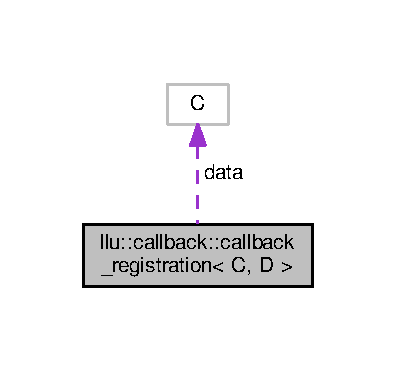
\includegraphics[width=190pt]{classllu_1_1callback_1_1callback__registration__coll__graph}
\end{center}
\end{figure}
\subsection*{Public Attributes}
\begin{DoxyCompactItemize}
\item 
void($\ast$ \hyperlink{classllu_1_1callback_1_1callback__registration_a470bbcee9d41e0070e9630461b88084d}{fnc} )(C, D)
\begin{DoxyCompactList}\small\item\em The pointer which will be caled if registered. \end{DoxyCompactList}\item 
C \hyperlink{classllu_1_1callback_1_1callback__registration_aecc9f23363c08b42144d70d928b4ec02}{data}
\begin{DoxyCompactList}\small\item\em The context of the callback, will be given to the fnc. \end{DoxyCompactList}\end{DoxyCompactItemize}


\subsection{Detailed Description}
\subsubsection*{template$<$typename C, typename D$>$class llu\+::callback\+::callback\+\_\+registration$<$ C, D $>$}

Calback registration, containing functon and. 

This class can be used for callback registration in an \hyperlink{classllu_1_1callback_1_1_callback}{Callback} class the C is the context of the function fnc, it will be the first parameter wen caled from \hyperlink{classllu_1_1callback_1_1_callback}{Callback} D is the sort of daten wich could be pased from a signal 

Definition at line 34 of file callback.\+hpp.



\subsection{Member Data Documentation}
\hypertarget{classllu_1_1callback_1_1callback__registration_aecc9f23363c08b42144d70d928b4ec02}{\index{llu\+::callback\+::callback\+\_\+registration@{llu\+::callback\+::callback\+\_\+registration}!data@{data}}
\index{data@{data}!llu\+::callback\+::callback\+\_\+registration@{llu\+::callback\+::callback\+\_\+registration}}
\subsubsection[{data}]{\setlength{\rightskip}{0pt plus 5cm}template$<$typename C, typename D$>$ C {\bf llu\+::callback\+::callback\+\_\+registration}$<$ C, D $>$\+::data}}\label{classllu_1_1callback_1_1callback__registration_aecc9f23363c08b42144d70d928b4ec02}


The context of the callback, will be given to the fnc. 

This will be given to the function fnc everytime it is caled from the \hyperlink{classllu_1_1callback_1_1_callback}{Callback} handler Class. it could be used to give the fnc a Object of some sort. \begin{DoxyNote}{Note}
will not be thread save 
\end{DoxyNote}


Definition at line 42 of file callback.\+hpp.

\hypertarget{classllu_1_1callback_1_1callback__registration_a470bbcee9d41e0070e9630461b88084d}{\index{llu\+::callback\+::callback\+\_\+registration@{llu\+::callback\+::callback\+\_\+registration}!fnc@{fnc}}
\index{fnc@{fnc}!llu\+::callback\+::callback\+\_\+registration@{llu\+::callback\+::callback\+\_\+registration}}
\subsubsection[{fnc}]{\setlength{\rightskip}{0pt plus 5cm}template$<$typename C, typename D$>$ void($\ast$ {\bf llu\+::callback\+::callback\+\_\+registration}$<$ C, D $>$\+::fnc)(C, D)}}\label{classllu_1_1callback_1_1callback__registration_a470bbcee9d41e0070e9630461b88084d}


The pointer which will be caled if registered. 

must acept an C at first place and data D at the second, twill be called form context in an own thread should not implement a hole bunch of functionality. 

Definition at line 36 of file callback.\+hpp.



The documentation for this class was generated from the following file\+:\begin{DoxyCompactItemize}
\item 
time\+Mux/\hyperlink{callback_8hpp}{callback.\+hpp}\end{DoxyCompactItemize}

\hypertarget{classllu_1_1network_1_1_connection}{\section{llu\+:\+:network\+:\+:Connection Class Reference}
\label{classllu_1_1network_1_1_connection}\index{llu\+::network\+::\+Connection@{llu\+::network\+::\+Connection}}
}


{\ttfamily \#include $<$network.\+hpp$>$}



Inheritance diagram for llu\+:\+:network\+:\+:Connection\+:
\nopagebreak
\begin{figure}[H]
\begin{center}
\leavevmode
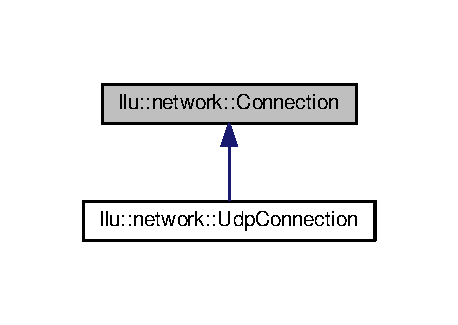
\includegraphics[width=220pt]{classllu_1_1network_1_1_connection__inherit__graph}
\end{center}
\end{figure}
\subsection*{Public Member Functions}
\begin{DoxyCompactItemize}
\item 
virtual \hyperlink{classllu_1_1network_1_1_connection_ad549cc793bf214a9097a62fa7fc01b33}{$\sim$\+Connection} ()
\item 
virtual \hyperlink{structllu_1_1network_1_1recived_message}{recived\+Message} $\ast$ \hyperlink{classllu_1_1network_1_1_connection_aae606f5aad246e892db5665cd7be1747}{recv\+Msg} ()=0
\begin{DoxyCompactList}\small\item\em recives a \hyperlink{structllu_1_1network_1_1recived_message}{recived\+Message} from the connection \end{DoxyCompactList}\item 
virtual void \hyperlink{classllu_1_1network_1_1_connection_ac20ca6d4d56b39fadde27b6af10000ae}{send\+Msg} (\hyperlink{structllu_1_1network_1_1send_message}{send\+Message} $\ast$m)=0
\begin{DoxyCompactList}\small\item\em sends the message m over the \hyperlink{classllu_1_1network_1_1_connection}{Connection} \end{DoxyCompactList}\item 
virtual bool \hyperlink{classllu_1_1network_1_1_connection_a05893a11a26ea97663637cf085e1b985}{alive} ()=0
\begin{DoxyCompactList}\small\item\em used to check if the connection is usable \end{DoxyCompactList}\item 
virtual void \hyperlink{classllu_1_1network_1_1_connection_a7e620755dde598fffc96d3ee6b3326a1}{kill} ()=0
\begin{DoxyCompactList}\small\item\em closes a connection \end{DoxyCompactList}\end{DoxyCompactItemize}


\subsection{Detailed Description}


Definition at line 153 of file network.\+hpp.



\subsection{Constructor \& Destructor Documentation}
\hypertarget{classllu_1_1network_1_1_connection_ad549cc793bf214a9097a62fa7fc01b33}{\index{llu\+::network\+::\+Connection@{llu\+::network\+::\+Connection}!````~Connection@{$\sim$\+Connection}}
\index{````~Connection@{$\sim$\+Connection}!llu\+::network\+::\+Connection@{llu\+::network\+::\+Connection}}
\subsubsection[{$\sim$\+Connection}]{\setlength{\rightskip}{0pt plus 5cm}virtual llu\+::network\+::\+Connection\+::$\sim$\+Connection (
\begin{DoxyParamCaption}
{}
\end{DoxyParamCaption}
)\hspace{0.3cm}{\ttfamily [inline]}, {\ttfamily [virtual]}}}\label{classllu_1_1network_1_1_connection_ad549cc793bf214a9097a62fa7fc01b33}


Definition at line 156 of file network.\+hpp.



\subsection{Member Function Documentation}
\hypertarget{classllu_1_1network_1_1_connection_a05893a11a26ea97663637cf085e1b985}{\index{llu\+::network\+::\+Connection@{llu\+::network\+::\+Connection}!alive@{alive}}
\index{alive@{alive}!llu\+::network\+::\+Connection@{llu\+::network\+::\+Connection}}
\subsubsection[{alive}]{\setlength{\rightskip}{0pt plus 5cm}virtual bool llu\+::network\+::\+Connection\+::alive (
\begin{DoxyParamCaption}
{}
\end{DoxyParamCaption}
)\hspace{0.3cm}{\ttfamily [pure virtual]}}}\label{classllu_1_1network_1_1_connection_a05893a11a26ea97663637cf085e1b985}


used to check if the connection is usable 

\begin{DoxyReturn}{Returns}
true if usable, otherwise false 
\end{DoxyReturn}


Implemented in \hyperlink{classllu_1_1network_1_1_udp_connection_add200cb20d4ece925b8752675d375828}{llu\+::network\+::\+Udp\+Connection}.

\hypertarget{classllu_1_1network_1_1_connection_a7e620755dde598fffc96d3ee6b3326a1}{\index{llu\+::network\+::\+Connection@{llu\+::network\+::\+Connection}!kill@{kill}}
\index{kill@{kill}!llu\+::network\+::\+Connection@{llu\+::network\+::\+Connection}}
\subsubsection[{kill}]{\setlength{\rightskip}{0pt plus 5cm}virtual void llu\+::network\+::\+Connection\+::kill (
\begin{DoxyParamCaption}
{}
\end{DoxyParamCaption}
)\hspace{0.3cm}{\ttfamily [pure virtual]}}}\label{classllu_1_1network_1_1_connection_a7e620755dde598fffc96d3ee6b3326a1}


closes a connection 



Implemented in \hyperlink{classllu_1_1network_1_1_udp_connection_a97a62c2ab3975d9716f965aacc2f28fc}{llu\+::network\+::\+Udp\+Connection}.

\hypertarget{classllu_1_1network_1_1_connection_aae606f5aad246e892db5665cd7be1747}{\index{llu\+::network\+::\+Connection@{llu\+::network\+::\+Connection}!recv\+Msg@{recv\+Msg}}
\index{recv\+Msg@{recv\+Msg}!llu\+::network\+::\+Connection@{llu\+::network\+::\+Connection}}
\subsubsection[{recv\+Msg}]{\setlength{\rightskip}{0pt plus 5cm}virtual {\bf recived\+Message}$\ast$ llu\+::network\+::\+Connection\+::recv\+Msg (
\begin{DoxyParamCaption}
{}
\end{DoxyParamCaption}
)\hspace{0.3cm}{\ttfamily [pure virtual]}}}\label{classllu_1_1network_1_1_connection_aae606f5aad246e892db5665cd7be1747}


recives a \hyperlink{structllu_1_1network_1_1recived_message}{recived\+Message} from the connection 

Blocks untill data is avaliable \begin{DoxyReturn}{Returns}
the \hyperlink{structllu_1_1network_1_1recived_message}{recived\+Message} rescived the responsebilety for the result belonges to the caller 
\end{DoxyReturn}


Implemented in \hyperlink{classllu_1_1network_1_1_udp_connection_abbd9d3906a283f5506a69a8922fa76c6}{llu\+::network\+::\+Udp\+Connection}.

\hypertarget{classllu_1_1network_1_1_connection_ac20ca6d4d56b39fadde27b6af10000ae}{\index{llu\+::network\+::\+Connection@{llu\+::network\+::\+Connection}!send\+Msg@{send\+Msg}}
\index{send\+Msg@{send\+Msg}!llu\+::network\+::\+Connection@{llu\+::network\+::\+Connection}}
\subsubsection[{send\+Msg}]{\setlength{\rightskip}{0pt plus 5cm}virtual void llu\+::network\+::\+Connection\+::send\+Msg (
\begin{DoxyParamCaption}
\item[{{\bf send\+Message} $\ast$}]{m}
\end{DoxyParamCaption}
)\hspace{0.3cm}{\ttfamily [pure virtual]}}}\label{classllu_1_1network_1_1_connection_ac20ca6d4d56b39fadde27b6af10000ae}


sends the message m over the \hyperlink{classllu_1_1network_1_1_connection}{Connection} 

this methode is not blocking m will be deletet using destory\+Send\+Message 

Implemented in \hyperlink{classllu_1_1network_1_1_udp_connection_a044432ee61191ecabd295fe4ea6cddf1}{llu\+::network\+::\+Udp\+Connection}.



The documentation for this class was generated from the following file\+:\begin{DoxyCompactItemize}
\item 
time\+Mux/\hyperlink{network_8hpp}{network.\+hpp}\end{DoxyCompactItemize}

\hypertarget{classllu_1_1datastructs_1_1_linked_list}{\section{llu\+:\+:datastructs\+:\+:Linked\+List$<$ E $>$ Class Template Reference}
\label{classllu_1_1datastructs_1_1_linked_list}\index{llu\+::datastructs\+::\+Linked\+List$<$ E $>$@{llu\+::datastructs\+::\+Linked\+List$<$ E $>$}}
}


very spartanic implementation of a generik thread save Linked list  




{\ttfamily \#include $<$linked\+List.\+hpp$>$}

\subsection*{Public Member Functions}
\begin{DoxyCompactItemize}
\item 
\hyperlink{classllu_1_1datastructs_1_1_linked_list_ae12ddd9d50e228bc8602e902c2e4909e}{Linked\+List} ()
\begin{DoxyCompactList}\small\item\em creates an empty linked list \end{DoxyCompactList}\item 
\hyperlink{classllu_1_1datastructs_1_1_linked_list_a9d51cbffdc243ae0831d7c91a7da528a}{$\sim$\+Linked\+List} ()
\begin{DoxyCompactList}\small\item\em deletes the linekd list and clears memory \end{DoxyCompactList}\item 
void \hyperlink{classllu_1_1datastructs_1_1_linked_list_afb594d9c6ee789ba60070365e8953a29}{append} (E \hyperlink{timux_8hpp_ad9c7575237a3a2780e8e6d16e1334982}{data})
\begin{DoxyCompactList}\small\item\em appends data to the end of the list \end{DoxyCompactList}\item 
bool \hyperlink{classllu_1_1datastructs_1_1_linked_list_a89e2f65a016e358dc174921d496e34ce}{contains} (bool($\ast$comparer)(E, E), E elem)
\begin{DoxyCompactList}\small\item\em checks if the given element elem is contaned in the list \end{DoxyCompactList}\end{DoxyCompactItemize}
\subsection*{Public Attributes}
\begin{DoxyCompactItemize}
\item 
\hyperlink{structllu_1_1datastructs_1_1list_entrie}{list\+Entrie}$<$ E $>$ \hyperlink{classllu_1_1datastructs_1_1_linked_list_a2d5511009cd4b6579b8978af4f23c148}{start}
\begin{DoxyCompactList}\small\item\em the first element of the linekd list \end{DoxyCompactList}\item 
std\+::mutex \hyperlink{classllu_1_1datastructs_1_1_linked_list_abe1e82a0eab42b3ad2f0903a17c8003d}{lock}
\begin{DoxyCompactList}\small\item\em Lock for accessing the linekd list threadsave. \end{DoxyCompactList}\end{DoxyCompactItemize}


\subsection{Detailed Description}
\subsubsection*{template$<$typename E$>$class llu\+::datastructs\+::\+Linked\+List$<$ E $>$}

very spartanic implementation of a generik thread save Linked list 

The type E defines the type of elements to put in the list To get the data from the list it is nessasary to direkly use the \hyperlink{structllu_1_1datastructs_1_1list_entrie}{list\+Entrie} start The list is single linked 

Definition at line 34 of file linked\+List.\+hpp.



\subsection{Constructor \& Destructor Documentation}
\hypertarget{classllu_1_1datastructs_1_1_linked_list_ae12ddd9d50e228bc8602e902c2e4909e}{\index{llu\+::datastructs\+::\+Linked\+List@{llu\+::datastructs\+::\+Linked\+List}!Linked\+List@{Linked\+List}}
\index{Linked\+List@{Linked\+List}!llu\+::datastructs\+::\+Linked\+List@{llu\+::datastructs\+::\+Linked\+List}}
\subsubsection[{Linked\+List}]{\setlength{\rightskip}{0pt plus 5cm}template$<$typename E$>$ {\bf llu\+::datastructs\+::\+Linked\+List}$<$ E $>$\+::{\bf Linked\+List} (
\begin{DoxyParamCaption}
{}
\end{DoxyParamCaption}
)\hspace{0.3cm}{\ttfamily [inline]}}}\label{classllu_1_1datastructs_1_1_linked_list_ae12ddd9d50e228bc8602e902c2e4909e}


creates an empty linked list 



Definition at line 40 of file linked\+List.\+hpp.

\hypertarget{classllu_1_1datastructs_1_1_linked_list_a9d51cbffdc243ae0831d7c91a7da528a}{\index{llu\+::datastructs\+::\+Linked\+List@{llu\+::datastructs\+::\+Linked\+List}!````~Linked\+List@{$\sim$\+Linked\+List}}
\index{````~Linked\+List@{$\sim$\+Linked\+List}!llu\+::datastructs\+::\+Linked\+List@{llu\+::datastructs\+::\+Linked\+List}}
\subsubsection[{$\sim$\+Linked\+List}]{\setlength{\rightskip}{0pt plus 5cm}template$<$typename E$>$ {\bf llu\+::datastructs\+::\+Linked\+List}$<$ E $>$\+::$\sim${\bf Linked\+List} (
\begin{DoxyParamCaption}
{}
\end{DoxyParamCaption}
)\hspace{0.3cm}{\ttfamily [inline]}}}\label{classllu_1_1datastructs_1_1_linked_list_a9d51cbffdc243ae0831d7c91a7da528a}


deletes the linekd list and clears memory 

\begin{DoxyNote}{Note}
the data which is in the list, will not be cleared 
\end{DoxyNote}


Definition at line 46 of file linked\+List.\+hpp.



\subsection{Member Function Documentation}
\hypertarget{classllu_1_1datastructs_1_1_linked_list_afb594d9c6ee789ba60070365e8953a29}{\index{llu\+::datastructs\+::\+Linked\+List@{llu\+::datastructs\+::\+Linked\+List}!append@{append}}
\index{append@{append}!llu\+::datastructs\+::\+Linked\+List@{llu\+::datastructs\+::\+Linked\+List}}
\subsubsection[{append}]{\setlength{\rightskip}{0pt plus 5cm}template$<$typename E$>$ void {\bf llu\+::datastructs\+::\+Linked\+List}$<$ E $>$\+::append (
\begin{DoxyParamCaption}
\item[{E}]{data}
\end{DoxyParamCaption}
)\hspace{0.3cm}{\ttfamily [inline]}}}\label{classllu_1_1datastructs_1_1_linked_list_afb594d9c6ee789ba60070365e8953a29}


appends data to the end of the list 


\begin{DoxyParams}{Parameters}
{\em data} & the data to append to the list \\
\hline
\end{DoxyParams}


Definition at line 75 of file linked\+List.\+hpp.

\hypertarget{classllu_1_1datastructs_1_1_linked_list_a89e2f65a016e358dc174921d496e34ce}{\index{llu\+::datastructs\+::\+Linked\+List@{llu\+::datastructs\+::\+Linked\+List}!contains@{contains}}
\index{contains@{contains}!llu\+::datastructs\+::\+Linked\+List@{llu\+::datastructs\+::\+Linked\+List}}
\subsubsection[{contains}]{\setlength{\rightskip}{0pt plus 5cm}template$<$typename E$>$ bool {\bf llu\+::datastructs\+::\+Linked\+List}$<$ E $>$\+::contains (
\begin{DoxyParamCaption}
\item[{bool($\ast$)(E, E)}]{comparer, }
\item[{E}]{elem}
\end{DoxyParamCaption}
)\hspace{0.3cm}{\ttfamily [inline]}}}\label{classllu_1_1datastructs_1_1_linked_list_a89e2f65a016e358dc174921d496e34ce}


checks if the given element elem is contaned in the list 


\begin{DoxyParams}{Parameters}
{\em comparer} & is used to check if two elements of type E are equal \\
\hline
{\em elem} & the element to check for \\
\hline
\end{DoxyParams}
\begin{DoxyReturn}{Returns}
true if elem is in the list otherwise false 
\end{DoxyReturn}


Definition at line 99 of file linked\+List.\+hpp.



\subsection{Member Data Documentation}
\hypertarget{classllu_1_1datastructs_1_1_linked_list_abe1e82a0eab42b3ad2f0903a17c8003d}{\index{llu\+::datastructs\+::\+Linked\+List@{llu\+::datastructs\+::\+Linked\+List}!lock@{lock}}
\index{lock@{lock}!llu\+::datastructs\+::\+Linked\+List@{llu\+::datastructs\+::\+Linked\+List}}
\subsubsection[{lock}]{\setlength{\rightskip}{0pt plus 5cm}template$<$typename E$>$ std\+::mutex {\bf llu\+::datastructs\+::\+Linked\+List}$<$ E $>$\+::lock}}\label{classllu_1_1datastructs_1_1_linked_list_abe1e82a0eab42b3ad2f0903a17c8003d}


Lock for accessing the linekd list threadsave. 

this must be used, wenn iterating manualy over the list 

Definition at line 69 of file linked\+List.\+hpp.

\hypertarget{classllu_1_1datastructs_1_1_linked_list_a2d5511009cd4b6579b8978af4f23c148}{\index{llu\+::datastructs\+::\+Linked\+List@{llu\+::datastructs\+::\+Linked\+List}!start@{start}}
\index{start@{start}!llu\+::datastructs\+::\+Linked\+List@{llu\+::datastructs\+::\+Linked\+List}}
\subsubsection[{start}]{\setlength{\rightskip}{0pt plus 5cm}template$<$typename E$>$ {\bf list\+Entrie}$<$E$>$ {\bf llu\+::datastructs\+::\+Linked\+List}$<$ E $>$\+::start}}\label{classllu_1_1datastructs_1_1_linked_list_a2d5511009cd4b6579b8978af4f23c148}


the first element of the linekd list 

it does not contain any user data, and must be used to start the interating of the list. 

Definition at line 62 of file linked\+List.\+hpp.



The documentation for this class was generated from the following file\+:\begin{DoxyCompactItemize}
\item 
time\+Mux/\hyperlink{linked_list_8hpp}{linked\+List.\+hpp}\end{DoxyCompactItemize}

\hypertarget{classllu_1_1datastructs_1_1_linked_list_array}{\section{llu\+:\+:datastructs\+:\+:Linked\+List\+Array$<$ E $>$ Class Template Reference}
\label{classllu_1_1datastructs_1_1_linked_list_array}\index{llu\+::datastructs\+::\+Linked\+List\+Array$<$ E $>$@{llu\+::datastructs\+::\+Linked\+List\+Array$<$ E $>$}}
}


Implementation of a simple generik thread save Array.  




{\ttfamily \#include $<$linked\+Array.\+hpp$>$}

\subsection*{Public Member Functions}
\begin{DoxyCompactItemize}
\item 
\hyperlink{classllu_1_1datastructs_1_1_linked_list_array_abc6ac1822c04f74d5df08c500fb404c1}{Linked\+List\+Array} ()
\begin{DoxyCompactList}\small\item\em creates an empty \hyperlink{classllu_1_1datastructs_1_1_linked_list_array}{Linked\+List\+Array} with the default value ((E)N\+U\+L\+L) \end{DoxyCompactList}\item 
\hyperlink{classllu_1_1datastructs_1_1_linked_list_array_aed92b975cd23466ae97c8348a6caaf10}{Linked\+List\+Array} (E default\+Value)
\begin{DoxyCompactList}\small\item\em creates an empty \hyperlink{classllu_1_1datastructs_1_1_linked_list_array}{Linked\+List\+Array} with the spezified default value \end{DoxyCompactList}\item 
\hyperlink{classllu_1_1datastructs_1_1_linked_list_array_a4afa917caa5b398d66cf0853f7f258b9}{$\sim$\+Linked\+List\+Array} ()
\begin{DoxyCompactList}\small\item\em deletes this objekt, an clears memory \end{DoxyCompactList}\item 
int \hyperlink{classllu_1_1datastructs_1_1_linked_list_array_ac588bbfb35a0903ad5c782d11ec0f334}{put} (unsigned int index, E \hyperlink{timux_8hpp_ad9c7575237a3a2780e8e6d16e1334982}{data})
\begin{DoxyCompactList}\small\item\em Puts the element data at position index. \end{DoxyCompactList}\item 
E \hyperlink{classllu_1_1datastructs_1_1_linked_list_array_a9ed83912b4cb5d14512d087ebbb2f8e9}{get} (unsigned int index)
\begin{DoxyCompactList}\small\item\em returns an element from index \end{DoxyCompactList}\end{DoxyCompactItemize}
\subsection*{Public Attributes}
\begin{DoxyCompactItemize}
\item 
std\+::mutex \hyperlink{classllu_1_1datastructs_1_1_linked_list_array_a7c9cdd61e7665e7f97447e25ca64451e}{lock}
\begin{DoxyCompactList}\small\item\em lock for the Array. \end{DoxyCompactList}\item 
\hyperlink{structllu_1_1datastructs_1_1list_array_entrie}{list\+Array\+Entrie}$<$ E $>$ \hyperlink{classllu_1_1datastructs_1_1_linked_list_array_ac6470a016e4ca99b16ab57db1b6f1f26}{start}
\begin{DoxyCompactList}\small\item\em the first element of the list\+Array \end{DoxyCompactList}\end{DoxyCompactItemize}


\subsection{Detailed Description}
\subsubsection*{template$<$typename E$>$class llu\+::datastructs\+::\+Linked\+List\+Array$<$ E $>$}

Implementation of a simple generik thread save Array. 

internely this class is implemented as a linked List. therefor the differences in the indizes can be enormus, without much memory consumtion, \begin{DoxyNote}{Note}
compared to a regular array this is very slow, should not be used if a normal array would fit the task 
\end{DoxyNote}


Definition at line 37 of file linked\+Array.\+hpp.



\subsection{Constructor \& Destructor Documentation}
\hypertarget{classllu_1_1datastructs_1_1_linked_list_array_abc6ac1822c04f74d5df08c500fb404c1}{\index{llu\+::datastructs\+::\+Linked\+List\+Array@{llu\+::datastructs\+::\+Linked\+List\+Array}!Linked\+List\+Array@{Linked\+List\+Array}}
\index{Linked\+List\+Array@{Linked\+List\+Array}!llu\+::datastructs\+::\+Linked\+List\+Array@{llu\+::datastructs\+::\+Linked\+List\+Array}}
\subsubsection[{Linked\+List\+Array}]{\setlength{\rightskip}{0pt plus 5cm}template$<$typename E$>$ {\bf llu\+::datastructs\+::\+Linked\+List\+Array}$<$ E $>$\+::{\bf Linked\+List\+Array} (
\begin{DoxyParamCaption}
{}
\end{DoxyParamCaption}
)\hspace{0.3cm}{\ttfamily [inline]}}}\label{classllu_1_1datastructs_1_1_linked_list_array_abc6ac1822c04f74d5df08c500fb404c1}


creates an empty \hyperlink{classllu_1_1datastructs_1_1_linked_list_array}{Linked\+List\+Array} with the default value ((E)N\+U\+L\+L) 



Definition at line 42 of file linked\+Array.\+hpp.

\hypertarget{classllu_1_1datastructs_1_1_linked_list_array_aed92b975cd23466ae97c8348a6caaf10}{\index{llu\+::datastructs\+::\+Linked\+List\+Array@{llu\+::datastructs\+::\+Linked\+List\+Array}!Linked\+List\+Array@{Linked\+List\+Array}}
\index{Linked\+List\+Array@{Linked\+List\+Array}!llu\+::datastructs\+::\+Linked\+List\+Array@{llu\+::datastructs\+::\+Linked\+List\+Array}}
\subsubsection[{Linked\+List\+Array}]{\setlength{\rightskip}{0pt plus 5cm}template$<$typename E$>$ {\bf llu\+::datastructs\+::\+Linked\+List\+Array}$<$ E $>$\+::{\bf Linked\+List\+Array} (
\begin{DoxyParamCaption}
\item[{E}]{default\+Value}
\end{DoxyParamCaption}
)\hspace{0.3cm}{\ttfamily [inline]}}}\label{classllu_1_1datastructs_1_1_linked_list_array_aed92b975cd23466ae97c8348a6caaf10}


creates an empty \hyperlink{classllu_1_1datastructs_1_1_linked_list_array}{Linked\+List\+Array} with the spezified default value 


\begin{DoxyParams}{Parameters}
{\em default\+Value} & The default value for en empty cell \\
\hline
\end{DoxyParams}


Definition at line 50 of file linked\+Array.\+hpp.

\hypertarget{classllu_1_1datastructs_1_1_linked_list_array_a4afa917caa5b398d66cf0853f7f258b9}{\index{llu\+::datastructs\+::\+Linked\+List\+Array@{llu\+::datastructs\+::\+Linked\+List\+Array}!````~Linked\+List\+Array@{$\sim$\+Linked\+List\+Array}}
\index{````~Linked\+List\+Array@{$\sim$\+Linked\+List\+Array}!llu\+::datastructs\+::\+Linked\+List\+Array@{llu\+::datastructs\+::\+Linked\+List\+Array}}
\subsubsection[{$\sim$\+Linked\+List\+Array}]{\setlength{\rightskip}{0pt plus 5cm}template$<$typename E$>$ {\bf llu\+::datastructs\+::\+Linked\+List\+Array}$<$ E $>$\+::$\sim${\bf Linked\+List\+Array} (
\begin{DoxyParamCaption}
{}
\end{DoxyParamCaption}
)\hspace{0.3cm}{\ttfamily [inline]}}}\label{classllu_1_1datastructs_1_1_linked_list_array_a4afa917caa5b398d66cf0853f7f258b9}


deletes this objekt, an clears memory 

\begin{DoxyNote}{Note}
the stored data is still preserved, and must be cleared elsewere 
\end{DoxyNote}


Definition at line 58 of file linked\+Array.\+hpp.



\subsection{Member Function Documentation}
\hypertarget{classllu_1_1datastructs_1_1_linked_list_array_a9ed83912b4cb5d14512d087ebbb2f8e9}{\index{llu\+::datastructs\+::\+Linked\+List\+Array@{llu\+::datastructs\+::\+Linked\+List\+Array}!get@{get}}
\index{get@{get}!llu\+::datastructs\+::\+Linked\+List\+Array@{llu\+::datastructs\+::\+Linked\+List\+Array}}
\subsubsection[{get}]{\setlength{\rightskip}{0pt plus 5cm}template$<$typename E$>$ E {\bf llu\+::datastructs\+::\+Linked\+List\+Array}$<$ E $>$\+::get (
\begin{DoxyParamCaption}
\item[{unsigned int}]{index}
\end{DoxyParamCaption}
)\hspace{0.3cm}{\ttfamily [inline]}}}\label{classllu_1_1datastructs_1_1_linked_list_array_a9ed83912b4cb5d14512d087ebbb2f8e9}


returns an element from index 


\begin{DoxyParams}{Parameters}
{\em index} & the index to get the element from \\
\hline
\end{DoxyParams}
\begin{DoxyReturn}{Returns}
the element at index if there is no element at index, it will return the default value 
\end{DoxyReturn}


Definition at line 127 of file linked\+Array.\+hpp.

\hypertarget{classllu_1_1datastructs_1_1_linked_list_array_ac588bbfb35a0903ad5c782d11ec0f334}{\index{llu\+::datastructs\+::\+Linked\+List\+Array@{llu\+::datastructs\+::\+Linked\+List\+Array}!put@{put}}
\index{put@{put}!llu\+::datastructs\+::\+Linked\+List\+Array@{llu\+::datastructs\+::\+Linked\+List\+Array}}
\subsubsection[{put}]{\setlength{\rightskip}{0pt plus 5cm}template$<$typename E$>$ int {\bf llu\+::datastructs\+::\+Linked\+List\+Array}$<$ E $>$\+::put (
\begin{DoxyParamCaption}
\item[{unsigned int}]{index, }
\item[{E}]{data}
\end{DoxyParamCaption}
)\hspace{0.3cm}{\ttfamily [inline]}}}\label{classllu_1_1datastructs_1_1_linked_list_array_ac588bbfb35a0903ad5c782d11ec0f334}


Puts the element data at position index. 

can be used to put an element at a spezific index, if the index was allready taken nothing would happen 
\begin{DoxyParams}{Parameters}
{\em index} & the inex in the array \\
\hline
{\em data} & of type E \\
\hline
\end{DoxyParams}
\begin{DoxyReturn}{Returns}
0 if nothing was done otherwise 1 
\end{DoxyReturn}


Definition at line 93 of file linked\+Array.\+hpp.



\subsection{Member Data Documentation}
\hypertarget{classllu_1_1datastructs_1_1_linked_list_array_a7c9cdd61e7665e7f97447e25ca64451e}{\index{llu\+::datastructs\+::\+Linked\+List\+Array@{llu\+::datastructs\+::\+Linked\+List\+Array}!lock@{lock}}
\index{lock@{lock}!llu\+::datastructs\+::\+Linked\+List\+Array@{llu\+::datastructs\+::\+Linked\+List\+Array}}
\subsubsection[{lock}]{\setlength{\rightskip}{0pt plus 5cm}template$<$typename E$>$ std\+::mutex {\bf llu\+::datastructs\+::\+Linked\+List\+Array}$<$ E $>$\+::lock}}\label{classllu_1_1datastructs_1_1_linked_list_array_a7c9cdd61e7665e7f97447e25ca64451e}


lock for the Array. 

\begin{DoxyNote}{Note}
should be used, if accessing the Raw Linked List from outside 
\end{DoxyNote}


Definition at line 75 of file linked\+Array.\+hpp.

\hypertarget{classllu_1_1datastructs_1_1_linked_list_array_ac6470a016e4ca99b16ab57db1b6f1f26}{\index{llu\+::datastructs\+::\+Linked\+List\+Array@{llu\+::datastructs\+::\+Linked\+List\+Array}!start@{start}}
\index{start@{start}!llu\+::datastructs\+::\+Linked\+List\+Array@{llu\+::datastructs\+::\+Linked\+List\+Array}}
\subsubsection[{start}]{\setlength{\rightskip}{0pt plus 5cm}template$<$typename E$>$ {\bf list\+Array\+Entrie}$<$E$>$ {\bf llu\+::datastructs\+::\+Linked\+List\+Array}$<$ E $>$\+::start}}\label{classllu_1_1datastructs_1_1_linked_list_array_ac6470a016e4ca99b16ab57db1b6f1f26}


the first element of the list\+Array 

no actual user data is stored here, it is an empty element. can be used to acces the Raw linked list 

Definition at line 83 of file linked\+Array.\+hpp.



The documentation for this class was generated from the following file\+:\begin{DoxyCompactItemize}
\item 
time\+Mux/\hyperlink{linked_array_8hpp}{linked\+Array.\+hpp}\end{DoxyCompactItemize}

\hypertarget{structllu_1_1datastructs_1_1list_array_entrie}{\section{llu\+:\+:datastructs\+:\+:list\+Array\+Entrie$<$ E $>$ Struct Template Reference}
\label{structllu_1_1datastructs_1_1list_array_entrie}\index{llu\+::datastructs\+::list\+Array\+Entrie$<$ E $>$@{llu\+::datastructs\+::list\+Array\+Entrie$<$ E $>$}}
}


An entry of an list\+Array of type E.  




{\ttfamily \#include $<$linked\+Array.\+hpp$>$}



Collaboration diagram for llu\+:\+:datastructs\+:\+:list\+Array\+Entrie$<$ E $>$\+:
\nopagebreak
\begin{figure}[H]
\begin{center}
\leavevmode
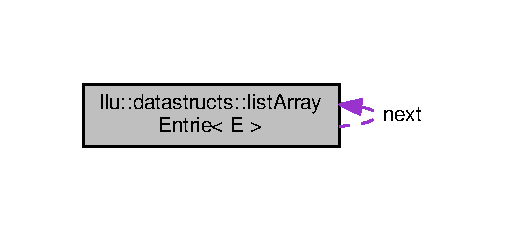
\includegraphics[width=243pt]{structllu_1_1datastructs_1_1list_array_entrie__coll__graph}
\end{center}
\end{figure}
\subsection*{Public Attributes}
\begin{DoxyCompactItemize}
\item 
struct \hyperlink{structllu_1_1datastructs_1_1list_array_entrie}{list\+Array\+Entrie} $\ast$ \hyperlink{structllu_1_1datastructs_1_1list_array_entrie_a110bf134b27bdfaa3ca518b40042591e}{next}
\begin{DoxyCompactList}\small\item\em a pointer to the next element in the list, or Null if there ist none \end{DoxyCompactList}\item 
unsigned int \hyperlink{structllu_1_1datastructs_1_1list_array_entrie_aed7349160256aefaca0cf5b4caba9de7}{index}
\begin{DoxyCompactList}\small\item\em the ined of the entry in the compleet artray \end{DoxyCompactList}\item 
E \hyperlink{structllu_1_1datastructs_1_1list_array_entrie_a495283bde8e6a508d470e19d39328b39}{data}
\begin{DoxyCompactList}\small\item\em the data stored in the cell can be everything of type E \end{DoxyCompactList}\end{DoxyCompactItemize}


\subsection{Detailed Description}
\subsubsection*{template$<$typename E$>$struct llu\+::datastructs\+::list\+Array\+Entrie$<$ E $>$}

An entry of an list\+Array of type E. 

Can be used to iterate over an compleate list\+Array, or to manipolate the data in normaly not supported ways, the list array should be locked during this 

Definition at line 22 of file linked\+Array.\+hpp.



\subsection{Member Data Documentation}
\hypertarget{structllu_1_1datastructs_1_1list_array_entrie_a495283bde8e6a508d470e19d39328b39}{\index{llu\+::datastructs\+::list\+Array\+Entrie@{llu\+::datastructs\+::list\+Array\+Entrie}!data@{data}}
\index{data@{data}!llu\+::datastructs\+::list\+Array\+Entrie@{llu\+::datastructs\+::list\+Array\+Entrie}}
\subsubsection[{data}]{\setlength{\rightskip}{0pt plus 5cm}template$<$typename E$>$ E {\bf llu\+::datastructs\+::list\+Array\+Entrie}$<$ E $>$\+::data}}\label{structllu_1_1datastructs_1_1list_array_entrie_a495283bde8e6a508d470e19d39328b39}


the data stored in the cell can be everything of type E 



Definition at line 27 of file linked\+Array.\+hpp.

\hypertarget{structllu_1_1datastructs_1_1list_array_entrie_aed7349160256aefaca0cf5b4caba9de7}{\index{llu\+::datastructs\+::list\+Array\+Entrie@{llu\+::datastructs\+::list\+Array\+Entrie}!index@{index}}
\index{index@{index}!llu\+::datastructs\+::list\+Array\+Entrie@{llu\+::datastructs\+::list\+Array\+Entrie}}
\subsubsection[{index}]{\setlength{\rightskip}{0pt plus 5cm}template$<$typename E$>$ unsigned int {\bf llu\+::datastructs\+::list\+Array\+Entrie}$<$ E $>$\+::index}}\label{structllu_1_1datastructs_1_1list_array_entrie_aed7349160256aefaca0cf5b4caba9de7}


the ined of the entry in the compleet artray 

\begin{DoxyNote}{Note}
it is importante that the list is sorted 
\end{DoxyNote}


Definition at line 24 of file linked\+Array.\+hpp.

\hypertarget{structllu_1_1datastructs_1_1list_array_entrie_a110bf134b27bdfaa3ca518b40042591e}{\index{llu\+::datastructs\+::list\+Array\+Entrie@{llu\+::datastructs\+::list\+Array\+Entrie}!next@{next}}
\index{next@{next}!llu\+::datastructs\+::list\+Array\+Entrie@{llu\+::datastructs\+::list\+Array\+Entrie}}
\subsubsection[{next}]{\setlength{\rightskip}{0pt plus 5cm}template$<$typename E$>$ struct {\bf list\+Array\+Entrie}$\ast$ {\bf llu\+::datastructs\+::list\+Array\+Entrie}$<$ E $>$\+::next}}\label{structllu_1_1datastructs_1_1list_array_entrie_a110bf134b27bdfaa3ca518b40042591e}


a pointer to the next element in the list, or Null if there ist none 



Definition at line 23 of file linked\+Array.\+hpp.



The documentation for this struct was generated from the following file\+:\begin{DoxyCompactItemize}
\item 
time\+Mux/\hyperlink{linked_array_8hpp}{linked\+Array.\+hpp}\end{DoxyCompactItemize}

\hypertarget{structllu_1_1datastructs_1_1list_entrie}{\section{llu\+:\+:datastructs\+:\+:list\+Entrie$<$ E $>$ Struct Template Reference}
\label{structllu_1_1datastructs_1_1list_entrie}\index{llu\+::datastructs\+::list\+Entrie$<$ E $>$@{llu\+::datastructs\+::list\+Entrie$<$ E $>$}}
}


an list entry for a linked list of type E  




{\ttfamily \#include $<$linked\+List.\+hpp$>$}

\subsection*{Public Attributes}
\begin{DoxyCompactItemize}
\item 
struct \hyperlink{structllu_1_1datastructs_1_1list_entrie}{list\+Entrie}$<$ E $>$ $\ast$ \hyperlink{structllu_1_1datastructs_1_1list_entrie_a3a0c3cef3ce8b0b9beaa1c6360fb6346}{next}
\begin{DoxyCompactList}\small\item\em Pointer to the next element of the linked list or null. \end{DoxyCompactList}\item 
E \hyperlink{structllu_1_1datastructs_1_1list_entrie_ae45377a6f71b68a0bd56844aedc52fb7}{data}
\begin{DoxyCompactList}\small\item\em The data of the element in the list. \end{DoxyCompactList}\end{DoxyCompactItemize}


\subsection{Detailed Description}
\subsubsection*{template$<$typename E$>$struct llu\+::datastructs\+::list\+Entrie$<$ E $>$}

an list entry for a linked list of type E 

Can be used to iterate over an compleate list\+Array, or to manipolate the data in normaly not supported ways, the list should be locked during this 

Definition at line 21 of file linked\+List.\+hpp.



\subsection{Member Data Documentation}
\hypertarget{structllu_1_1datastructs_1_1list_entrie_ae45377a6f71b68a0bd56844aedc52fb7}{\index{llu\+::datastructs\+::list\+Entrie@{llu\+::datastructs\+::list\+Entrie}!data@{data}}
\index{data@{data}!llu\+::datastructs\+::list\+Entrie@{llu\+::datastructs\+::list\+Entrie}}
\subsubsection[{data}]{\setlength{\rightskip}{0pt plus 5cm}template$<$typename E$>$ E {\bf llu\+::datastructs\+::list\+Entrie}$<$ E $>$\+::data}}\label{structllu_1_1datastructs_1_1list_entrie_ae45377a6f71b68a0bd56844aedc52fb7}


The data of the element in the list. 



Definition at line 23 of file linked\+List.\+hpp.

\hypertarget{structllu_1_1datastructs_1_1list_entrie_a3a0c3cef3ce8b0b9beaa1c6360fb6346}{\index{llu\+::datastructs\+::list\+Entrie@{llu\+::datastructs\+::list\+Entrie}!next@{next}}
\index{next@{next}!llu\+::datastructs\+::list\+Entrie@{llu\+::datastructs\+::list\+Entrie}}
\subsubsection[{next}]{\setlength{\rightskip}{0pt plus 5cm}template$<$typename E$>$ struct {\bf list\+Entrie}$<$ E $>$$\ast$ {\bf llu\+::datastructs\+::list\+Entrie}$<$ E $>$\+::next}}\label{structllu_1_1datastructs_1_1list_entrie_a3a0c3cef3ce8b0b9beaa1c6360fb6346}


Pointer to the next element of the linked list or null. 



Definition at line 22 of file linked\+List.\+hpp.



The documentation for this struct was generated from the following file\+:\begin{DoxyCompactItemize}
\item 
time\+Mux/\hyperlink{linked_list_8hpp}{linked\+List.\+hpp}\end{DoxyCompactItemize}

\hypertarget{classllu_1_1network_1_1_managed_connection}{\section{llu\+:\+:network\+:\+:Managed\+Connection Class Reference}
\label{classllu_1_1network_1_1_managed_connection}\index{llu\+::network\+::\+Managed\+Connection@{llu\+::network\+::\+Managed\+Connection}}
}


a Managed form of a \hyperlink{classllu_1_1network_1_1_connection}{Connection} implements callbacks on massage recive internayls uses a callback handler  




{\ttfamily \#include $<$network.\+hpp$>$}

\subsection*{Public Member Functions}
\begin{DoxyCompactItemize}
\item 
\hyperlink{classllu_1_1network_1_1_managed_connection_a799a62f147762b2c4992ce91f06ff451}{Managed\+Connection} (\hyperlink{classllu_1_1network_1_1_connection}{Connection} $\ast$con)
\begin{DoxyCompactList}\small\item\em wrapes a classic connection to make it managed \end{DoxyCompactList}\item 
\hyperlink{classllu_1_1network_1_1_managed_connection_ab2740d022d8af2679b76e3b7c097909c}{$\sim$\+Managed\+Connection} ()
\begin{DoxyCompactList}\small\item\em cleans up some stuff, also cloese the connection \end{DoxyCompactList}\item 
void \hyperlink{classllu_1_1network_1_1_managed_connection_a464e40505c93ce769dacf381a6e0e503}{send\+Msg} (\hyperlink{structllu_1_1network_1_1send_message}{send\+Message} $\ast$m)
\begin{DoxyCompactList}\small\item\em puts a massage in the out queue \end{DoxyCompactList}\item 
void \hyperlink{classllu_1_1network_1_1_managed_connection_a5bce6d60a66c9dc660b3cd20479830c9}{add\+Classifier} (\hyperlink{namespacellu_1_1network_ac629c1180a0bee8ddef541f73cb3e5f9}{recived\+Message\+Classifier} c)
\begin{DoxyCompactList}\small\item\em adds a massage clasifier for callbacks \end{DoxyCompactList}\item 
void \hyperlink{classllu_1_1network_1_1_managed_connection_a1348765635cc1e53340dc94c5879a4c6}{add\+Callback} (\hyperlink{namespacellu_1_1callback_a082ed24306809c4d250bd5ddfbae177f}{signal} s, \hyperlink{namespacellu_1_1network_a999d34263abe84a87d12271383c606b9}{netwok\+Msg\+Callback} $\ast$calback)
\begin{DoxyCompactList}\small\item\em adds a message recived callback \end{DoxyCompactList}\item 
void \hyperlink{classllu_1_1network_1_1_managed_connection_a04c4198e03082243885c058d7e703e8e}{kill} ()
\begin{DoxyCompactList}\small\item\em closes the mennaged and underlying unmanaged connection \end{DoxyCompactList}\item 
bool \hyperlink{classllu_1_1network_1_1_managed_connection_a21eb51f8f91b3103a71708c4b190784a}{alive} ()
\begin{DoxyCompactList}\small\item\em used to check if the connection is alvice \end{DoxyCompactList}\item 
\hyperlink{classllu_1_1network_1_1_connection}{Connection} $\ast$ \hyperlink{classllu_1_1network_1_1_managed_connection_a6b75597f4a9ed3be7202f5118383eba5}{raw} ()
\begin{DoxyCompactList}\small\item\em can be used to acces the underlaying connection \end{DoxyCompactList}\item 
void \hyperlink{classllu_1_1network_1_1_managed_connection_a2c5a8dca6f2cae9b3ae8f928a1c940ed}{lock\+Write} ()
\begin{DoxyCompactList}\small\item\em locks the connection for writing \end{DoxyCompactList}\item 
void \hyperlink{classllu_1_1network_1_1_managed_connection_a47c8c8c501e5794f2ab0ccd9faa16c2e}{unlock\+Write} ()
\begin{DoxyCompactList}\small\item\em unlocks the connection for writing \end{DoxyCompactList}\end{DoxyCompactItemize}


\subsection{Detailed Description}
a Managed form of a \hyperlink{classllu_1_1network_1_1_connection}{Connection} implements callbacks on massage recive internayls uses a callback handler 

\begin{DoxyNote}{Note}
a massage can onely be recived via a callback registration 

sending is thread Save 
\end{DoxyNote}


Definition at line 215 of file network.\+hpp.



\subsection{Constructor \& Destructor Documentation}
\hypertarget{classllu_1_1network_1_1_managed_connection_a799a62f147762b2c4992ce91f06ff451}{\index{llu\+::network\+::\+Managed\+Connection@{llu\+::network\+::\+Managed\+Connection}!Managed\+Connection@{Managed\+Connection}}
\index{Managed\+Connection@{Managed\+Connection}!llu\+::network\+::\+Managed\+Connection@{llu\+::network\+::\+Managed\+Connection}}
\subsubsection[{Managed\+Connection}]{\setlength{\rightskip}{0pt plus 5cm}llu\+::network\+::\+Managed\+Connection\+::\+Managed\+Connection (
\begin{DoxyParamCaption}
\item[{{\bf Connection} $\ast$}]{con}
\end{DoxyParamCaption}
)}}\label{classllu_1_1network_1_1_managed_connection_a799a62f147762b2c4992ce91f06ff451}


wrapes a classic connection to make it managed 



Definition at line 104 of file network.\+cpp.

\hypertarget{classllu_1_1network_1_1_managed_connection_ab2740d022d8af2679b76e3b7c097909c}{\index{llu\+::network\+::\+Managed\+Connection@{llu\+::network\+::\+Managed\+Connection}!````~Managed\+Connection@{$\sim$\+Managed\+Connection}}
\index{````~Managed\+Connection@{$\sim$\+Managed\+Connection}!llu\+::network\+::\+Managed\+Connection@{llu\+::network\+::\+Managed\+Connection}}
\subsubsection[{$\sim$\+Managed\+Connection}]{\setlength{\rightskip}{0pt plus 5cm}llu\+::network\+::\+Managed\+Connection\+::$\sim$\+Managed\+Connection (
\begin{DoxyParamCaption}
{}
\end{DoxyParamCaption}
)}}\label{classllu_1_1network_1_1_managed_connection_ab2740d022d8af2679b76e3b7c097909c}


cleans up some stuff, also cloese the connection 

\begin{DoxyNote}{Note}
delets the raw nonnection 
\end{DoxyNote}


Definition at line 114 of file network.\+cpp.



\subsection{Member Function Documentation}
\hypertarget{classllu_1_1network_1_1_managed_connection_a1348765635cc1e53340dc94c5879a4c6}{\index{llu\+::network\+::\+Managed\+Connection@{llu\+::network\+::\+Managed\+Connection}!add\+Callback@{add\+Callback}}
\index{add\+Callback@{add\+Callback}!llu\+::network\+::\+Managed\+Connection@{llu\+::network\+::\+Managed\+Connection}}
\subsubsection[{add\+Callback}]{\setlength{\rightskip}{0pt plus 5cm}void llu\+::network\+::\+Managed\+Connection\+::add\+Callback (
\begin{DoxyParamCaption}
\item[{{\bf signal}}]{s, }
\item[{{\bf netwok\+Msg\+Callback} $\ast$}]{calback}
\end{DoxyParamCaption}
)}}\label{classllu_1_1network_1_1_managed_connection_a1348765635cc1e53340dc94c5879a4c6}


adds a message recived callback 



Definition at line 136 of file network.\+cpp.

\hypertarget{classllu_1_1network_1_1_managed_connection_a5bce6d60a66c9dc660b3cd20479830c9}{\index{llu\+::network\+::\+Managed\+Connection@{llu\+::network\+::\+Managed\+Connection}!add\+Classifier@{add\+Classifier}}
\index{add\+Classifier@{add\+Classifier}!llu\+::network\+::\+Managed\+Connection@{llu\+::network\+::\+Managed\+Connection}}
\subsubsection[{add\+Classifier}]{\setlength{\rightskip}{0pt plus 5cm}void llu\+::network\+::\+Managed\+Connection\+::add\+Classifier (
\begin{DoxyParamCaption}
\item[{{\bf recived\+Message\+Classifier}}]{c}
\end{DoxyParamCaption}
)}}\label{classllu_1_1network_1_1_managed_connection_a5bce6d60a66c9dc660b3cd20479830c9}


adds a massage clasifier for callbacks 



Definition at line 132 of file network.\+cpp.

\hypertarget{classllu_1_1network_1_1_managed_connection_a21eb51f8f91b3103a71708c4b190784a}{\index{llu\+::network\+::\+Managed\+Connection@{llu\+::network\+::\+Managed\+Connection}!alive@{alive}}
\index{alive@{alive}!llu\+::network\+::\+Managed\+Connection@{llu\+::network\+::\+Managed\+Connection}}
\subsubsection[{alive}]{\setlength{\rightskip}{0pt plus 5cm}bool llu\+::network\+::\+Managed\+Connection\+::alive (
\begin{DoxyParamCaption}
{}
\end{DoxyParamCaption}
)}}\label{classllu_1_1network_1_1_managed_connection_a21eb51f8f91b3103a71708c4b190784a}


used to check if the connection is alvice 

\begin{DoxyReturn}{Returns}
true if the connection is still usable 
\end{DoxyReturn}


Definition at line 144 of file network.\+cpp.

\hypertarget{classllu_1_1network_1_1_managed_connection_a04c4198e03082243885c058d7e703e8e}{\index{llu\+::network\+::\+Managed\+Connection@{llu\+::network\+::\+Managed\+Connection}!kill@{kill}}
\index{kill@{kill}!llu\+::network\+::\+Managed\+Connection@{llu\+::network\+::\+Managed\+Connection}}
\subsubsection[{kill}]{\setlength{\rightskip}{0pt plus 5cm}void llu\+::network\+::\+Managed\+Connection\+::kill (
\begin{DoxyParamCaption}
{}
\end{DoxyParamCaption}
)}}\label{classllu_1_1network_1_1_managed_connection_a04c4198e03082243885c058d7e703e8e}


closes the mennaged and underlying unmanaged connection 



Definition at line 140 of file network.\+cpp.

\hypertarget{classllu_1_1network_1_1_managed_connection_a2c5a8dca6f2cae9b3ae8f928a1c940ed}{\index{llu\+::network\+::\+Managed\+Connection@{llu\+::network\+::\+Managed\+Connection}!lock\+Write@{lock\+Write}}
\index{lock\+Write@{lock\+Write}!llu\+::network\+::\+Managed\+Connection@{llu\+::network\+::\+Managed\+Connection}}
\subsubsection[{lock\+Write}]{\setlength{\rightskip}{0pt plus 5cm}void llu\+::network\+::\+Managed\+Connection\+::lock\+Write (
\begin{DoxyParamCaption}
{}
\end{DoxyParamCaption}
)}}\label{classllu_1_1network_1_1_managed_connection_a2c5a8dca6f2cae9b3ae8f928a1c940ed}


locks the connection for writing 



Definition at line 149 of file network.\+cpp.

\hypertarget{classllu_1_1network_1_1_managed_connection_a6b75597f4a9ed3be7202f5118383eba5}{\index{llu\+::network\+::\+Managed\+Connection@{llu\+::network\+::\+Managed\+Connection}!raw@{raw}}
\index{raw@{raw}!llu\+::network\+::\+Managed\+Connection@{llu\+::network\+::\+Managed\+Connection}}
\subsubsection[{raw}]{\setlength{\rightskip}{0pt plus 5cm}{\bf Connection} $\ast$ llu\+::network\+::\+Managed\+Connection\+::raw (
\begin{DoxyParamCaption}
{}
\end{DoxyParamCaption}
)}}\label{classllu_1_1network_1_1_managed_connection_a6b75597f4a9ed3be7202f5118383eba5}


can be used to acces the underlaying connection 

\begin{DoxyReturn}{Returns}
the unmanaged connection 
\end{DoxyReturn}
\begin{DoxyNote}{Note}
should not be used, onely sutable for sending data if the send\+Msg of managed connection is N\+O\+T used or the sender\+Thread is killed or the out\+Buffer is locked 
\end{DoxyNote}


Definition at line 165 of file network.\+cpp.

\hypertarget{classllu_1_1network_1_1_managed_connection_a464e40505c93ce769dacf381a6e0e503}{\index{llu\+::network\+::\+Managed\+Connection@{llu\+::network\+::\+Managed\+Connection}!send\+Msg@{send\+Msg}}
\index{send\+Msg@{send\+Msg}!llu\+::network\+::\+Managed\+Connection@{llu\+::network\+::\+Managed\+Connection}}
\subsubsection[{send\+Msg}]{\setlength{\rightskip}{0pt plus 5cm}void llu\+::network\+::\+Managed\+Connection\+::send\+Msg (
\begin{DoxyParamCaption}
\item[{{\bf send\+Message} $\ast$}]{m}
\end{DoxyParamCaption}
)}}\label{classllu_1_1network_1_1_managed_connection_a464e40505c93ce769dacf381a6e0e503}


puts a massage in the out queue 

\begin{DoxyNote}{Note}
it may takes some time for the massage to be send, if this is not aceptable \hyperlink{classllu_1_1network_1_1_managed_connection_a6b75597f4a9ed3be7202f5118383eba5}{raw()} can be used 
\end{DoxyNote}


Definition at line 128 of file network.\+cpp.

\hypertarget{classllu_1_1network_1_1_managed_connection_a47c8c8c501e5794f2ab0ccd9faa16c2e}{\index{llu\+::network\+::\+Managed\+Connection@{llu\+::network\+::\+Managed\+Connection}!unlock\+Write@{unlock\+Write}}
\index{unlock\+Write@{unlock\+Write}!llu\+::network\+::\+Managed\+Connection@{llu\+::network\+::\+Managed\+Connection}}
\subsubsection[{unlock\+Write}]{\setlength{\rightskip}{0pt plus 5cm}void llu\+::network\+::\+Managed\+Connection\+::unlock\+Write (
\begin{DoxyParamCaption}
{}
\end{DoxyParamCaption}
)}}\label{classllu_1_1network_1_1_managed_connection_a47c8c8c501e5794f2ab0ccd9faa16c2e}


unlocks the connection for writing 

\begin{DoxyNote}{Note}
must be caled from the same thread as lock\+Write 
\end{DoxyNote}


Definition at line 153 of file network.\+cpp.



The documentation for this class was generated from the following files\+:\begin{DoxyCompactItemize}
\item 
time\+Mux/\hyperlink{network_8hpp}{network.\+hpp}\item 
time\+Mux/\hyperlink{network_8cpp}{network.\+cpp}\end{DoxyCompactItemize}

\hypertarget{structtimux_1_1msg}{\section{timux\+:\+:msg Struct Reference}
\label{structtimux_1_1msg}\index{timux\+::msg@{timux\+::msg}}
}


more user friendly representation of a package does not containn all data, because it is no longer relevant  




{\ttfamily \#include $<$timux.\+hpp$>$}

\subsection*{Public Attributes}
\begin{DoxyCompactItemize}
\item 
unsigned int \hyperlink{structtimux_1_1msg_a481b3c7ec060f879e5ed008d71b4cdde}{slot}
\begin{DoxyCompactList}\small\item\em the slot the package was recived in \end{DoxyCompactList}\item 
unsigned long \hyperlink{structtimux_1_1msg_afe8a25b0d19b93d45bfb4326c423230d}{frame}
\begin{DoxyCompactList}\small\item\em the frame the package was recived in \end{DoxyCompactList}\item 
uint8\+\_\+t \hyperlink{structtimux_1_1msg_af27ad97558c3e1bcb2a8adde1cf25db6}{data} \mbox{[}sizeof(package\+::data)\mbox{]}
\item 
uint8\+\_\+t \hyperlink{structtimux_1_1msg_ac5e20000d09f9356645ce25a522466cf}{next\+Slot}
\begin{DoxyCompactList}\small\item\em the next slot the client is going to use \end{DoxyCompactList}\end{DoxyCompactItemize}


\subsection{Detailed Description}
more user friendly representation of a package does not containn all data, because it is no longer relevant 

Definition at line 32 of file timux.\+hpp.



\subsection{Member Data Documentation}
\hypertarget{structtimux_1_1msg_af27ad97558c3e1bcb2a8adde1cf25db6}{\index{timux\+::msg@{timux\+::msg}!data@{data}}
\index{data@{data}!timux\+::msg@{timux\+::msg}}
\subsubsection[{data}]{\setlength{\rightskip}{0pt plus 5cm}uint8\+\_\+t timux\+::msg\+::data\mbox{[}sizeof(package\+::data)\mbox{]}}}\label{structtimux_1_1msg_af27ad97558c3e1bcb2a8adde1cf25db6}
The unchanged payload 

Definition at line 35 of file timux.\+hpp.

\hypertarget{structtimux_1_1msg_afe8a25b0d19b93d45bfb4326c423230d}{\index{timux\+::msg@{timux\+::msg}!frame@{frame}}
\index{frame@{frame}!timux\+::msg@{timux\+::msg}}
\subsubsection[{frame}]{\setlength{\rightskip}{0pt plus 5cm}unsigned long timux\+::msg\+::frame}}\label{structtimux_1_1msg_afe8a25b0d19b93d45bfb4326c423230d}


the frame the package was recived in 



Definition at line 34 of file timux.\+hpp.

\hypertarget{structtimux_1_1msg_ac5e20000d09f9356645ce25a522466cf}{\index{timux\+::msg@{timux\+::msg}!next\+Slot@{next\+Slot}}
\index{next\+Slot@{next\+Slot}!timux\+::msg@{timux\+::msg}}
\subsubsection[{next\+Slot}]{\setlength{\rightskip}{0pt plus 5cm}uint8\+\_\+t timux\+::msg\+::next\+Slot}}\label{structtimux_1_1msg_ac5e20000d09f9356645ce25a522466cf}


the next slot the client is going to use 



Definition at line 36 of file timux.\+hpp.

\hypertarget{structtimux_1_1msg_a481b3c7ec060f879e5ed008d71b4cdde}{\index{timux\+::msg@{timux\+::msg}!slot@{slot}}
\index{slot@{slot}!timux\+::msg@{timux\+::msg}}
\subsubsection[{slot}]{\setlength{\rightskip}{0pt plus 5cm}unsigned int timux\+::msg\+::slot}}\label{structtimux_1_1msg_a481b3c7ec060f879e5ed008d71b4cdde}


the slot the package was recived in 



Definition at line 33 of file timux.\+hpp.



The documentation for this struct was generated from the following file\+:\begin{DoxyCompactItemize}
\item 
time\+Mux/\hyperlink{timux_8hpp}{timux.\+hpp}\end{DoxyCompactItemize}

\hypertarget{structtimux_1_1package}{\section{timux\+:\+:package Struct Reference}
\label{structtimux_1_1package}\index{timux\+::package@{timux\+::package}}
}


a package as recived from the U\+D\+P socket can be direkly written to  




{\ttfamily \#include $<$timux.\+hpp$>$}

\subsection*{Public Attributes}
\begin{DoxyCompactItemize}
\item 
uint8\+\_\+t \hyperlink{structtimux_1_1package_a95fc0bef41718ca6be503b1a65ede4ed}{klasse} \mbox{[}1\mbox{]}
\begin{DoxyCompactList}\small\item\em the class of the Station (A or B) \end{DoxyCompactList}\item 
uint8\+\_\+t \hyperlink{structtimux_1_1package_a87c845817d21a505e3fe10d7c0488a25}{data} \mbox{[}24\mbox{]}
\begin{DoxyCompactList}\small\item\em the data payload \end{DoxyCompactList}\item 
uint8\+\_\+t \hyperlink{structtimux_1_1package_acc01431f30b66014c1c61975d84e519d}{next\+Slot} \mbox{[}1\mbox{]}
\begin{DoxyCompactList}\small\item\em the next slot, the clint will send on \end{DoxyCompactList}\item 
uint8\+\_\+t \hyperlink{structtimux_1_1package_a201dd7d030a9950d5e36481668597c24}{time} \mbox{[}8\mbox{]}
\begin{DoxyCompactList}\small\item\em the time, the data was send on \end{DoxyCompactList}\end{DoxyCompactItemize}


\subsection{Detailed Description}
a package as recived from the U\+D\+P socket can be direkly written to 

Definition at line 21 of file timux.\+hpp.



\subsection{Member Data Documentation}
\hypertarget{structtimux_1_1package_a87c845817d21a505e3fe10d7c0488a25}{\index{timux\+::package@{timux\+::package}!data@{data}}
\index{data@{data}!timux\+::package@{timux\+::package}}
\subsubsection[{data}]{\setlength{\rightskip}{0pt plus 5cm}uint8\+\_\+t timux\+::package\+::data\mbox{[}24\mbox{]}}}\label{structtimux_1_1package_a87c845817d21a505e3fe10d7c0488a25}


the data payload 



Definition at line 23 of file timux.\+hpp.

\hypertarget{structtimux_1_1package_a95fc0bef41718ca6be503b1a65ede4ed}{\index{timux\+::package@{timux\+::package}!klasse@{klasse}}
\index{klasse@{klasse}!timux\+::package@{timux\+::package}}
\subsubsection[{klasse}]{\setlength{\rightskip}{0pt plus 5cm}uint8\+\_\+t timux\+::package\+::klasse\mbox{[}1\mbox{]}}}\label{structtimux_1_1package_a95fc0bef41718ca6be503b1a65ede4ed}


the class of the Station (A or B) 



Definition at line 22 of file timux.\+hpp.

\hypertarget{structtimux_1_1package_acc01431f30b66014c1c61975d84e519d}{\index{timux\+::package@{timux\+::package}!next\+Slot@{next\+Slot}}
\index{next\+Slot@{next\+Slot}!timux\+::package@{timux\+::package}}
\subsubsection[{next\+Slot}]{\setlength{\rightskip}{0pt plus 5cm}uint8\+\_\+t timux\+::package\+::next\+Slot\mbox{[}1\mbox{]}}}\label{structtimux_1_1package_acc01431f30b66014c1c61975d84e519d}


the next slot, the clint will send on 



Definition at line 24 of file timux.\+hpp.

\hypertarget{structtimux_1_1package_a201dd7d030a9950d5e36481668597c24}{\index{timux\+::package@{timux\+::package}!time@{time}}
\index{time@{time}!timux\+::package@{timux\+::package}}
\subsubsection[{time}]{\setlength{\rightskip}{0pt plus 5cm}uint8\+\_\+t timux\+::package\+::time\mbox{[}8\mbox{]}}}\label{structtimux_1_1package_a201dd7d030a9950d5e36481668597c24}


the time, the data was send on 



Definition at line 25 of file timux.\+hpp.



The documentation for this struct was generated from the following file\+:\begin{DoxyCompactItemize}
\item 
time\+Mux/\hyperlink{timux_8hpp}{timux.\+hpp}\end{DoxyCompactItemize}

\hypertarget{structllu_1_1network_1_1recived_message}{\section{llu\+:\+:network\+:\+:recived\+Message Struct Reference}
\label{structllu_1_1network_1_1recived_message}\index{llu\+::network\+::recived\+Message@{llu\+::network\+::recived\+Message}}
}


an recived message from an \hyperlink{classllu_1_1network_1_1_connection}{Connection} object  




{\ttfamily \#include $<$network.\+hpp$>$}

\subsection*{Public Attributes}
\begin{DoxyCompactItemize}
\item 
size\+\_\+t \hyperlink{structllu_1_1network_1_1recived_message_a6afc4099f30c393381c79c72d5093d8a}{length}
\begin{DoxyCompactList}\small\item\em the length of the data Buffer \end{DoxyCompactList}\item 
size\+\_\+t \hyperlink{structllu_1_1network_1_1recived_message_a01a039e5ee47a330b32c2b419d25cfd6}{data\+Length}
\begin{DoxyCompactList}\small\item\em how much of the data Buffer is actualy used by data \end{DoxyCompactList}\item 
sockaddr\+\_\+in \hyperlink{structllu_1_1network_1_1recived_message_a3e4538771244b3008f889a03a587c81b}{sender}
\begin{DoxyCompactList}\small\item\em if availabe the sender of the Message \end{DoxyCompactList}\item 
void $\ast$ \hyperlink{structllu_1_1network_1_1recived_message_a26f9f75bd002582bcf4c6624cbbdb1fb}{data}
\begin{DoxyCompactList}\small\item\em a pointer to an data field containig the acutal message \end{DoxyCompactList}\end{DoxyCompactItemize}


\subsection{Detailed Description}
an recived message from an \hyperlink{classllu_1_1network_1_1_connection}{Connection} object 

Definition at line 107 of file network.\+hpp.



\subsection{Member Data Documentation}
\hypertarget{structllu_1_1network_1_1recived_message_a26f9f75bd002582bcf4c6624cbbdb1fb}{\index{llu\+::network\+::recived\+Message@{llu\+::network\+::recived\+Message}!data@{data}}
\index{data@{data}!llu\+::network\+::recived\+Message@{llu\+::network\+::recived\+Message}}
\subsubsection[{data}]{\setlength{\rightskip}{0pt plus 5cm}void$\ast$ llu\+::network\+::recived\+Message\+::data}}\label{structllu_1_1network_1_1recived_message_a26f9f75bd002582bcf4c6624cbbdb1fb}


a pointer to an data field containig the acutal message 



Definition at line 111 of file network.\+hpp.

\hypertarget{structllu_1_1network_1_1recived_message_a01a039e5ee47a330b32c2b419d25cfd6}{\index{llu\+::network\+::recived\+Message@{llu\+::network\+::recived\+Message}!data\+Length@{data\+Length}}
\index{data\+Length@{data\+Length}!llu\+::network\+::recived\+Message@{llu\+::network\+::recived\+Message}}
\subsubsection[{data\+Length}]{\setlength{\rightskip}{0pt plus 5cm}size\+\_\+t llu\+::network\+::recived\+Message\+::data\+Length}}\label{structllu_1_1network_1_1recived_message_a01a039e5ee47a330b32c2b419d25cfd6}


how much of the data Buffer is actualy used by data 



Definition at line 109 of file network.\+hpp.

\hypertarget{structllu_1_1network_1_1recived_message_a6afc4099f30c393381c79c72d5093d8a}{\index{llu\+::network\+::recived\+Message@{llu\+::network\+::recived\+Message}!length@{length}}
\index{length@{length}!llu\+::network\+::recived\+Message@{llu\+::network\+::recived\+Message}}
\subsubsection[{length}]{\setlength{\rightskip}{0pt plus 5cm}size\+\_\+t llu\+::network\+::recived\+Message\+::length}}\label{structllu_1_1network_1_1recived_message_a6afc4099f30c393381c79c72d5093d8a}


the length of the data Buffer 



Definition at line 108 of file network.\+hpp.

\hypertarget{structllu_1_1network_1_1recived_message_a3e4538771244b3008f889a03a587c81b}{\index{llu\+::network\+::recived\+Message@{llu\+::network\+::recived\+Message}!sender@{sender}}
\index{sender@{sender}!llu\+::network\+::recived\+Message@{llu\+::network\+::recived\+Message}}
\subsubsection[{sender}]{\setlength{\rightskip}{0pt plus 5cm}sockaddr\+\_\+in llu\+::network\+::recived\+Message\+::sender}}\label{structllu_1_1network_1_1recived_message_a3e4538771244b3008f889a03a587c81b}


if availabe the sender of the Message 



Definition at line 110 of file network.\+hpp.



The documentation for this struct was generated from the following file\+:\begin{DoxyCompactItemize}
\item 
time\+Mux/\hyperlink{network_8hpp}{network.\+hpp}\end{DoxyCompactItemize}

\hypertarget{classllu_1_1datastructs_1_1_ringbuffer}{\section{llu\+:\+:datastructs\+:\+:Ringbuffer$<$ D $>$ Class Template Reference}
\label{classllu_1_1datastructs_1_1_ringbuffer}\index{llu\+::datastructs\+::\+Ringbuffer$<$ D $>$@{llu\+::datastructs\+::\+Ringbuffer$<$ D $>$}}
}


Basic implementation of a generik and thread save Ring buffer.  




{\ttfamily \#include $<$ring\+Buffer.\+hpp$>$}

\subsection*{Public Member Functions}
\begin{DoxyCompactItemize}
\item 
\hyperlink{classllu_1_1datastructs_1_1_ringbuffer_ab214a718ecf06d2911bd6f1e0e597fd8}{Ringbuffer} (size\+\_\+t my\+Size)
\begin{DoxyCompactList}\small\item\em creates a \hyperlink{classllu_1_1datastructs_1_1_ringbuffer}{Ringbuffer} of spezified size \end{DoxyCompactList}\item 
\hyperlink{classllu_1_1datastructs_1_1_ringbuffer_a18eaeb15f671f0ff28f8f6331d8e8cb5}{$\sim$\+Ringbuffer} ()
\item 
bool \hyperlink{classllu_1_1datastructs_1_1_ringbuffer_a42ad2af5a94eb3400aacbc02ff8f273f}{can\+Write} ()
\begin{DoxyCompactList}\small\item\em Used to check if space for data is available to. \end{DoxyCompactList}\item 
bool \hyperlink{classllu_1_1datastructs_1_1_ringbuffer_a192ce859addf55634c277465c5d8b167}{can\+Read} ()
\begin{DoxyCompactList}\small\item\em Used to check if data is available to be read. \end{DoxyCompactList}\item 
bool \hyperlink{classllu_1_1datastructs_1_1_ringbuffer_a9d0c1109ed1e655b6e8ee9eb68550552}{try\+Put} (D data)
\begin{DoxyCompactList}\small\item\em tryes to append D data if there is space in the Ring \end{DoxyCompactList}\item 
void \hyperlink{classllu_1_1datastructs_1_1_ringbuffer_a883dd9d2e40532aa255c4c12299bf490}{put} (D data)
\begin{DoxyCompactList}\small\item\em Putes D data to the ring, blocks till done. \end{DoxyCompactList}\item 
D \hyperlink{classllu_1_1datastructs_1_1_ringbuffer_aba608e48dea9366fe553341301409508}{get} ()
\begin{DoxyCompactList}\small\item\em reads data form the buffer, blocks till done \end{DoxyCompactList}\item 
void \hyperlink{classllu_1_1datastructs_1_1_ringbuffer_ab3ef1d293fe716106cf8b22259d6970b}{lock} ()
\begin{DoxyCompactList}\small\item\em disables the writing part of the ring buffer \end{DoxyCompactList}\item 
void \hyperlink{classllu_1_1datastructs_1_1_ringbuffer_af0f39cea25a6c196a5c16f3cc8534827}{unlock} ()
\begin{DoxyCompactList}\small\item\em reanables the writing part of the ring buffer \end{DoxyCompactList}\end{DoxyCompactItemize}


\subsection{Detailed Description}
\subsubsection*{template$<$typename D$>$class llu\+::datastructs\+::\+Ringbuffer$<$ D $>$}

Basic implementation of a generik and thread save Ring buffer. 

D is the type of data the buffer accepts 

Definition at line 23 of file ring\+Buffer.\+hpp.



\subsection{Constructor \& Destructor Documentation}
\hypertarget{classllu_1_1datastructs_1_1_ringbuffer_ab214a718ecf06d2911bd6f1e0e597fd8}{\index{llu\+::datastructs\+::\+Ringbuffer@{llu\+::datastructs\+::\+Ringbuffer}!Ringbuffer@{Ringbuffer}}
\index{Ringbuffer@{Ringbuffer}!llu\+::datastructs\+::\+Ringbuffer@{llu\+::datastructs\+::\+Ringbuffer}}
\subsubsection[{Ringbuffer}]{\setlength{\rightskip}{0pt plus 5cm}template$<$typename D$>$ {\bf llu\+::datastructs\+::\+Ringbuffer}$<$ D $>$\+::{\bf Ringbuffer} (
\begin{DoxyParamCaption}
\item[{size\+\_\+t}]{my\+Size}
\end{DoxyParamCaption}
)\hspace{0.3cm}{\ttfamily [inline]}}}\label{classllu_1_1datastructs_1_1_ringbuffer_ab214a718ecf06d2911bd6f1e0e597fd8}


creates a \hyperlink{classllu_1_1datastructs_1_1_ringbuffer}{Ringbuffer} of spezified size 


\begin{DoxyParams}{Parameters}
{\em my\+Size} & number of D to be put into the buffer \\
\hline
\end{DoxyParams}


Definition at line 30 of file ring\+Buffer.\+hpp.

\hypertarget{classllu_1_1datastructs_1_1_ringbuffer_a18eaeb15f671f0ff28f8f6331d8e8cb5}{\index{llu\+::datastructs\+::\+Ringbuffer@{llu\+::datastructs\+::\+Ringbuffer}!````~Ringbuffer@{$\sim$\+Ringbuffer}}
\index{````~Ringbuffer@{$\sim$\+Ringbuffer}!llu\+::datastructs\+::\+Ringbuffer@{llu\+::datastructs\+::\+Ringbuffer}}
\subsubsection[{$\sim$\+Ringbuffer}]{\setlength{\rightskip}{0pt plus 5cm}template$<$typename D$>$ {\bf llu\+::datastructs\+::\+Ringbuffer}$<$ D $>$\+::$\sim${\bf Ringbuffer} (
\begin{DoxyParamCaption}
{}
\end{DoxyParamCaption}
)\hspace{0.3cm}{\ttfamily [inline]}}}\label{classllu_1_1datastructs_1_1_ringbuffer_a18eaeb15f671f0ff28f8f6331d8e8cb5}


Definition at line 37 of file ring\+Buffer.\+hpp.



\subsection{Member Function Documentation}
\hypertarget{classllu_1_1datastructs_1_1_ringbuffer_a192ce859addf55634c277465c5d8b167}{\index{llu\+::datastructs\+::\+Ringbuffer@{llu\+::datastructs\+::\+Ringbuffer}!can\+Read@{can\+Read}}
\index{can\+Read@{can\+Read}!llu\+::datastructs\+::\+Ringbuffer@{llu\+::datastructs\+::\+Ringbuffer}}
\subsubsection[{can\+Read}]{\setlength{\rightskip}{0pt plus 5cm}template$<$typename D$>$ bool {\bf llu\+::datastructs\+::\+Ringbuffer}$<$ D $>$\+::can\+Read (
\begin{DoxyParamCaption}
{}
\end{DoxyParamCaption}
)\hspace{0.3cm}{\ttfamily [inline]}}}\label{classllu_1_1datastructs_1_1_ringbuffer_a192ce859addf55634c277465c5d8b167}


Used to check if data is available to be read. 

\begin{DoxyReturn}{Returns}
True if it is possible to read data, may be not corect, wen used without lock 
\end{DoxyReturn}


Definition at line 53 of file ring\+Buffer.\+hpp.

\hypertarget{classllu_1_1datastructs_1_1_ringbuffer_a42ad2af5a94eb3400aacbc02ff8f273f}{\index{llu\+::datastructs\+::\+Ringbuffer@{llu\+::datastructs\+::\+Ringbuffer}!can\+Write@{can\+Write}}
\index{can\+Write@{can\+Write}!llu\+::datastructs\+::\+Ringbuffer@{llu\+::datastructs\+::\+Ringbuffer}}
\subsubsection[{can\+Write}]{\setlength{\rightskip}{0pt plus 5cm}template$<$typename D$>$ bool {\bf llu\+::datastructs\+::\+Ringbuffer}$<$ D $>$\+::can\+Write (
\begin{DoxyParamCaption}
{}
\end{DoxyParamCaption}
)\hspace{0.3cm}{\ttfamily [inline]}}}\label{classllu_1_1datastructs_1_1_ringbuffer_a42ad2af5a94eb3400aacbc02ff8f273f}


Used to check if space for data is available to. 

\begin{DoxyReturn}{Returns}
True if it is possible to write data, may be not corect, wen used without lock 
\end{DoxyReturn}


Definition at line 44 of file ring\+Buffer.\+hpp.

\hypertarget{classllu_1_1datastructs_1_1_ringbuffer_aba608e48dea9366fe553341301409508}{\index{llu\+::datastructs\+::\+Ringbuffer@{llu\+::datastructs\+::\+Ringbuffer}!get@{get}}
\index{get@{get}!llu\+::datastructs\+::\+Ringbuffer@{llu\+::datastructs\+::\+Ringbuffer}}
\subsubsection[{get}]{\setlength{\rightskip}{0pt plus 5cm}template$<$typename D$>$ D {\bf llu\+::datastructs\+::\+Ringbuffer}$<$ D $>$\+::get (
\begin{DoxyParamCaption}
{}
\end{DoxyParamCaption}
)\hspace{0.3cm}{\ttfamily [inline]}}}\label{classllu_1_1datastructs_1_1_ringbuffer_aba608e48dea9366fe553341301409508}


reads data form the buffer, blocks till done 

\begin{DoxyReturn}{Returns}
data from the ring 
\end{DoxyReturn}


Definition at line 96 of file ring\+Buffer.\+hpp.

\hypertarget{classllu_1_1datastructs_1_1_ringbuffer_ab3ef1d293fe716106cf8b22259d6970b}{\index{llu\+::datastructs\+::\+Ringbuffer@{llu\+::datastructs\+::\+Ringbuffer}!lock@{lock}}
\index{lock@{lock}!llu\+::datastructs\+::\+Ringbuffer@{llu\+::datastructs\+::\+Ringbuffer}}
\subsubsection[{lock}]{\setlength{\rightskip}{0pt plus 5cm}template$<$typename D$>$ void {\bf llu\+::datastructs\+::\+Ringbuffer}$<$ D $>$\+::lock (
\begin{DoxyParamCaption}
{}
\end{DoxyParamCaption}
)\hspace{0.3cm}{\ttfamily [inline]}}}\label{classllu_1_1datastructs_1_1_ringbuffer_ab3ef1d293fe716106cf8b22259d6970b}


disables the writing part of the ring buffer 



Definition at line 110 of file ring\+Buffer.\+hpp.

\hypertarget{classllu_1_1datastructs_1_1_ringbuffer_a883dd9d2e40532aa255c4c12299bf490}{\index{llu\+::datastructs\+::\+Ringbuffer@{llu\+::datastructs\+::\+Ringbuffer}!put@{put}}
\index{put@{put}!llu\+::datastructs\+::\+Ringbuffer@{llu\+::datastructs\+::\+Ringbuffer}}
\subsubsection[{put}]{\setlength{\rightskip}{0pt plus 5cm}template$<$typename D$>$ void {\bf llu\+::datastructs\+::\+Ringbuffer}$<$ D $>$\+::put (
\begin{DoxyParamCaption}
\item[{D}]{data}
\end{DoxyParamCaption}
)\hspace{0.3cm}{\ttfamily [inline]}}}\label{classllu_1_1datastructs_1_1_ringbuffer_a883dd9d2e40532aa255c4c12299bf490}


Putes D data to the ring, blocks till done. 


\begin{DoxyParams}{Parameters}
{\em data} & the data to put in the ring \\
\hline
\end{DoxyParams}


Definition at line 81 of file ring\+Buffer.\+hpp.

\hypertarget{classllu_1_1datastructs_1_1_ringbuffer_a9d0c1109ed1e655b6e8ee9eb68550552}{\index{llu\+::datastructs\+::\+Ringbuffer@{llu\+::datastructs\+::\+Ringbuffer}!try\+Put@{try\+Put}}
\index{try\+Put@{try\+Put}!llu\+::datastructs\+::\+Ringbuffer@{llu\+::datastructs\+::\+Ringbuffer}}
\subsubsection[{try\+Put}]{\setlength{\rightskip}{0pt plus 5cm}template$<$typename D$>$ bool {\bf llu\+::datastructs\+::\+Ringbuffer}$<$ D $>$\+::try\+Put (
\begin{DoxyParamCaption}
\item[{D}]{data}
\end{DoxyParamCaption}
)\hspace{0.3cm}{\ttfamily [inline]}}}\label{classllu_1_1datastructs_1_1_ringbuffer_a9d0c1109ed1e655b6e8ee9eb68550552}


tryes to append D data if there is space in the Ring 


\begin{DoxyParams}{Parameters}
{\em data} & the data to put in the ring \\
\hline
\end{DoxyParams}
\begin{DoxyReturn}{Returns}
true if it was possible, otherwise false 
\end{DoxyReturn}


Definition at line 63 of file ring\+Buffer.\+hpp.

\hypertarget{classllu_1_1datastructs_1_1_ringbuffer_af0f39cea25a6c196a5c16f3cc8534827}{\index{llu\+::datastructs\+::\+Ringbuffer@{llu\+::datastructs\+::\+Ringbuffer}!unlock@{unlock}}
\index{unlock@{unlock}!llu\+::datastructs\+::\+Ringbuffer@{llu\+::datastructs\+::\+Ringbuffer}}
\subsubsection[{unlock}]{\setlength{\rightskip}{0pt plus 5cm}template$<$typename D$>$ void {\bf llu\+::datastructs\+::\+Ringbuffer}$<$ D $>$\+::unlock (
\begin{DoxyParamCaption}
{}
\end{DoxyParamCaption}
)\hspace{0.3cm}{\ttfamily [inline]}}}\label{classllu_1_1datastructs_1_1_ringbuffer_af0f39cea25a6c196a5c16f3cc8534827}


reanables the writing part of the ring buffer 

\begin{DoxyNote}{Note}
must be caled form the same thread aslock 
\end{DoxyNote}


Definition at line 118 of file ring\+Buffer.\+hpp.



The documentation for this class was generated from the following file\+:\begin{DoxyCompactItemize}
\item 
time\+Mux/\hyperlink{ring_buffer_8hpp}{ring\+Buffer.\+hpp}\end{DoxyCompactItemize}

\hypertarget{structllu_1_1network_1_1send_message}{\section{llu\+:\+:network\+:\+:send\+Message Struct Reference}
\label{structllu_1_1network_1_1send_message}\index{llu\+::network\+::send\+Message@{llu\+::network\+::send\+Message}}
}


A message ready to be send.  




{\ttfamily \#include $<$network.\+hpp$>$}

\subsection*{Public Attributes}
\begin{DoxyCompactItemize}
\item 
size\+\_\+t \hyperlink{structllu_1_1network_1_1send_message_ae582fa0aa75b342c31c59ce2410eba59}{length}
\begin{DoxyCompactList}\small\item\em the length of the data field \end{DoxyCompactList}\item 
sockaddr\+\_\+in \hyperlink{structllu_1_1network_1_1send_message_ad25654cbeb601ad6fef4232e950b291c}{target}
\begin{DoxyCompactList}\small\item\em the reciver ot the message \end{DoxyCompactList}\item 
void $\ast$ \hyperlink{structllu_1_1network_1_1send_message_a4f4121bce7936e551f99dd9c2e0e74b2}{data}
\begin{DoxyCompactList}\small\item\em Pointer to the data field. \end{DoxyCompactList}\end{DoxyCompactItemize}


\subsection{Detailed Description}
A message ready to be send. 

Definition at line 117 of file network.\+hpp.



\subsection{Member Data Documentation}
\hypertarget{structllu_1_1network_1_1send_message_a4f4121bce7936e551f99dd9c2e0e74b2}{\index{llu\+::network\+::send\+Message@{llu\+::network\+::send\+Message}!data@{data}}
\index{data@{data}!llu\+::network\+::send\+Message@{llu\+::network\+::send\+Message}}
\subsubsection[{data}]{\setlength{\rightskip}{0pt plus 5cm}void$\ast$ llu\+::network\+::send\+Message\+::data}}\label{structllu_1_1network_1_1send_message_a4f4121bce7936e551f99dd9c2e0e74b2}


Pointer to the data field. 



Definition at line 120 of file network.\+hpp.

\hypertarget{structllu_1_1network_1_1send_message_ae582fa0aa75b342c31c59ce2410eba59}{\index{llu\+::network\+::send\+Message@{llu\+::network\+::send\+Message}!length@{length}}
\index{length@{length}!llu\+::network\+::send\+Message@{llu\+::network\+::send\+Message}}
\subsubsection[{length}]{\setlength{\rightskip}{0pt plus 5cm}size\+\_\+t llu\+::network\+::send\+Message\+::length}}\label{structllu_1_1network_1_1send_message_ae582fa0aa75b342c31c59ce2410eba59}


the length of the data field 



Definition at line 118 of file network.\+hpp.

\hypertarget{structllu_1_1network_1_1send_message_ad25654cbeb601ad6fef4232e950b291c}{\index{llu\+::network\+::send\+Message@{llu\+::network\+::send\+Message}!target@{target}}
\index{target@{target}!llu\+::network\+::send\+Message@{llu\+::network\+::send\+Message}}
\subsubsection[{target}]{\setlength{\rightskip}{0pt plus 5cm}sockaddr\+\_\+in llu\+::network\+::send\+Message\+::target}}\label{structllu_1_1network_1_1send_message_ad25654cbeb601ad6fef4232e950b291c}


the reciver ot the message 



Definition at line 119 of file network.\+hpp.



The documentation for this struct was generated from the following file\+:\begin{DoxyCompactItemize}
\item 
time\+Mux/\hyperlink{network_8hpp}{network.\+hpp}\end{DoxyCompactItemize}

\hypertarget{classtimux_1_1timing}{\section{timux\+:\+:timing Class Reference}
\label{classtimux_1_1timing}\index{timux\+::timing@{timux\+::timing}}
}


used for timing and time synchronisation is thread save  




{\ttfamily \#include $<$timux.\+hpp$>$}

\subsection*{Public Member Functions}
\begin{DoxyCompactItemize}
\item 
\hyperlink{classtimux_1_1timing_ae0da26b066603dea4f7abd847b6e583b}{timing} (\hyperlink{classllu_1_1network_1_1_managed_connection}{llu\+::network\+::\+Managed\+Connection} $\ast$con, long offset=0)
\begin{DoxyCompactList}\small\item\em initialsises a timing class, and registers the Callbacks for con \end{DoxyCompactList}\item 
void \hyperlink{classtimux_1_1timing_a668098b529ca02907b0985fd7ac67b91}{synchronize} (\hyperlink{structtimux_1_1package}{package} $\ast$p)
\begin{DoxyCompactList}\small\item\em synchronizes the clock with a given msg \end{DoxyCompactList}\item 
unsigned long \hyperlink{classtimux_1_1timing_a54814668e0ec81df6e8727959a5d61a8}{now} ()
\begin{DoxyCompactList}\small\item\em calculates the current time, also uses offset ot this \end{DoxyCompactList}\item 
long \hyperlink{classtimux_1_1timing_aadef25c2cf73f07e79ffa7ec0c7ae983}{get\+Offset} ()
\begin{DoxyCompactList}\small\item\em returnes the offset \end{DoxyCompactList}\end{DoxyCompactItemize}


\subsection{Detailed Description}
used for timing and time synchronisation is thread save 

Definition at line 43 of file timux.\+hpp.



\subsection{Constructor \& Destructor Documentation}
\hypertarget{classtimux_1_1timing_ae0da26b066603dea4f7abd847b6e583b}{\index{timux\+::timing@{timux\+::timing}!timing@{timing}}
\index{timing@{timing}!timux\+::timing@{timux\+::timing}}
\subsubsection[{timing}]{\setlength{\rightskip}{0pt plus 5cm}timux\+::timing\+::timing (
\begin{DoxyParamCaption}
\item[{{\bf llu\+::network\+::\+Managed\+Connection} $\ast$}]{con, }
\item[{long}]{offset = {\ttfamily 0}}
\end{DoxyParamCaption}
)}}\label{classtimux_1_1timing_ae0da26b066603dea4f7abd847b6e583b}


initialsises a timing class, and registers the Callbacks for con 


\begin{DoxyParams}{Parameters}
{\em con} & the connection to listen on for pacakges of type A \\
\hline
{\em offset} & the initials offset of this system clock \\
\hline
\end{DoxyParams}


Definition at line 47 of file timux.\+cpp.



\subsection{Member Function Documentation}
\hypertarget{classtimux_1_1timing_aadef25c2cf73f07e79ffa7ec0c7ae983}{\index{timux\+::timing@{timux\+::timing}!get\+Offset@{get\+Offset}}
\index{get\+Offset@{get\+Offset}!timux\+::timing@{timux\+::timing}}
\subsubsection[{get\+Offset}]{\setlength{\rightskip}{0pt plus 5cm}long timux\+::timing\+::get\+Offset (
\begin{DoxyParamCaption}
{}
\end{DoxyParamCaption}
)}}\label{classtimux_1_1timing_aadef25c2cf73f07e79ffa7ec0c7ae983}


returnes the offset 



Definition at line 41 of file timux.\+cpp.

\hypertarget{classtimux_1_1timing_a54814668e0ec81df6e8727959a5d61a8}{\index{timux\+::timing@{timux\+::timing}!now@{now}}
\index{now@{now}!timux\+::timing@{timux\+::timing}}
\subsubsection[{now}]{\setlength{\rightskip}{0pt plus 5cm}unsigned long timux\+::timing\+::now (
\begin{DoxyParamCaption}
{}
\end{DoxyParamCaption}
)}}\label{classtimux_1_1timing_a54814668e0ec81df6e8727959a5d61a8}


calculates the current time, also uses offset ot this 



Definition at line 35 of file timux.\+cpp.

\hypertarget{classtimux_1_1timing_a668098b529ca02907b0985fd7ac67b91}{\index{timux\+::timing@{timux\+::timing}!synchronize@{synchronize}}
\index{synchronize@{synchronize}!timux\+::timing@{timux\+::timing}}
\subsubsection[{synchronize}]{\setlength{\rightskip}{0pt plus 5cm}void timux\+::timing\+::synchronize (
\begin{DoxyParamCaption}
\item[{{\bf package} $\ast$}]{p}
\end{DoxyParamCaption}
)}}\label{classtimux_1_1timing_a668098b529ca02907b0985fd7ac67b91}


synchronizes the clock with a given msg 



Definition at line 27 of file timux.\+cpp.



The documentation for this class was generated from the following files\+:\begin{DoxyCompactItemize}
\item 
time\+Mux/\hyperlink{timux_8hpp}{timux.\+hpp}\item 
time\+Mux/\hyperlink{timux_8cpp}{timux.\+cpp}\end{DoxyCompactItemize}

\hypertarget{classtimux_1_1timux}{\section{timux\+:\+:timux Class Reference}
\label{classtimux_1_1timux}\index{timux\+::timux@{timux\+::timux}}
}


the main Class that performess all the logic  




{\ttfamily \#include $<$timux.\+hpp$>$}



Collaboration diagram for timux\+:\+:timux\+:
\nopagebreak
\begin{figure}[H]
\begin{center}
\leavevmode
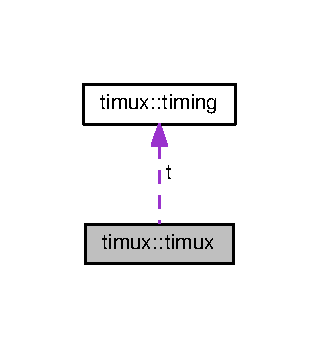
\includegraphics[width=153pt]{classtimux_1_1timux__coll__graph}
\end{center}
\end{figure}
\subsection*{Public Member Functions}
\begin{DoxyCompactItemize}
\item 
void \hyperlink{classtimux_1_1timux_ac732153dc6019d7ddd3aa93fdffcfc6f}{recived} (\hyperlink{structtimux_1_1msg}{msg} $\ast$m)
\item 
\hyperlink{classtimux_1_1timux_a84e972805455951e68973856c91d8bb4}{timux} (\hyperlink{classllu_1_1network_1_1_managed_connection}{llu\+::network\+::\+Managed\+Connection} $\ast$con, unsigned long \hyperlink{classtimux_1_1timux_aac1a2022c0fc41f5ce690f40037af2cf}{frame\+Length}, unsigned long \hyperlink{classtimux_1_1timux_a3c8195dcabf2a776759b09f66e08bc80}{slot\+Count}, sockaddr\+\_\+in target)
\item 
void \hyperlink{classtimux_1_1timux_aedd4f1380074ca99661aa8ba142d5b72}{loop} ()
\end{DoxyCompactItemize}
\subsection*{Public Attributes}
\begin{DoxyCompactItemize}
\item 
\hyperlink{classtimux_1_1timing}{timing} \hyperlink{classtimux_1_1timux_a880a260ad67a47cbdbbd756a42ea0e48}{t}
\item 
unsigned long \hyperlink{classtimux_1_1timux_aac1a2022c0fc41f5ce690f40037af2cf}{frame\+Length}
\item 
unsigned long \hyperlink{classtimux_1_1timux_a3c8195dcabf2a776759b09f66e08bc80}{slot\+Count}
\end{DoxyCompactItemize}


\subsection{Detailed Description}
the main Class that performess all the logic 

Definition at line 78 of file timux.\+hpp.



\subsection{Constructor \& Destructor Documentation}
\hypertarget{classtimux_1_1timux_a84e972805455951e68973856c91d8bb4}{\index{timux\+::timux@{timux\+::timux}!timux@{timux}}
\index{timux@{timux}!timux\+::timux@{timux\+::timux}}
\subsubsection[{timux}]{\setlength{\rightskip}{0pt plus 5cm}timux\+::timux\+::timux (
\begin{DoxyParamCaption}
\item[{{\bf llu\+::network\+::\+Managed\+Connection} $\ast$}]{con, }
\item[{unsigned long}]{frame\+Length, }
\item[{unsigned long}]{slot\+Count, }
\item[{sockaddr\+\_\+in}]{target}
\end{DoxyParamCaption}
)}}\label{classtimux_1_1timux_a84e972805455951e68973856c91d8bb4}


Definition at line 65 of file timux.\+cpp.



\subsection{Member Function Documentation}
\hypertarget{classtimux_1_1timux_aedd4f1380074ca99661aa8ba142d5b72}{\index{timux\+::timux@{timux\+::timux}!loop@{loop}}
\index{loop@{loop}!timux\+::timux@{timux\+::timux}}
\subsubsection[{loop}]{\setlength{\rightskip}{0pt plus 5cm}void timux\+::timux\+::loop (
\begin{DoxyParamCaption}
{}
\end{DoxyParamCaption}
)}}\label{classtimux_1_1timux_aedd4f1380074ca99661aa8ba142d5b72}


Definition at line 121 of file timux.\+cpp.

\hypertarget{classtimux_1_1timux_ac732153dc6019d7ddd3aa93fdffcfc6f}{\index{timux\+::timux@{timux\+::timux}!recived@{recived}}
\index{recived@{recived}!timux\+::timux@{timux\+::timux}}
\subsubsection[{recived}]{\setlength{\rightskip}{0pt plus 5cm}void timux\+::timux\+::recived (
\begin{DoxyParamCaption}
\item[{{\bf msg} $\ast$}]{m}
\end{DoxyParamCaption}
)}}\label{classtimux_1_1timux_ac732153dc6019d7ddd3aa93fdffcfc6f}


Definition at line 91 of file timux.\+cpp.



\subsection{Member Data Documentation}
\hypertarget{classtimux_1_1timux_aac1a2022c0fc41f5ce690f40037af2cf}{\index{timux\+::timux@{timux\+::timux}!frame\+Length@{frame\+Length}}
\index{frame\+Length@{frame\+Length}!timux\+::timux@{timux\+::timux}}
\subsubsection[{frame\+Length}]{\setlength{\rightskip}{0pt plus 5cm}unsigned long timux\+::timux\+::frame\+Length}}\label{classtimux_1_1timux_aac1a2022c0fc41f5ce690f40037af2cf}


Definition at line 123 of file timux.\+hpp.

\hypertarget{classtimux_1_1timux_a3c8195dcabf2a776759b09f66e08bc80}{\index{timux\+::timux@{timux\+::timux}!slot\+Count@{slot\+Count}}
\index{slot\+Count@{slot\+Count}!timux\+::timux@{timux\+::timux}}
\subsubsection[{slot\+Count}]{\setlength{\rightskip}{0pt plus 5cm}unsigned long timux\+::timux\+::slot\+Count}}\label{classtimux_1_1timux_a3c8195dcabf2a776759b09f66e08bc80}


Definition at line 124 of file timux.\+hpp.

\hypertarget{classtimux_1_1timux_a880a260ad67a47cbdbbd756a42ea0e48}{\index{timux\+::timux@{timux\+::timux}!t@{t}}
\index{t@{t}!timux\+::timux@{timux\+::timux}}
\subsubsection[{t}]{\setlength{\rightskip}{0pt plus 5cm}{\bf timing} timux\+::timux\+::t}}\label{classtimux_1_1timux_a880a260ad67a47cbdbbd756a42ea0e48}


Definition at line 122 of file timux.\+hpp.



The documentation for this class was generated from the following files\+:\begin{DoxyCompactItemize}
\item 
time\+Mux/\hyperlink{timux_8hpp}{timux.\+hpp}\item 
time\+Mux/\hyperlink{timux_8cpp}{timux.\+cpp}\end{DoxyCompactItemize}

\hypertarget{classllu_1_1network_1_1_udp_connection}{\section{llu\+:\+:network\+:\+:Udp\+Connection Class Reference}
\label{classllu_1_1network_1_1_udp_connection}\index{llu\+::network\+::\+Udp\+Connection@{llu\+::network\+::\+Udp\+Connection}}
}


{\ttfamily \#include $<$udp.\+hpp$>$}



Inheritance diagram for llu\+:\+:network\+:\+:Udp\+Connection\+:
\nopagebreak
\begin{figure}[H]
\begin{center}
\leavevmode
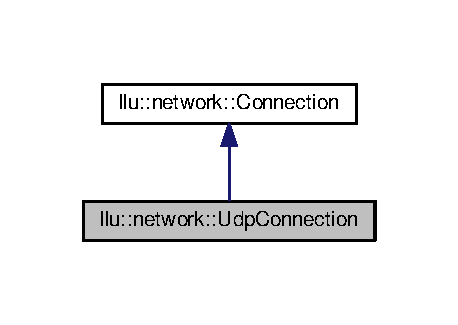
\includegraphics[width=220pt]{classllu_1_1network_1_1_udp_connection__inherit__graph}
\end{center}
\end{figure}


Collaboration diagram for llu\+:\+:network\+:\+:Udp\+Connection\+:
\nopagebreak
\begin{figure}[H]
\begin{center}
\leavevmode
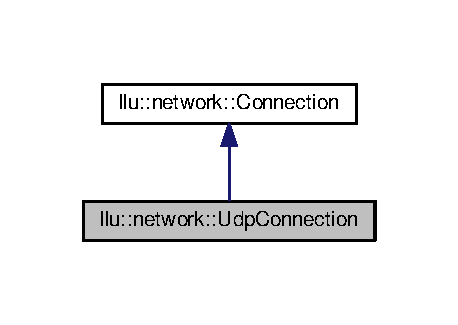
\includegraphics[width=220pt]{classllu_1_1network_1_1_udp_connection__coll__graph}
\end{center}
\end{figure}
\subsection*{Public Member Functions}
\begin{DoxyCompactItemize}
\item 
\hyperlink{classllu_1_1network_1_1_udp_connection_a715f5dabf94e43a9a54385a647cc587b}{Udp\+Connection} (char ttl=1, uint16\+\_\+t my\+Port=0, size\+\_\+t max\+Rcv\+Msg\+Leng=128)
\item 
\hyperlink{structllu_1_1network_1_1recived_message}{recived\+Message} $\ast$ \hyperlink{classllu_1_1network_1_1_udp_connection_abbd9d3906a283f5506a69a8922fa76c6}{recv\+Msg} ()
\begin{DoxyCompactList}\small\item\em recives a \hyperlink{structllu_1_1network_1_1recived_message}{recived\+Message} from the connection \end{DoxyCompactList}\item 
void \hyperlink{classllu_1_1network_1_1_udp_connection_a044432ee61191ecabd295fe4ea6cddf1}{send\+Msg} (\hyperlink{structllu_1_1network_1_1send_message}{send\+Message} $\ast$m)
\begin{DoxyCompactList}\small\item\em sends the message m over the \hyperlink{classllu_1_1network_1_1_connection}{Connection} \end{DoxyCompactList}\item 
bool \hyperlink{classllu_1_1network_1_1_udp_connection_add200cb20d4ece925b8752675d375828}{alive} ()
\begin{DoxyCompactList}\small\item\em used to check if the connection is usable \end{DoxyCompactList}\item 
void \hyperlink{classllu_1_1network_1_1_udp_connection_a97a62c2ab3975d9716f965aacc2f28fc}{kill} ()
\begin{DoxyCompactList}\small\item\em closes a connection \end{DoxyCompactList}\end{DoxyCompactItemize}


\subsection{Detailed Description}


Definition at line 23 of file udp.\+hpp.



\subsection{Constructor \& Destructor Documentation}
\hypertarget{classllu_1_1network_1_1_udp_connection_a715f5dabf94e43a9a54385a647cc587b}{\index{llu\+::network\+::\+Udp\+Connection@{llu\+::network\+::\+Udp\+Connection}!Udp\+Connection@{Udp\+Connection}}
\index{Udp\+Connection@{Udp\+Connection}!llu\+::network\+::\+Udp\+Connection@{llu\+::network\+::\+Udp\+Connection}}
\subsubsection[{Udp\+Connection}]{\setlength{\rightskip}{0pt plus 5cm}llu\+::network\+::\+Udp\+Connection\+::\+Udp\+Connection (
\begin{DoxyParamCaption}
\item[{char}]{ttl = {\ttfamily 1}, }
\item[{uint16\+\_\+t}]{my\+Port = {\ttfamily 0}, }
\item[{size\+\_\+t}]{max\+Rcv\+Msg\+Leng = {\ttfamily 128}}
\end{DoxyParamCaption}
)}}\label{classllu_1_1network_1_1_udp_connection_a715f5dabf94e43a9a54385a647cc587b}


Definition at line 12 of file udp.\+cpp.



\subsection{Member Function Documentation}
\hypertarget{classllu_1_1network_1_1_udp_connection_add200cb20d4ece925b8752675d375828}{\index{llu\+::network\+::\+Udp\+Connection@{llu\+::network\+::\+Udp\+Connection}!alive@{alive}}
\index{alive@{alive}!llu\+::network\+::\+Udp\+Connection@{llu\+::network\+::\+Udp\+Connection}}
\subsubsection[{alive}]{\setlength{\rightskip}{0pt plus 5cm}bool llu\+::network\+::\+Udp\+Connection\+::alive (
\begin{DoxyParamCaption}
{}
\end{DoxyParamCaption}
)\hspace{0.3cm}{\ttfamily [virtual]}}}\label{classllu_1_1network_1_1_udp_connection_add200cb20d4ece925b8752675d375828}


used to check if the connection is usable 

\begin{DoxyReturn}{Returns}
true if usable, otherwise false 
\end{DoxyReturn}


Implements \hyperlink{classllu_1_1network_1_1_connection_a05893a11a26ea97663637cf085e1b985}{llu\+::network\+::\+Connection}.



Definition at line 42 of file udp.\+cpp.

\hypertarget{classllu_1_1network_1_1_udp_connection_a97a62c2ab3975d9716f965aacc2f28fc}{\index{llu\+::network\+::\+Udp\+Connection@{llu\+::network\+::\+Udp\+Connection}!kill@{kill}}
\index{kill@{kill}!llu\+::network\+::\+Udp\+Connection@{llu\+::network\+::\+Udp\+Connection}}
\subsubsection[{kill}]{\setlength{\rightskip}{0pt plus 5cm}void llu\+::network\+::\+Udp\+Connection\+::kill (
\begin{DoxyParamCaption}
{}
\end{DoxyParamCaption}
)\hspace{0.3cm}{\ttfamily [virtual]}}}\label{classllu_1_1network_1_1_udp_connection_a97a62c2ab3975d9716f965aacc2f28fc}


closes a connection 



Implements \hyperlink{classllu_1_1network_1_1_connection_a7e620755dde598fffc96d3ee6b3326a1}{llu\+::network\+::\+Connection}.



Definition at line 46 of file udp.\+cpp.

\hypertarget{classllu_1_1network_1_1_udp_connection_abbd9d3906a283f5506a69a8922fa76c6}{\index{llu\+::network\+::\+Udp\+Connection@{llu\+::network\+::\+Udp\+Connection}!recv\+Msg@{recv\+Msg}}
\index{recv\+Msg@{recv\+Msg}!llu\+::network\+::\+Udp\+Connection@{llu\+::network\+::\+Udp\+Connection}}
\subsubsection[{recv\+Msg}]{\setlength{\rightskip}{0pt plus 5cm}{\bf recived\+Message} $\ast$ llu\+::network\+::\+Udp\+Connection\+::recv\+Msg (
\begin{DoxyParamCaption}
{}
\end{DoxyParamCaption}
)\hspace{0.3cm}{\ttfamily [virtual]}}}\label{classllu_1_1network_1_1_udp_connection_abbd9d3906a283f5506a69a8922fa76c6}


recives a \hyperlink{structllu_1_1network_1_1recived_message}{recived\+Message} from the connection 

Blocks untill data is avaliable \begin{DoxyReturn}{Returns}
the \hyperlink{structllu_1_1network_1_1recived_message}{recived\+Message} rescived the responsebilety for the result belonges to the caller 
\end{DoxyReturn}


Implements \hyperlink{classllu_1_1network_1_1_connection_aae606f5aad246e892db5665cd7be1747}{llu\+::network\+::\+Connection}.



Definition at line 28 of file udp.\+cpp.

\hypertarget{classllu_1_1network_1_1_udp_connection_a044432ee61191ecabd295fe4ea6cddf1}{\index{llu\+::network\+::\+Udp\+Connection@{llu\+::network\+::\+Udp\+Connection}!send\+Msg@{send\+Msg}}
\index{send\+Msg@{send\+Msg}!llu\+::network\+::\+Udp\+Connection@{llu\+::network\+::\+Udp\+Connection}}
\subsubsection[{send\+Msg}]{\setlength{\rightskip}{0pt plus 5cm}void llu\+::network\+::\+Udp\+Connection\+::send\+Msg (
\begin{DoxyParamCaption}
\item[{{\bf send\+Message} $\ast$}]{m}
\end{DoxyParamCaption}
)\hspace{0.3cm}{\ttfamily [virtual]}}}\label{classllu_1_1network_1_1_udp_connection_a044432ee61191ecabd295fe4ea6cddf1}


sends the message m over the \hyperlink{classllu_1_1network_1_1_connection}{Connection} 

this methode is not blocking m will be deletet using destory\+Send\+Message 

Implements \hyperlink{classllu_1_1network_1_1_connection_ac20ca6d4d56b39fadde27b6af10000ae}{llu\+::network\+::\+Connection}.



Definition at line 36 of file udp.\+cpp.



The documentation for this class was generated from the following files\+:\begin{DoxyCompactItemize}
\item 
time\+Mux/\hyperlink{udp_8hpp}{udp.\+hpp}\item 
time\+Mux/\hyperlink{udp_8cpp}{udp.\+cpp}\end{DoxyCompactItemize}

\chapter{File Documentation}
\hypertarget{bc_server_8cpp}{\section{time\+Mux/bc\+Server.cpp File Reference}
\label{bc_server_8cpp}\index{time\+Mux/bc\+Server.\+cpp@{time\+Mux/bc\+Server.\+cpp}}
}


Implementation of a U\+D\+P Broadcast server for testing.  


{\ttfamily \#include $<$iostream$>$}\\*
{\ttfamily \#include \char`\"{}callback.\+hpp\char`\"{}}\\*
{\ttfamily \#include \char`\"{}ring\+Buffer.\+hpp\char`\"{}}\\*
{\ttfamily \#include \char`\"{}udp.\+hpp\char`\"{}}\\*
{\ttfamily \#include $<$chrono$>$}\\*
{\ttfamily \#include $<$thread$>$}\\*
{\ttfamily \#include $<$netinet/in.\+h$>$}\\*
{\ttfamily \#include $<$arpa/inet.\+h$>$}\\*
{\ttfamily \#include $<$mutex$>$}\\*
Include dependency graph for bc\+Server.\+cpp\+:
\nopagebreak
\begin{figure}[H]
\begin{center}
\leavevmode
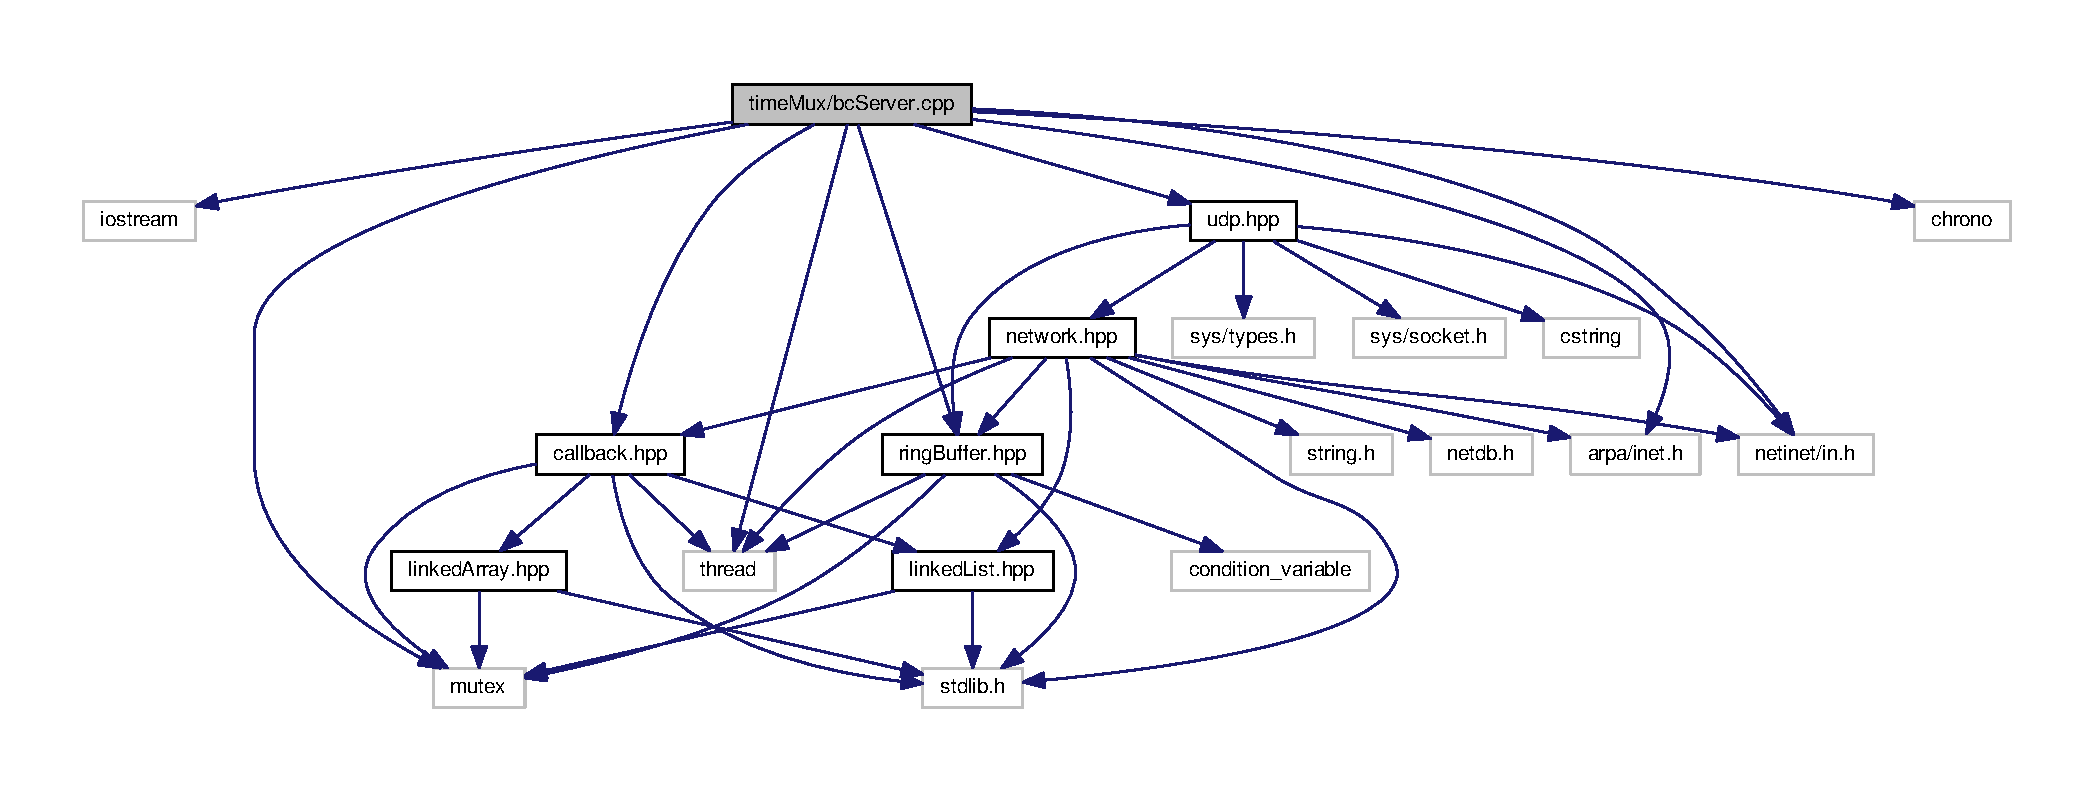
\includegraphics[width=350pt]{bc_server_8cpp__incl}
\end{center}
\end{figure}
\subsection*{Macros}
\begin{DoxyCompactItemize}
\item 
\#define \hyperlink{bc_server_8cpp_a158a930828d856b72962ae4bb14d79a7}{E\+C\+H\+O\+\_\+\+S\+I\+G\+N\+A\+L}~(1)
\end{DoxyCompactItemize}
\subsection*{Functions}
\begin{DoxyCompactItemize}
\item 
bool \hyperlink{bc_server_8cpp_a73b04ffa1af0870539b2176ccd5fc1f3}{Print\+Matcher} (\hyperlink{structllu_1_1network_1_1recived_message}{recived\+Message} $\ast$m, \hyperlink{namespacellu_1_1callback_a082ed24306809c4d250bd5ddfbae177f}{signal} $\ast$s)
\item 
void \hyperlink{bc_server_8cpp_a17110670e7e47fbc3d08946d2891f8db}{Print\+Handler} (void $\ast$c, \hyperlink{structllu_1_1network_1_1recived_message}{recived\+Message} $\ast$m)
\item 
bool \hyperlink{bc_server_8cpp_ae915c722df9438586415bb59a2a7cbce}{socketaddr\+Compare} (sockaddr\+\_\+in A, sockaddr\+\_\+in B)
\item 
void \hyperlink{bc_server_8cpp_a2dc45723754eab307e0b3ce87735309d}{B\+C\+Handler} (void $\ast$c, \hyperlink{structllu_1_1network_1_1recived_message}{recived\+Message} $\ast$m)
\item 
int \hyperlink{bc_server_8cpp_ae66f6b31b5ad750f1fe042a706a4e3d4}{main} ()
\end{DoxyCompactItemize}
\subsection*{Variables}
\begin{DoxyCompactItemize}
\item 
mutex \hyperlink{bc_server_8cpp_ab68c2cee22ffb1d6c7829af1ff88f95a}{screen\+Lock}
\item 
\hyperlink{classllu_1_1datastructs_1_1_linked_list}{Linked\+List}$<$ sockaddr\+\_\+in $>$ \hyperlink{bc_server_8cpp_acce8f31ca286e21002e779752b8b218a}{client\+List}
\item 
mutex \hyperlink{bc_server_8cpp_aeeac01e4649111607f78ca1cc033f067}{list\+Lock}
\end{DoxyCompactItemize}


\subsection{Detailed Description}
Implementation of a U\+D\+P Broadcast server for testing. 

\begin{DoxyAuthor}{Author}
Lukas Lühr (hexagon2206) 
\end{DoxyAuthor}
\begin{DoxyRefDesc}{Bug}
\item[\hyperlink{bug__bug000001}{Bug}]No known bugs. \end{DoxyRefDesc}


Definition in file \hyperlink{bc_server_8cpp_source}{bc\+Server.\+cpp}.



\subsection{Macro Definition Documentation}
\hypertarget{bc_server_8cpp_a158a930828d856b72962ae4bb14d79a7}{\index{bc\+Server.\+cpp@{bc\+Server.\+cpp}!E\+C\+H\+O\+\_\+\+S\+I\+G\+N\+A\+L@{E\+C\+H\+O\+\_\+\+S\+I\+G\+N\+A\+L}}
\index{E\+C\+H\+O\+\_\+\+S\+I\+G\+N\+A\+L@{E\+C\+H\+O\+\_\+\+S\+I\+G\+N\+A\+L}!bc\+Server.\+cpp@{bc\+Server.\+cpp}}
\subsubsection[{E\+C\+H\+O\+\_\+\+S\+I\+G\+N\+A\+L}]{\setlength{\rightskip}{0pt plus 5cm}\#define E\+C\+H\+O\+\_\+\+S\+I\+G\+N\+A\+L~(1)}}\label{bc_server_8cpp_a158a930828d856b72962ae4bb14d79a7}


Definition at line 23 of file bc\+Server.\+cpp.



\subsection{Function Documentation}
\hypertarget{bc_server_8cpp_a2dc45723754eab307e0b3ce87735309d}{\index{bc\+Server.\+cpp@{bc\+Server.\+cpp}!B\+C\+Handler@{B\+C\+Handler}}
\index{B\+C\+Handler@{B\+C\+Handler}!bc\+Server.\+cpp@{bc\+Server.\+cpp}}
\subsubsection[{B\+C\+Handler}]{\setlength{\rightskip}{0pt plus 5cm}void B\+C\+Handler (
\begin{DoxyParamCaption}
\item[{void $\ast$}]{c, }
\item[{{\bf recived\+Message} $\ast$}]{m}
\end{DoxyParamCaption}
)}}\label{bc_server_8cpp_a2dc45723754eab307e0b3ce87735309d}


Definition at line 47 of file bc\+Server.\+cpp.

\hypertarget{bc_server_8cpp_ae66f6b31b5ad750f1fe042a706a4e3d4}{\index{bc\+Server.\+cpp@{bc\+Server.\+cpp}!main@{main}}
\index{main@{main}!bc\+Server.\+cpp@{bc\+Server.\+cpp}}
\subsubsection[{main}]{\setlength{\rightskip}{0pt plus 5cm}int main (
\begin{DoxyParamCaption}
{}
\end{DoxyParamCaption}
)}}\label{bc_server_8cpp_ae66f6b31b5ad750f1fe042a706a4e3d4}


Definition at line 69 of file bc\+Server.\+cpp.

\hypertarget{bc_server_8cpp_a17110670e7e47fbc3d08946d2891f8db}{\index{bc\+Server.\+cpp@{bc\+Server.\+cpp}!Print\+Handler@{Print\+Handler}}
\index{Print\+Handler@{Print\+Handler}!bc\+Server.\+cpp@{bc\+Server.\+cpp}}
\subsubsection[{Print\+Handler}]{\setlength{\rightskip}{0pt plus 5cm}void Print\+Handler (
\begin{DoxyParamCaption}
\item[{void $\ast$}]{c, }
\item[{{\bf recived\+Message} $\ast$}]{m}
\end{DoxyParamCaption}
)}}\label{bc_server_8cpp_a17110670e7e47fbc3d08946d2891f8db}


Definition at line 30 of file bc\+Server.\+cpp.

\hypertarget{bc_server_8cpp_a73b04ffa1af0870539b2176ccd5fc1f3}{\index{bc\+Server.\+cpp@{bc\+Server.\+cpp}!Print\+Matcher@{Print\+Matcher}}
\index{Print\+Matcher@{Print\+Matcher}!bc\+Server.\+cpp@{bc\+Server.\+cpp}}
\subsubsection[{Print\+Matcher}]{\setlength{\rightskip}{0pt plus 5cm}bool Print\+Matcher (
\begin{DoxyParamCaption}
\item[{{\bf recived\+Message} $\ast$}]{m, }
\item[{{\bf signal} $\ast$}]{s}
\end{DoxyParamCaption}
)}}\label{bc_server_8cpp_a73b04ffa1af0870539b2176ccd5fc1f3}


Definition at line 24 of file bc\+Server.\+cpp.

\hypertarget{bc_server_8cpp_ae915c722df9438586415bb59a2a7cbce}{\index{bc\+Server.\+cpp@{bc\+Server.\+cpp}!socketaddr\+Compare@{socketaddr\+Compare}}
\index{socketaddr\+Compare@{socketaddr\+Compare}!bc\+Server.\+cpp@{bc\+Server.\+cpp}}
\subsubsection[{socketaddr\+Compare}]{\setlength{\rightskip}{0pt plus 5cm}bool socketaddr\+Compare (
\begin{DoxyParamCaption}
\item[{sockaddr\+\_\+in}]{A, }
\item[{sockaddr\+\_\+in}]{B}
\end{DoxyParamCaption}
)}}\label{bc_server_8cpp_ae915c722df9438586415bb59a2a7cbce}


Definition at line 41 of file bc\+Server.\+cpp.



\subsection{Variable Documentation}
\hypertarget{bc_server_8cpp_acce8f31ca286e21002e779752b8b218a}{\index{bc\+Server.\+cpp@{bc\+Server.\+cpp}!client\+List@{client\+List}}
\index{client\+List@{client\+List}!bc\+Server.\+cpp@{bc\+Server.\+cpp}}
\subsubsection[{client\+List}]{\setlength{\rightskip}{0pt plus 5cm}{\bf Linked\+List}$<$sockaddr\+\_\+in$>$ client\+List}}\label{bc_server_8cpp_acce8f31ca286e21002e779752b8b218a}


Definition at line 44 of file bc\+Server.\+cpp.

\hypertarget{bc_server_8cpp_aeeac01e4649111607f78ca1cc033f067}{\index{bc\+Server.\+cpp@{bc\+Server.\+cpp}!list\+Lock@{list\+Lock}}
\index{list\+Lock@{list\+Lock}!bc\+Server.\+cpp@{bc\+Server.\+cpp}}
\subsubsection[{list\+Lock}]{\setlength{\rightskip}{0pt plus 5cm}mutex list\+Lock}}\label{bc_server_8cpp_aeeac01e4649111607f78ca1cc033f067}


Definition at line 45 of file bc\+Server.\+cpp.

\hypertarget{bc_server_8cpp_ab68c2cee22ffb1d6c7829af1ff88f95a}{\index{bc\+Server.\+cpp@{bc\+Server.\+cpp}!screen\+Lock@{screen\+Lock}}
\index{screen\+Lock@{screen\+Lock}!bc\+Server.\+cpp@{bc\+Server.\+cpp}}
\subsubsection[{screen\+Lock}]{\setlength{\rightskip}{0pt plus 5cm}mutex screen\+Lock}}\label{bc_server_8cpp_ab68c2cee22ffb1d6c7829af1ff88f95a}


Definition at line 29 of file bc\+Server.\+cpp.


\hypertarget{callback_8cpp}{\section{time\+Mux/callback.cpp File Reference}
\label{callback_8cpp}\index{time\+Mux/callback.\+cpp@{time\+Mux/callback.\+cpp}}
}
{\ttfamily \#include \char`\"{}callback.\+hpp\char`\"{}}\\*
Include dependency graph for callback.\+cpp\+:
\nopagebreak
\begin{figure}[H]
\begin{center}
\leavevmode
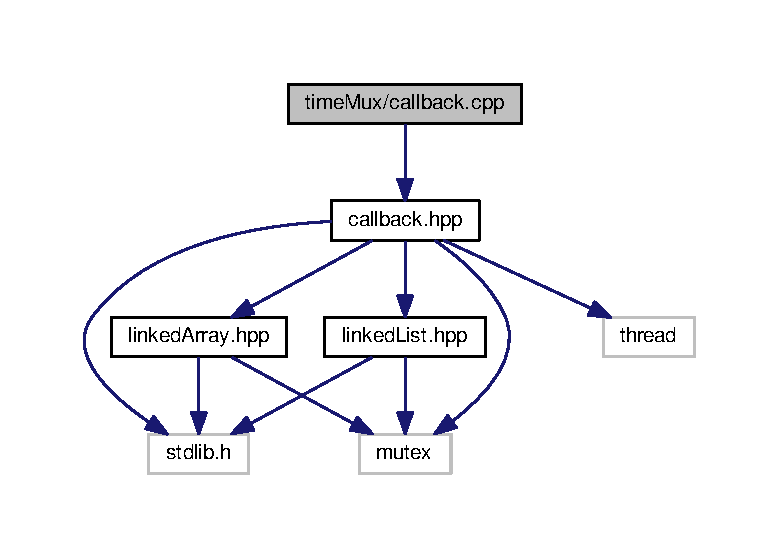
\includegraphics[width=350pt]{callback_8cpp__incl}
\end{center}
\end{figure}
\subsection*{Namespaces}
\begin{DoxyCompactItemize}
\item 
 \hyperlink{namespacellu}{llu}
\item 
 \hyperlink{namespacellu_1_1callback}{llu\+::callback}
\begin{DoxyCompactList}\small\item\em Contains the implementation of a generik callback handler. \end{DoxyCompactList}\end{DoxyCompactItemize}

\hypertarget{callback_8hpp}{\section{time\+Mux/callback.hpp File Reference}
\label{callback_8hpp}\index{time\+Mux/callback.\+hpp@{time\+Mux/callback.\+hpp}}
}


Prototypes for a Callback Handler.  


{\ttfamily \#include $<$stdlib.\+h$>$}\\*
{\ttfamily \#include $<$thread$>$}\\*
{\ttfamily \#include $<$mutex$>$}\\*
{\ttfamily \#include \char`\"{}linked\+List.\+hpp\char`\"{}}\\*
{\ttfamily \#include \char`\"{}linked\+Array.\+hpp\char`\"{}}\\*
Include dependency graph for callback.\+hpp\+:
\nopagebreak
\begin{figure}[H]
\begin{center}
\leavevmode
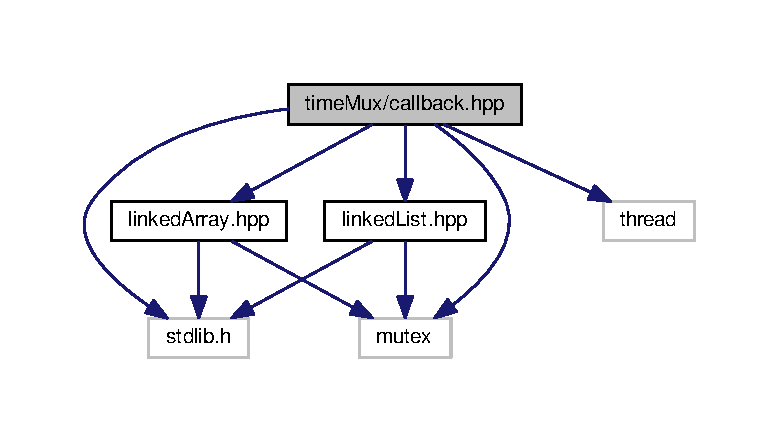
\includegraphics[width=350pt]{callback_8hpp__incl}
\end{center}
\end{figure}
This graph shows which files directly or indirectly include this file\+:
\nopagebreak
\begin{figure}[H]
\begin{center}
\leavevmode
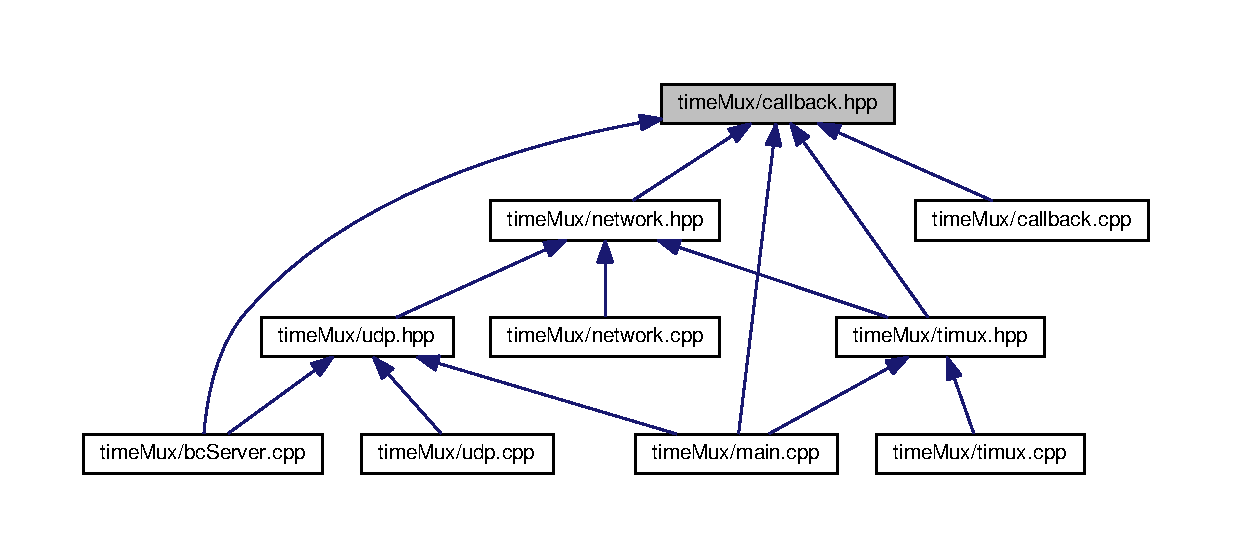
\includegraphics[width=350pt]{callback_8hpp__dep__incl}
\end{center}
\end{figure}
\subsection*{Classes}
\begin{DoxyCompactItemize}
\item 
class \hyperlink{classllu_1_1callback_1_1callback__registration}{llu\+::callback\+::callback\+\_\+registration$<$ C, D $>$}
\begin{DoxyCompactList}\small\item\em Calback registration, containing functon and. \end{DoxyCompactList}\item 
class \hyperlink{classllu_1_1callback_1_1_callback}{llu\+::callback\+::\+Callback$<$ C, D $>$}
\begin{DoxyCompactList}\small\item\em Calback manager class. \end{DoxyCompactList}\end{DoxyCompactItemize}
\subsection*{Namespaces}
\begin{DoxyCompactItemize}
\item 
 \hyperlink{namespacellu}{llu}
\item 
 \hyperlink{namespacellu_1_1callback}{llu\+::callback}
\begin{DoxyCompactList}\small\item\em Contains the implementation of a generik callback handler. \end{DoxyCompactList}\end{DoxyCompactItemize}
\subsection*{Typedefs}
\begin{DoxyCompactItemize}
\item 
typedef unsigned int \hyperlink{namespacellu_1_1callback_a082ed24306809c4d250bd5ddfbae177f}{llu\+::callback\+::signal}
\end{DoxyCompactItemize}


\subsection{Detailed Description}
Prototypes for a Callback Handler. 

\begin{DoxyAuthor}{Author}
Lukas Lühr (hexagon2206) 
\end{DoxyAuthor}
\begin{DoxyRefDesc}{Bug}
\item[\hyperlink{bug__bug000002}{Bug}]No known bugs. \end{DoxyRefDesc}


Definition in file \hyperlink{callback_8hpp_source}{callback.\+hpp}.


\hypertarget{docs_8hpp}{\section{time\+Mux/docs.hpp File Reference}
\label{docs_8hpp}\index{time\+Mux/docs.\+hpp@{time\+Mux/docs.\+hpp}}
}


Namespace Documenation header.  


\subsection*{Namespaces}
\begin{DoxyCompactItemize}
\item 
 \hyperlink{namespacellu}{llu}
\item 
 \hyperlink{namespacellu_1_1datastructs}{llu\+::datastructs}
\begin{DoxyCompactList}\small\item\em Contains som generik data structures like ring buffer oder linked list. \end{DoxyCompactList}\item 
 \hyperlink{namespacellu_1_1callback}{llu\+::callback}
\begin{DoxyCompactList}\small\item\em Contains the implementation of a generik callback handler. \end{DoxyCompactList}\item 
 \hyperlink{namespacellu_1_1network}{llu\+::network}
\begin{DoxyCompactList}\small\item\em Contaions functionalety used for network komunikation. \end{DoxyCompactList}\end{DoxyCompactItemize}


\subsection{Detailed Description}
Namespace Documenation header. 

\begin{DoxyAuthor}{Author}
Lukas Lühr (hexagon2206) 
\end{DoxyAuthor}


Definition in file \hyperlink{docs_8hpp_source}{docs.\+hpp}.


\hypertarget{linked_array_8hpp}{\section{time\+Mux/linked\+Array.hpp File Reference}
\label{linked_array_8hpp}\index{time\+Mux/linked\+Array.\+hpp@{time\+Mux/linked\+Array.\+hpp}}
}


Prototypes for a Linked Array. The Linked array implements acces over simulated index in a linked list.  


{\ttfamily \#include $<$stdlib.\+h$>$}\\*
{\ttfamily \#include $<$mutex$>$}\\*
Include dependency graph for linked\+Array.\+hpp\+:
\nopagebreak
\begin{figure}[H]
\begin{center}
\leavevmode
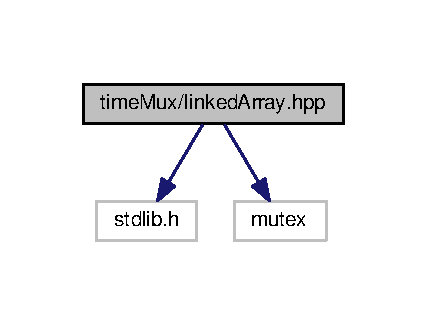
\includegraphics[width=205pt]{linked_array_8hpp__incl}
\end{center}
\end{figure}
This graph shows which files directly or indirectly include this file\+:
\nopagebreak
\begin{figure}[H]
\begin{center}
\leavevmode
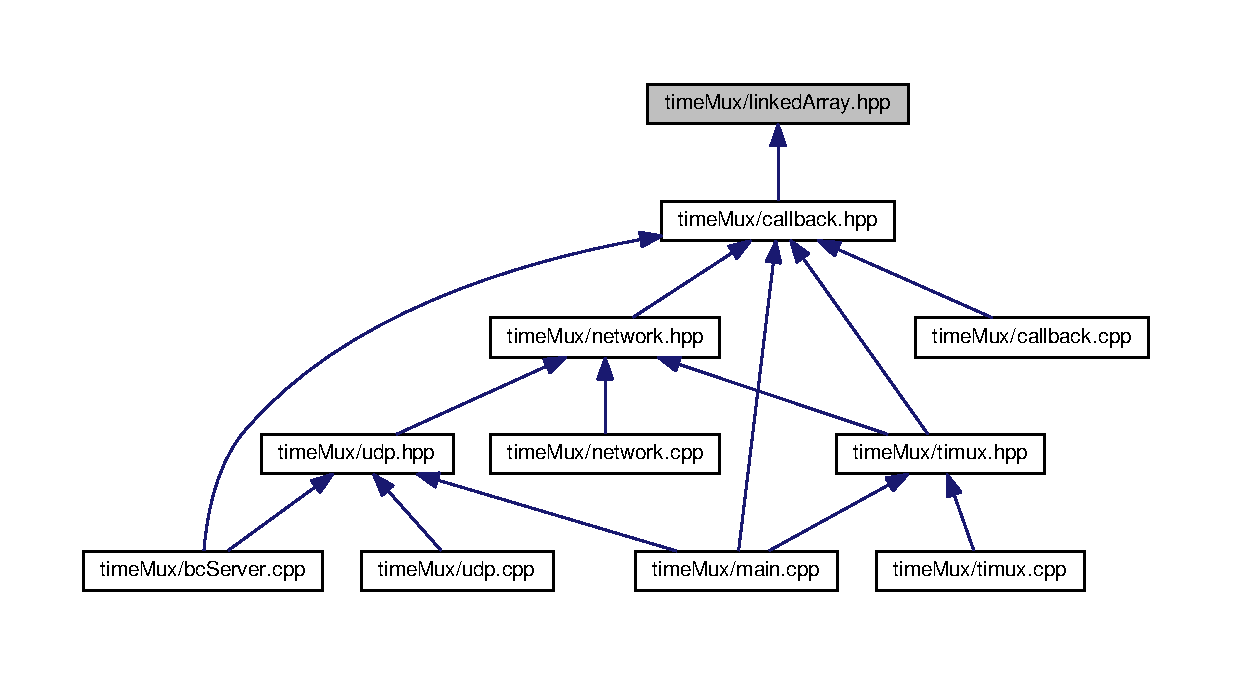
\includegraphics[width=350pt]{linked_array_8hpp__dep__incl}
\end{center}
\end{figure}
\subsection*{Classes}
\begin{DoxyCompactItemize}
\item 
struct \hyperlink{structllu_1_1datastructs_1_1list_array_entrie}{llu\+::datastructs\+::list\+Array\+Entrie$<$ E $>$}
\begin{DoxyCompactList}\small\item\em An entry of an list\+Array of type E. \end{DoxyCompactList}\item 
class \hyperlink{classllu_1_1datastructs_1_1_linked_list_array}{llu\+::datastructs\+::\+Linked\+List\+Array$<$ E $>$}
\begin{DoxyCompactList}\small\item\em Implementation of a simple generik thread save Array. \end{DoxyCompactList}\end{DoxyCompactItemize}
\subsection*{Namespaces}
\begin{DoxyCompactItemize}
\item 
 \hyperlink{namespacellu}{llu}
\item 
 \hyperlink{namespacellu_1_1datastructs}{llu\+::datastructs}
\begin{DoxyCompactList}\small\item\em Contains som generik data structures like ring buffer oder linked list. \end{DoxyCompactList}\end{DoxyCompactItemize}


\subsection{Detailed Description}
Prototypes for a Linked Array. The Linked array implements acces over simulated index in a linked list. 

\begin{DoxyAuthor}{Author}
Lukas Lühr (hexagon2206) 
\end{DoxyAuthor}
\begin{DoxyRefDesc}{Bug}
\item[\hyperlink{bug__bug000003}{Bug}]No known bugs. \end{DoxyRefDesc}


Definition in file \hyperlink{linked_array_8hpp_source}{linked\+Array.\+hpp}.


\hypertarget{linked_list_8hpp}{\section{time\+Mux/linked\+List.hpp File Reference}
\label{linked_list_8hpp}\index{time\+Mux/linked\+List.\+hpp@{time\+Mux/linked\+List.\+hpp}}
}


implements a generik Linked List.  


{\ttfamily \#include $<$stdlib.\+h$>$}\\*
{\ttfamily \#include $<$mutex$>$}\\*
Include dependency graph for linked\+List.\+hpp\+:
\nopagebreak
\begin{figure}[H]
\begin{center}
\leavevmode
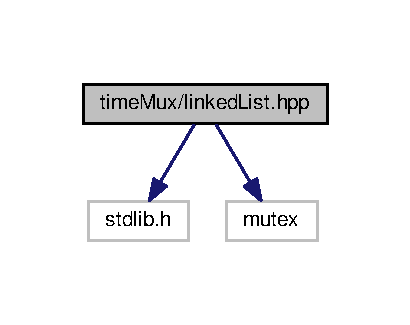
\includegraphics[width=197pt]{linked_list_8hpp__incl}
\end{center}
\end{figure}
This graph shows which files directly or indirectly include this file\+:
\nopagebreak
\begin{figure}[H]
\begin{center}
\leavevmode
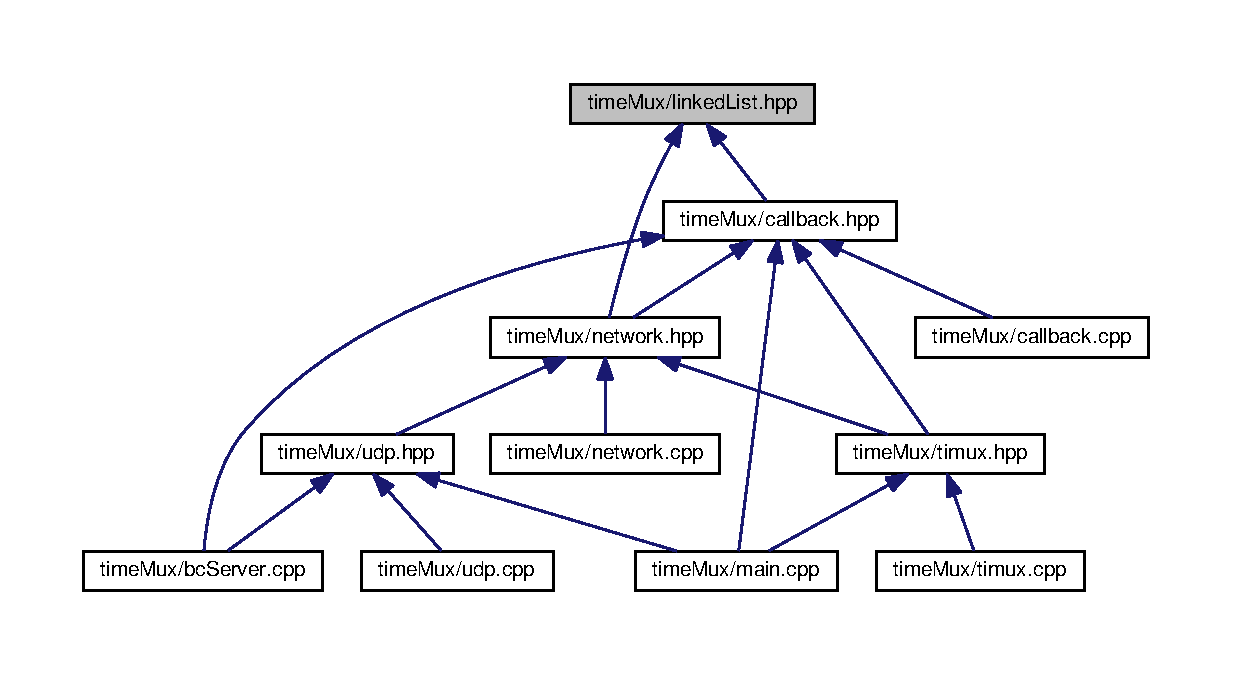
\includegraphics[width=350pt]{linked_list_8hpp__dep__incl}
\end{center}
\end{figure}
\subsection*{Classes}
\begin{DoxyCompactItemize}
\item 
struct \hyperlink{structllu_1_1datastructs_1_1list_entrie}{llu\+::datastructs\+::list\+Entrie$<$ E $>$}
\begin{DoxyCompactList}\small\item\em an list entry for a linked list of type E \end{DoxyCompactList}\item 
class \hyperlink{classllu_1_1datastructs_1_1_linked_list}{llu\+::datastructs\+::\+Linked\+List$<$ E $>$}
\begin{DoxyCompactList}\small\item\em very spartanic implementation of a generik thread save Linked list \end{DoxyCompactList}\end{DoxyCompactItemize}
\subsection*{Namespaces}
\begin{DoxyCompactItemize}
\item 
 \hyperlink{namespacellu}{llu}
\item 
 \hyperlink{namespacellu_1_1datastructs}{llu\+::datastructs}
\begin{DoxyCompactList}\small\item\em Contains som generik data structures like ring buffer oder linked list. \end{DoxyCompactList}\end{DoxyCompactItemize}


\subsection{Detailed Description}
implements a generik Linked List. 

\begin{DoxyAuthor}{Author}
Lukas Lühr (hexagon2206) 
\end{DoxyAuthor}
\begin{DoxyRefDesc}{Bug}
\item[\hyperlink{bug__bug000004}{Bug}]No known bugs. \end{DoxyRefDesc}


Definition in file \hyperlink{linked_list_8hpp_source}{linked\+List.\+hpp}.


\hypertarget{main_8cpp}{\section{time\+Mux/main.cpp File Reference}
\label{main_8cpp}\index{time\+Mux/main.\+cpp@{time\+Mux/main.\+cpp}}
}


Startsup the Timux System.  


{\ttfamily \#include $<$iostream$>$}\\*
{\ttfamily \#include \char`\"{}callback.\+hpp\char`\"{}}\\*
{\ttfamily \#include \char`\"{}ring\+Buffer.\+hpp\char`\"{}}\\*
{\ttfamily \#include \char`\"{}udp.\+hpp\char`\"{}}\\*
{\ttfamily \#include $<$chrono$>$}\\*
{\ttfamily \#include $<$thread$>$}\\*
{\ttfamily \#include $<$netinet/in.\+h$>$}\\*
{\ttfamily \#include $<$arpa/inet.\+h$>$}\\*
{\ttfamily \#include $<$time.\+h$>$}\\*
{\ttfamily \#include $<$mutex$>$}\\*
{\ttfamily \#include \char`\"{}timux.\+hpp\char`\"{}}\\*
Include dependency graph for main.\+cpp\+:
\nopagebreak
\begin{figure}[H]
\begin{center}
\leavevmode
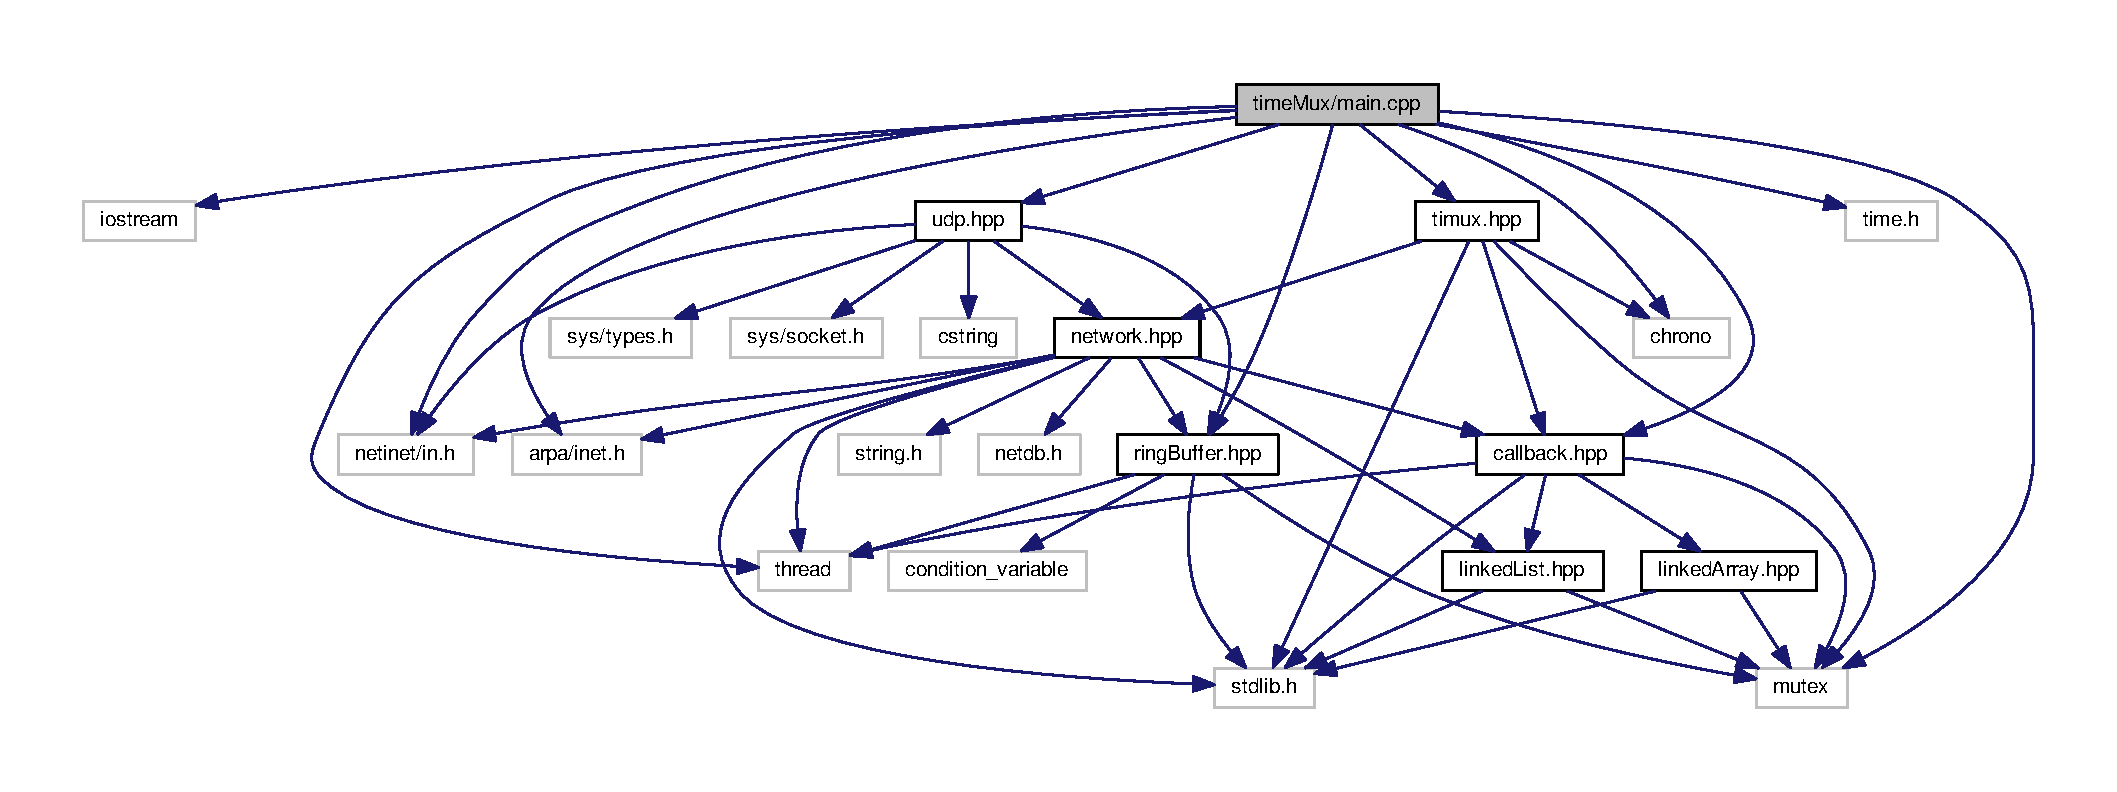
\includegraphics[width=350pt]{main_8cpp__incl}
\end{center}
\end{figure}
\subsection*{Functions}
\begin{DoxyCompactItemize}
\item 
int \hyperlink{main_8cpp_ae66f6b31b5ad750f1fe042a706a4e3d4}{main} ()
\end{DoxyCompactItemize}


\subsection{Detailed Description}
Startsup the Timux System. 

\begin{DoxyAuthor}{Author}
Lukas Lühr (hexagon2206) 
\end{DoxyAuthor}
\begin{DoxyRefDesc}{Bug}
\item[\hyperlink{bug__bug000005}{Bug}]No known bugs. \end{DoxyRefDesc}


Definition in file \hyperlink{main_8cpp_source}{main.\+cpp}.



\subsection{Function Documentation}
\hypertarget{main_8cpp_ae66f6b31b5ad750f1fe042a706a4e3d4}{\index{main.\+cpp@{main.\+cpp}!main@{main}}
\index{main@{main}!main.\+cpp@{main.\+cpp}}
\subsubsection[{main}]{\setlength{\rightskip}{0pt plus 5cm}int main (
\begin{DoxyParamCaption}
{}
\end{DoxyParamCaption}
)}}\label{main_8cpp_ae66f6b31b5ad750f1fe042a706a4e3d4}


Definition at line 30 of file main.\+cpp.


\hypertarget{network_8cpp}{\section{time\+Mux/network.cpp File Reference}
\label{network_8cpp}\index{time\+Mux/network.\+cpp@{time\+Mux/network.\+cpp}}
}


Implementation of al general network stuff.  


{\ttfamily \#include \char`\"{}network.\+hpp\char`\"{}}\\*
Include dependency graph for network.\+cpp\+:
\nopagebreak
\begin{figure}[H]
\begin{center}
\leavevmode
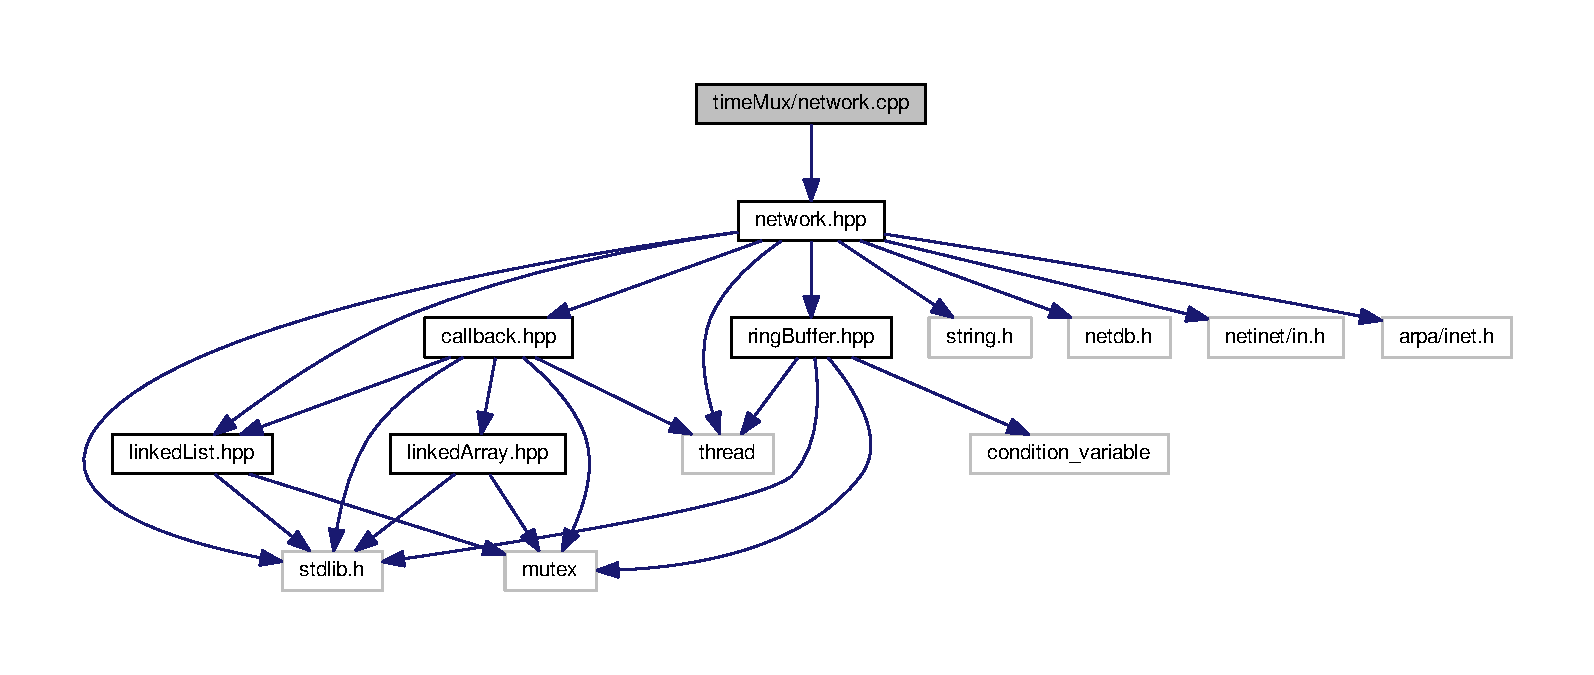
\includegraphics[width=350pt]{network_8cpp__incl}
\end{center}
\end{figure}
\subsection*{Namespaces}
\begin{DoxyCompactItemize}
\item 
 \hyperlink{namespacellu}{llu}
\item 
 \hyperlink{namespacellu_1_1network}{llu\+::network}
\begin{DoxyCompactList}\small\item\em Contaions functionalety used for network komunikation. \end{DoxyCompactList}\end{DoxyCompactItemize}
\subsection*{Functions}
\begin{DoxyCompactItemize}
\item 
void \hyperlink{namespacellu_1_1network_a9db735ab1f182142c349fc313e33c32d}{llu\+::network\+::to\+N\+B\+O} (uint8\+\_\+t value, uint8\+\_\+t $\ast$target)
\begin{DoxyCompactList}\small\item\em convertes a given value to the Network byte order (big endian) \end{DoxyCompactList}\item 
uint8\+\_\+t \hyperlink{namespacellu_1_1network_aec38b31ea6f294a14c7c3f9e426b312d}{llu\+::network\+::to\+H\+B\+O\+\_\+8} (uint8\+\_\+t $\ast$from)
\begin{DoxyCompactList}\small\item\em convertes a given byte fiedl in Network byte order to host byte order \end{DoxyCompactList}\item 
void \hyperlink{namespacellu_1_1network_aa1dd1b9198bfbe8d3fd01ca358d8d538}{llu\+::network\+::to\+N\+B\+O} (uint16\+\_\+t value, uint8\+\_\+t $\ast$target)
\begin{DoxyCompactList}\small\item\em convertes a given value to the Network byte order (big endian) \end{DoxyCompactList}\item 
uint16\+\_\+t \hyperlink{namespacellu_1_1network_a6c358826dbd0c43ec751139dca87ab71}{llu\+::network\+::to\+H\+B\+O\+\_\+16} (uint8\+\_\+t $\ast$from)
\begin{DoxyCompactList}\small\item\em convertes a given byte fiedl in Network byte order to host byte order \end{DoxyCompactList}\item 
void \hyperlink{namespacellu_1_1network_a0132a9cde9b08a16e9b05709ea16a2b9}{llu\+::network\+::to\+N\+B\+O} (uint32\+\_\+t value, uint8\+\_\+t $\ast$target)
\begin{DoxyCompactList}\small\item\em convertes a given value to the Network byte order (big endian) \end{DoxyCompactList}\item 
uint32\+\_\+t \hyperlink{namespacellu_1_1network_a2222539df59075cc6f892b12956968eb}{llu\+::network\+::to\+H\+B\+O\+\_\+32} (uint8\+\_\+t $\ast$from)
\begin{DoxyCompactList}\small\item\em convertes a given byte fiedl in Network byte order to host byte order \end{DoxyCompactList}\item 
void \hyperlink{namespacellu_1_1network_af0b046f65433995d5150c3f8251e7d07}{llu\+::network\+::to\+N\+B\+O} (uint64\+\_\+t value, uint8\+\_\+t $\ast$target)
\begin{DoxyCompactList}\small\item\em convertes a given value to the Network byte order (big endian) \end{DoxyCompactList}\item 
uint64\+\_\+t \hyperlink{namespacellu_1_1network_af97d326c7853fc1b5932a56b8cc8e4b6}{llu\+::network\+::to\+H\+B\+O\+\_\+64} (uint8\+\_\+t $\ast$from)
\begin{DoxyCompactList}\small\item\em convertes a given byte fiedl in Network byte order to host byte order \end{DoxyCompactList}\item 
sockaddr\+\_\+in \hyperlink{namespacellu_1_1network_ae50fed51b566b947fd0cb1a4efbb3b12}{llu\+::network\+::resolve} (const char $\ast$addr, uint16\+\_\+t port)
\begin{DoxyCompactList}\small\item\em resolves an Ipv4 and an port to a sockaddr\+\_\+in \end{DoxyCompactList}\item 
recived\+Message $\ast$ \hyperlink{namespacellu_1_1network_a867a402a3f2a945cf6d5f9b9c9ca4bd1}{llu\+::network\+::create\+Recived\+Message} (size\+\_\+t buffer\+Size)
\begin{DoxyCompactList}\small\item\em creates an empry \hyperlink{structllu_1_1network_1_1recived_message}{recived\+Message} object \end{DoxyCompactList}\item 
void \hyperlink{namespacellu_1_1network_a957314727976f73a1566322ad0229ca8}{llu\+::network\+::destory\+Recived\+Message} (recived\+Message $\ast$m)
\begin{DoxyCompactList}\small\item\em deletes a recived Massage, the data field itself is not touched \end{DoxyCompactList}\item 
send\+Message $\ast$ \hyperlink{namespacellu_1_1network_a86501a24323e339aa0a3b4e935bb2495}{llu\+::network\+::create\+Send\+Message} (size\+\_\+t buffer\+Size, sockaddr\+\_\+in target, const void $\ast$from)
\begin{DoxyCompactList}\small\item\em creates a Message ready to be send to a connection \end{DoxyCompactList}\item 
void \hyperlink{namespacellu_1_1network_a8c61905bb65d88aa69349ee7138577a8}{llu\+::network\+::destory\+Send\+Message} (send\+Message $\ast$m)
\begin{DoxyCompactList}\small\item\em deletes a send Massage, the data field itself is not touched \end{DoxyCompactList}\item 
recived\+Message $\ast$ \hyperlink{namespacellu_1_1network_a126aeba4f63e2f7d5617ee4568b32895}{llu\+::network\+::copy\+Recived\+Message} (recived\+Message $\ast$r)
\begin{DoxyCompactList}\small\item\em copies an compleate \hyperlink{structllu_1_1network_1_1recived_message}{recived\+Message} \end{DoxyCompactList}\end{DoxyCompactItemize}


\subsection{Detailed Description}
Implementation of al general network stuff. 

\begin{DoxyAuthor}{Author}
Lukas Lühr (hexagon2206) 
\end{DoxyAuthor}
\begin{DoxyRefDesc}{Bug}
\item[\hyperlink{bug__bug000006}{Bug}]No known bugs. \end{DoxyRefDesc}


Definition in file \hyperlink{network_8cpp_source}{network.\+cpp}.


\hypertarget{network_8hpp}{\section{time\+Mux/network.hpp File Reference}
\label{network_8hpp}\index{time\+Mux/network.\+hpp@{time\+Mux/network.\+hpp}}
}


Prototypes for network comunikation.  


{\ttfamily \#include $<$stdlib.\+h$>$}\\*
{\ttfamily \#include $<$string.\+h$>$}\\*
{\ttfamily \#include $<$thread$>$}\\*
{\ttfamily \#include $<$netdb.\+h$>$}\\*
{\ttfamily \#include $<$netinet/in.\+h$>$}\\*
{\ttfamily \#include $<$arpa/inet.\+h$>$}\\*
{\ttfamily \#include \char`\"{}callback.\+hpp\char`\"{}}\\*
{\ttfamily \#include \char`\"{}ring\+Buffer.\+hpp\char`\"{}}\\*
{\ttfamily \#include \char`\"{}linked\+List.\+hpp\char`\"{}}\\*
Include dependency graph for network.\+hpp\+:
\nopagebreak
\begin{figure}[H]
\begin{center}
\leavevmode
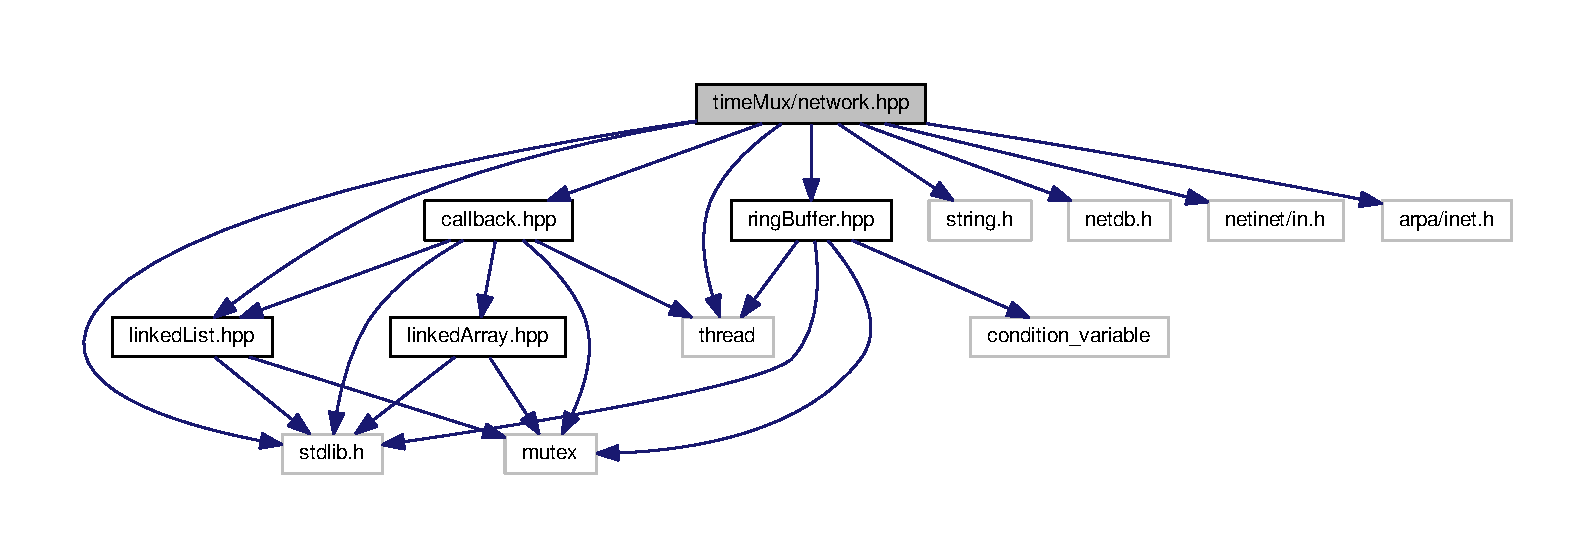
\includegraphics[width=350pt]{network_8hpp__incl}
\end{center}
\end{figure}
This graph shows which files directly or indirectly include this file\+:
\nopagebreak
\begin{figure}[H]
\begin{center}
\leavevmode
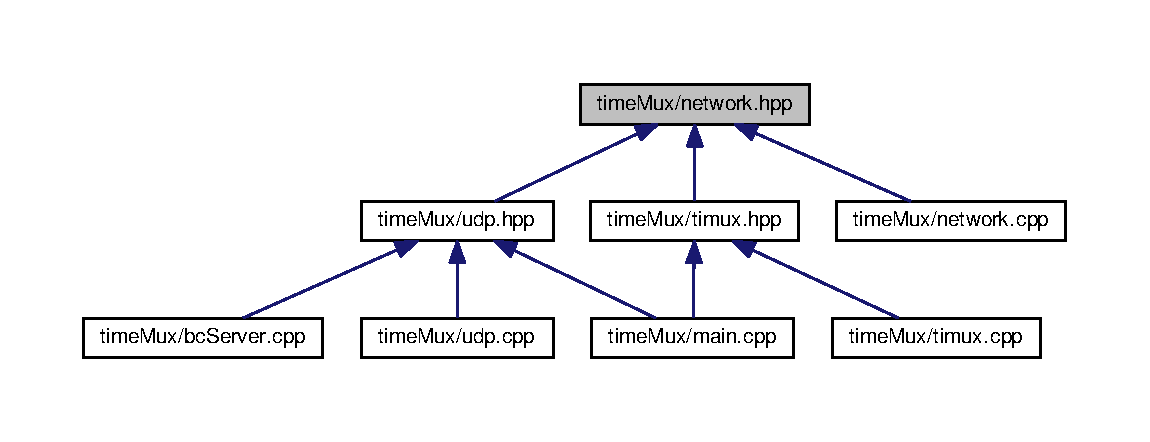
\includegraphics[width=350pt]{network_8hpp__dep__incl}
\end{center}
\end{figure}
\subsection*{Classes}
\begin{DoxyCompactItemize}
\item 
struct \hyperlink{structllu_1_1network_1_1recived_message}{llu\+::network\+::recived\+Message}
\begin{DoxyCompactList}\small\item\em an recived message from an \hyperlink{classllu_1_1network_1_1_connection}{Connection} object \end{DoxyCompactList}\item 
struct \hyperlink{structllu_1_1network_1_1send_message}{llu\+::network\+::send\+Message}
\begin{DoxyCompactList}\small\item\em A message ready to be send. \end{DoxyCompactList}\item 
class \hyperlink{classllu_1_1network_1_1_connection}{llu\+::network\+::\+Connection}
\item 
class \hyperlink{classllu_1_1network_1_1_managed_connection}{llu\+::network\+::\+Managed\+Connection}
\begin{DoxyCompactList}\small\item\em a Managed form of a \hyperlink{classllu_1_1network_1_1_connection}{Connection} implements callbacks on massage recive internayls uses a callback handler \end{DoxyCompactList}\end{DoxyCompactItemize}
\subsection*{Namespaces}
\begin{DoxyCompactItemize}
\item 
 \hyperlink{namespacellu}{llu}
\item 
 \hyperlink{namespacellu_1_1network}{llu\+::network}
\begin{DoxyCompactList}\small\item\em Contaions functionalety used for network komunikation. \end{DoxyCompactList}\end{DoxyCompactItemize}
\subsection*{Typedefs}
\begin{DoxyCompactItemize}
\item 
typedef bool( \hyperlink{namespacellu_1_1network_a62e69230f04d1998f17b11e3bcc2d121}{llu\+::network\+::recived\+Message\+Classifier\+Type} )(recived\+Message $\ast$, \hyperlink{namespacellu_1_1callback_a082ed24306809c4d250bd5ddfbae177f}{signal} $\ast$)
\begin{DoxyCompactList}\small\item\em a Classifiere for massages recived Messages, the type \end{DoxyCompactList}\item 
typedef \\*
recived\+Message\+Classifier\+Type $\ast$ \hyperlink{namespacellu_1_1network_ac629c1180a0bee8ddef541f73cb3e5f9}{llu\+::network\+::recived\+Message\+Classifier}
\begin{DoxyCompactList}\small\item\em the classifier pointer \end{DoxyCompactList}\item 
typedef \hyperlink{classllu_1_1callback_1_1callback__registration}{callback\+\_\+registration}\\*
$<$ void $\ast$, recived\+Message $\ast$ $>$ \hyperlink{namespacellu_1_1network_a999d34263abe84a87d12271383c606b9}{llu\+::network\+::netwok\+Msg\+Callback}
\begin{DoxyCompactList}\small\item\em an callback registration for a mannaged connection \end{DoxyCompactList}\end{DoxyCompactItemize}
\subsection*{Functions}
\begin{DoxyCompactItemize}
\item 
void \hyperlink{namespacellu_1_1network_a9db735ab1f182142c349fc313e33c32d}{llu\+::network\+::to\+N\+B\+O} (uint8\+\_\+t value, uint8\+\_\+t $\ast$target)
\begin{DoxyCompactList}\small\item\em convertes a given value to the Network byte order (big endian) \end{DoxyCompactList}\item 
uint8\+\_\+t \hyperlink{namespacellu_1_1network_aec38b31ea6f294a14c7c3f9e426b312d}{llu\+::network\+::to\+H\+B\+O\+\_\+8} (uint8\+\_\+t $\ast$from)
\begin{DoxyCompactList}\small\item\em convertes a given byte fiedl in Network byte order to host byte order \end{DoxyCompactList}\item 
void \hyperlink{namespacellu_1_1network_aa1dd1b9198bfbe8d3fd01ca358d8d538}{llu\+::network\+::to\+N\+B\+O} (uint16\+\_\+t value, uint8\+\_\+t $\ast$target)
\begin{DoxyCompactList}\small\item\em convertes a given value to the Network byte order (big endian) \end{DoxyCompactList}\item 
uint16\+\_\+t \hyperlink{namespacellu_1_1network_a6c358826dbd0c43ec751139dca87ab71}{llu\+::network\+::to\+H\+B\+O\+\_\+16} (uint8\+\_\+t $\ast$from)
\begin{DoxyCompactList}\small\item\em convertes a given byte fiedl in Network byte order to host byte order \end{DoxyCompactList}\item 
void \hyperlink{namespacellu_1_1network_a0132a9cde9b08a16e9b05709ea16a2b9}{llu\+::network\+::to\+N\+B\+O} (uint32\+\_\+t value, uint8\+\_\+t $\ast$target)
\begin{DoxyCompactList}\small\item\em convertes a given value to the Network byte order (big endian) \end{DoxyCompactList}\item 
uint32\+\_\+t \hyperlink{namespacellu_1_1network_a2222539df59075cc6f892b12956968eb}{llu\+::network\+::to\+H\+B\+O\+\_\+32} (uint8\+\_\+t $\ast$from)
\begin{DoxyCompactList}\small\item\em convertes a given byte fiedl in Network byte order to host byte order \end{DoxyCompactList}\item 
void \hyperlink{namespacellu_1_1network_af0b046f65433995d5150c3f8251e7d07}{llu\+::network\+::to\+N\+B\+O} (uint64\+\_\+t value, uint8\+\_\+t $\ast$target)
\begin{DoxyCompactList}\small\item\em convertes a given value to the Network byte order (big endian) \end{DoxyCompactList}\item 
uint64\+\_\+t \hyperlink{namespacellu_1_1network_af97d326c7853fc1b5932a56b8cc8e4b6}{llu\+::network\+::to\+H\+B\+O\+\_\+64} (uint8\+\_\+t $\ast$from)
\begin{DoxyCompactList}\small\item\em convertes a given byte fiedl in Network byte order to host byte order \end{DoxyCompactList}\item 
sockaddr\+\_\+in \hyperlink{namespacellu_1_1network_ae50fed51b566b947fd0cb1a4efbb3b12}{llu\+::network\+::resolve} (const char $\ast$addr, uint16\+\_\+t port)
\begin{DoxyCompactList}\small\item\em resolves an Ipv4 and an port to a sockaddr\+\_\+in \end{DoxyCompactList}\item 
recived\+Message $\ast$ \hyperlink{namespacellu_1_1network_a867a402a3f2a945cf6d5f9b9c9ca4bd1}{llu\+::network\+::create\+Recived\+Message} (size\+\_\+t buffer\+Size)
\begin{DoxyCompactList}\small\item\em creates an empry \hyperlink{structllu_1_1network_1_1recived_message}{recived\+Message} object \end{DoxyCompactList}\item 
void \hyperlink{namespacellu_1_1network_a957314727976f73a1566322ad0229ca8}{llu\+::network\+::destory\+Recived\+Message} (recived\+Message $\ast$m)
\begin{DoxyCompactList}\small\item\em deletes a recived Massage, the data field itself is not touched \end{DoxyCompactList}\item 
send\+Message $\ast$ \hyperlink{namespacellu_1_1network_a86501a24323e339aa0a3b4e935bb2495}{llu\+::network\+::create\+Send\+Message} (size\+\_\+t buffer\+Size, sockaddr\+\_\+in target, const void $\ast$from)
\begin{DoxyCompactList}\small\item\em creates a Message ready to be send to a connection \end{DoxyCompactList}\item 
void \hyperlink{namespacellu_1_1network_a8c61905bb65d88aa69349ee7138577a8}{llu\+::network\+::destory\+Send\+Message} (send\+Message $\ast$m)
\begin{DoxyCompactList}\small\item\em deletes a send Massage, the data field itself is not touched \end{DoxyCompactList}\item 
recived\+Message $\ast$ \hyperlink{namespacellu_1_1network_a126aeba4f63e2f7d5617ee4568b32895}{llu\+::network\+::copy\+Recived\+Message} (recived\+Message $\ast$r)
\begin{DoxyCompactList}\small\item\em copies an compleate \hyperlink{structllu_1_1network_1_1recived_message}{recived\+Message} \end{DoxyCompactList}\end{DoxyCompactItemize}


\subsection{Detailed Description}
Prototypes for network comunikation. 

\begin{DoxyAuthor}{Author}
Lukas Lühr (hexagon2206) 
\end{DoxyAuthor}
\begin{DoxyRefDesc}{Bug}
\item[\hyperlink{bug__bug000007}{Bug}]No known bugs. \end{DoxyRefDesc}


Definition in file \hyperlink{network_8hpp_source}{network.\+hpp}.


\hypertarget{ring_buffer_8hpp}{\section{time\+Mux/ring\+Buffer.hpp File Reference}
\label{ring_buffer_8hpp}\index{time\+Mux/ring\+Buffer.\+hpp@{time\+Mux/ring\+Buffer.\+hpp}}
}


Impelemnts a generik Ging buffer.  


{\ttfamily \#include $<$stdlib.\+h$>$}\\*
{\ttfamily \#include $<$condition\+\_\+variable$>$}\\*
{\ttfamily \#include $<$thread$>$}\\*
{\ttfamily \#include $<$mutex$>$}\\*
Include dependency graph for ring\+Buffer.\+hpp\+:
\nopagebreak
\begin{figure}[H]
\begin{center}
\leavevmode
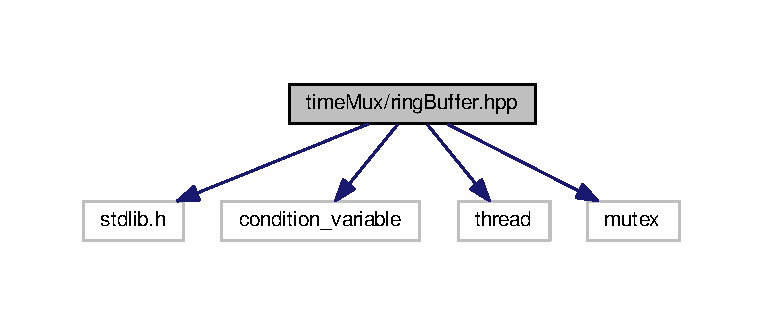
\includegraphics[width=350pt]{ring_buffer_8hpp__incl}
\end{center}
\end{figure}
This graph shows which files directly or indirectly include this file\+:
\nopagebreak
\begin{figure}[H]
\begin{center}
\leavevmode
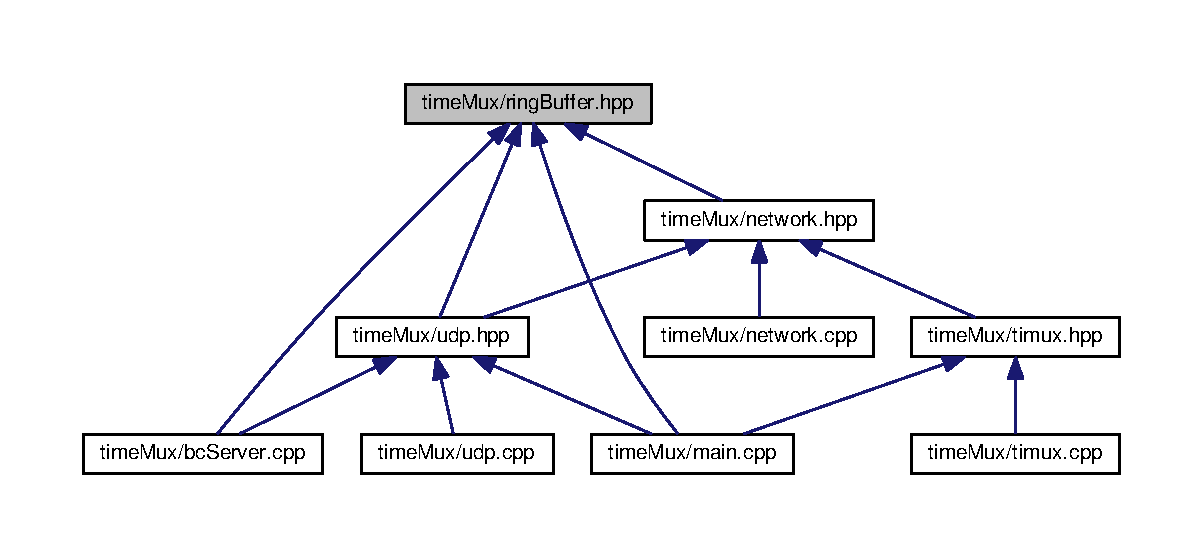
\includegraphics[width=350pt]{ring_buffer_8hpp__dep__incl}
\end{center}
\end{figure}
\subsection*{Classes}
\begin{DoxyCompactItemize}
\item 
class \hyperlink{classllu_1_1datastructs_1_1_ringbuffer}{llu\+::datastructs\+::\+Ringbuffer$<$ D $>$}
\begin{DoxyCompactList}\small\item\em Basic implementation of a generik and thread save Ring buffer. \end{DoxyCompactList}\end{DoxyCompactItemize}
\subsection*{Namespaces}
\begin{DoxyCompactItemize}
\item 
 \hyperlink{namespacellu}{llu}
\item 
 \hyperlink{namespacellu_1_1datastructs}{llu\+::datastructs}
\begin{DoxyCompactList}\small\item\em Contains som generik data structures like ring buffer oder linked list. \end{DoxyCompactList}\end{DoxyCompactItemize}


\subsection{Detailed Description}
Impelemnts a generik Ging buffer. 

\begin{DoxyAuthor}{Author}
Lukas Lühr (hexagon2206) 
\end{DoxyAuthor}
\begin{DoxyRefDesc}{Bug}
\item[\hyperlink{bug__bug000008}{Bug}]No known bugs. \end{DoxyRefDesc}


Definition in file \hyperlink{ring_buffer_8hpp_source}{ring\+Buffer.\+hpp}.


\hypertarget{timux_8cpp}{\section{time\+Mux/timux.cpp File Reference}
\label{timux_8cpp}\index{time\+Mux/timux.\+cpp@{time\+Mux/timux.\+cpp}}
}


Implementation of The T\+I\+M\+U\+X logic.  


{\ttfamily \#include \char`\"{}timux.\+hpp\char`\"{}}\\*
{\ttfamily \#include $<$iostream$>$}\\*
Include dependency graph for timux.\+cpp\+:
\nopagebreak
\begin{figure}[H]
\begin{center}
\leavevmode
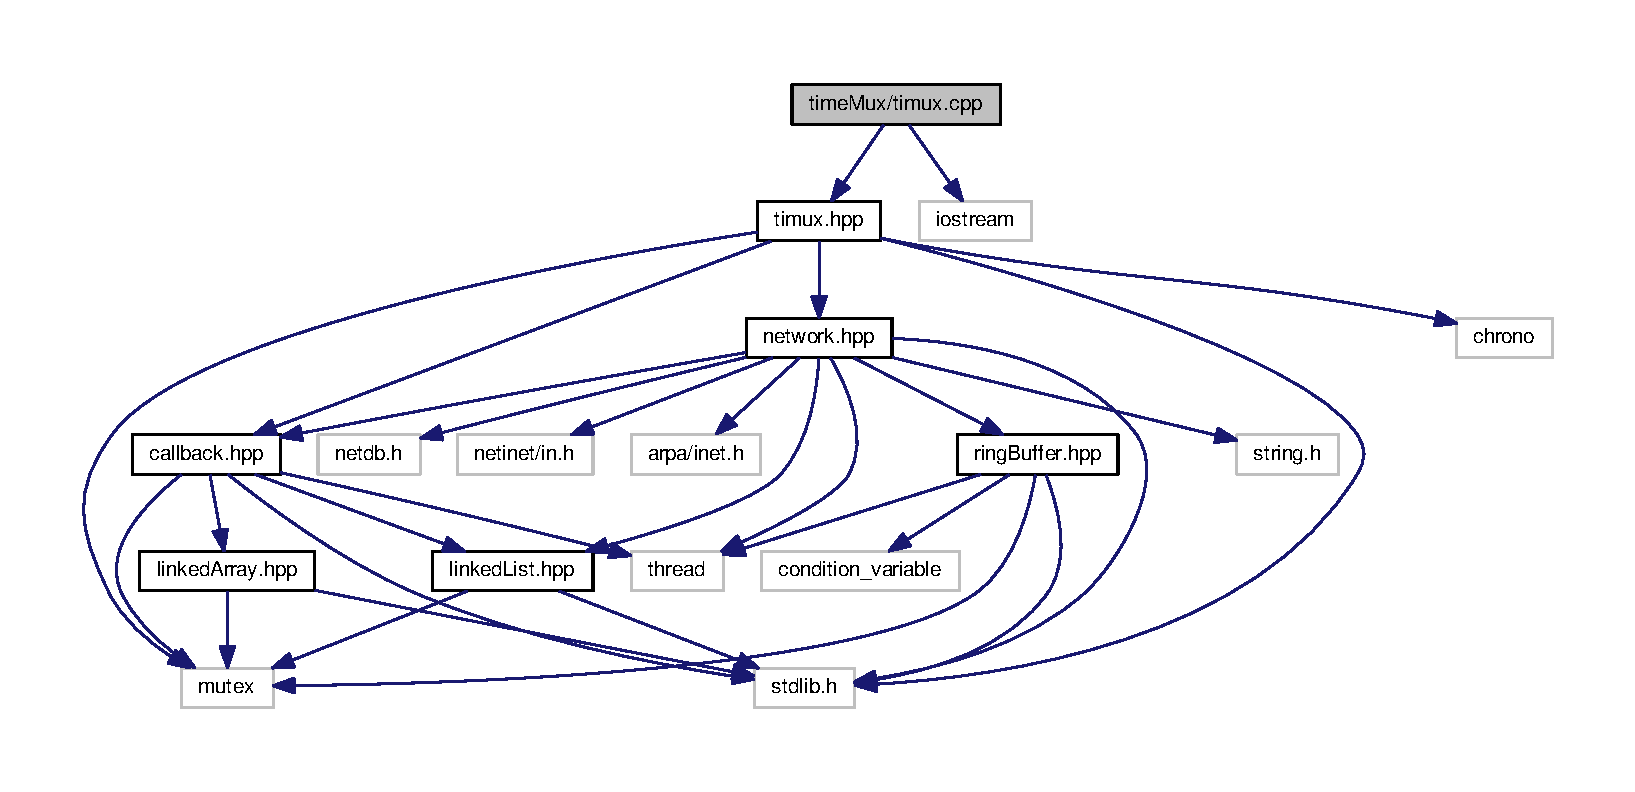
\includegraphics[width=350pt]{timux_8cpp__incl}
\end{center}
\end{figure}
\subsection*{Namespaces}
\begin{DoxyCompactItemize}
\item 
 \hyperlink{namespacetimux}{timux}
\end{DoxyCompactItemize}
\subsection*{Macros}
\begin{DoxyCompactItemize}
\item 
\#define \hyperlink{timux_8cpp_aef41e8aaf4c60819b30faf396cdf4978}{D\+E\+B\+U\+G}(X)
\end{DoxyCompactItemize}
\subsection*{Functions}
\begin{DoxyCompactItemize}
\item 
bool \hyperlink{namespacetimux_af9d865eb949c95b170ca458395332f06}{timux\+::\+Time\+Synchronize\+Signal} (\hyperlink{structllu_1_1network_1_1recived_message}{llu\+::network\+::recived\+Message} $\ast$m, \hyperlink{namespacellu_1_1callback_a082ed24306809c4d250bd5ddfbae177f}{llu\+::callback\+::signal} $\ast$s)
\begin{DoxyCompactList}\small\item\em signals a T\+I\+M\+U\+X\+\_\+\+Time\+Signal , if the gven message m is from an A-\/\+Station \end{DoxyCompactList}\item 
void \hyperlink{namespacetimux_aaaa8c2d5485d4108b450aa5edf1e3aa3}{timux\+::\+Time\+Synchronize\+Handler} (void $\ast$timing\+Class, \hyperlink{structllu_1_1network_1_1recived_message}{llu\+::network\+::recived\+Message} $\ast$m)
\begin{DoxyCompactList}\small\item\em adjusts the offset of a timing class \end{DoxyCompactList}\item 
bool \hyperlink{namespacetimux_ad0edf69fd830fa995ad603731acd5a20}{timux\+::\+Msg\+Signal} (\hyperlink{structllu_1_1network_1_1recived_message}{llu\+::network\+::recived\+Message} $\ast$m, \hyperlink{namespacellu_1_1callback_a082ed24306809c4d250bd5ddfbae177f}{llu\+::callback\+::signal} $\ast$s)
\begin{DoxyCompactList}\small\item\em signals a T\+I\+M\+U\+X\+\_\+\+Sot\+Signal if a message is recived \end{DoxyCompactList}\item 
void \hyperlink{namespacetimux_a0325847c7fd72e51034fc14c8547d505}{timux\+::\+Msg\+Handler} (void $\ast$timux\+Class, \hyperlink{structllu_1_1network_1_1recived_message}{llu\+::network\+::recived\+Message} $\ast$m)
\begin{DoxyCompactList}\small\item\em handels an M\+S\+G from the Line \end{DoxyCompactList}\end{DoxyCompactItemize}


\subsection{Detailed Description}
Implementation of The T\+I\+M\+U\+X logic. 

\begin{DoxyAuthor}{Author}
Lukas Lühr (hexagon2206) 
\end{DoxyAuthor}
\begin{DoxyRefDesc}{Bug}
\item[\hyperlink{bug__bug000009}{Bug}]No known bugs. \end{DoxyRefDesc}
\begin{DoxyRefDesc}{Todo}
\item[\hyperlink{todo__todo000002}{Todo}]remove screen output \end{DoxyRefDesc}


Definition in file \hyperlink{timux_8cpp_source}{timux.\+cpp}.



\subsection{Macro Definition Documentation}
\hypertarget{timux_8cpp_aef41e8aaf4c60819b30faf396cdf4978}{\index{timux.\+cpp@{timux.\+cpp}!D\+E\+B\+U\+G@{D\+E\+B\+U\+G}}
\index{D\+E\+B\+U\+G@{D\+E\+B\+U\+G}!timux.\+cpp@{timux.\+cpp}}
\subsubsection[{D\+E\+B\+U\+G}]{\setlength{\rightskip}{0pt plus 5cm}\#define D\+E\+B\+U\+G(
\begin{DoxyParamCaption}
\item[{}]{X}
\end{DoxyParamCaption}
)}}\label{timux_8cpp_aef41e8aaf4c60819b30faf396cdf4978}


Definition at line 13 of file timux.\+cpp.


\hypertarget{timux_8hpp}{\section{time\+Mux/timux.hpp File Reference}
\label{timux_8hpp}\index{time\+Mux/timux.\+hpp@{time\+Mux/timux.\+hpp}}
}
{\ttfamily \#include $<$stdlib.\+h$>$}\\*
{\ttfamily \#include $<$mutex$>$}\\*
{\ttfamily \#include \char`\"{}callback.\+hpp\char`\"{}}\\*
{\ttfamily \#include \char`\"{}network.\+hpp\char`\"{}}\\*
{\ttfamily \#include $<$chrono$>$}\\*
Include dependency graph for timux.\+hpp\+:
\nopagebreak
\begin{figure}[H]
\begin{center}
\leavevmode
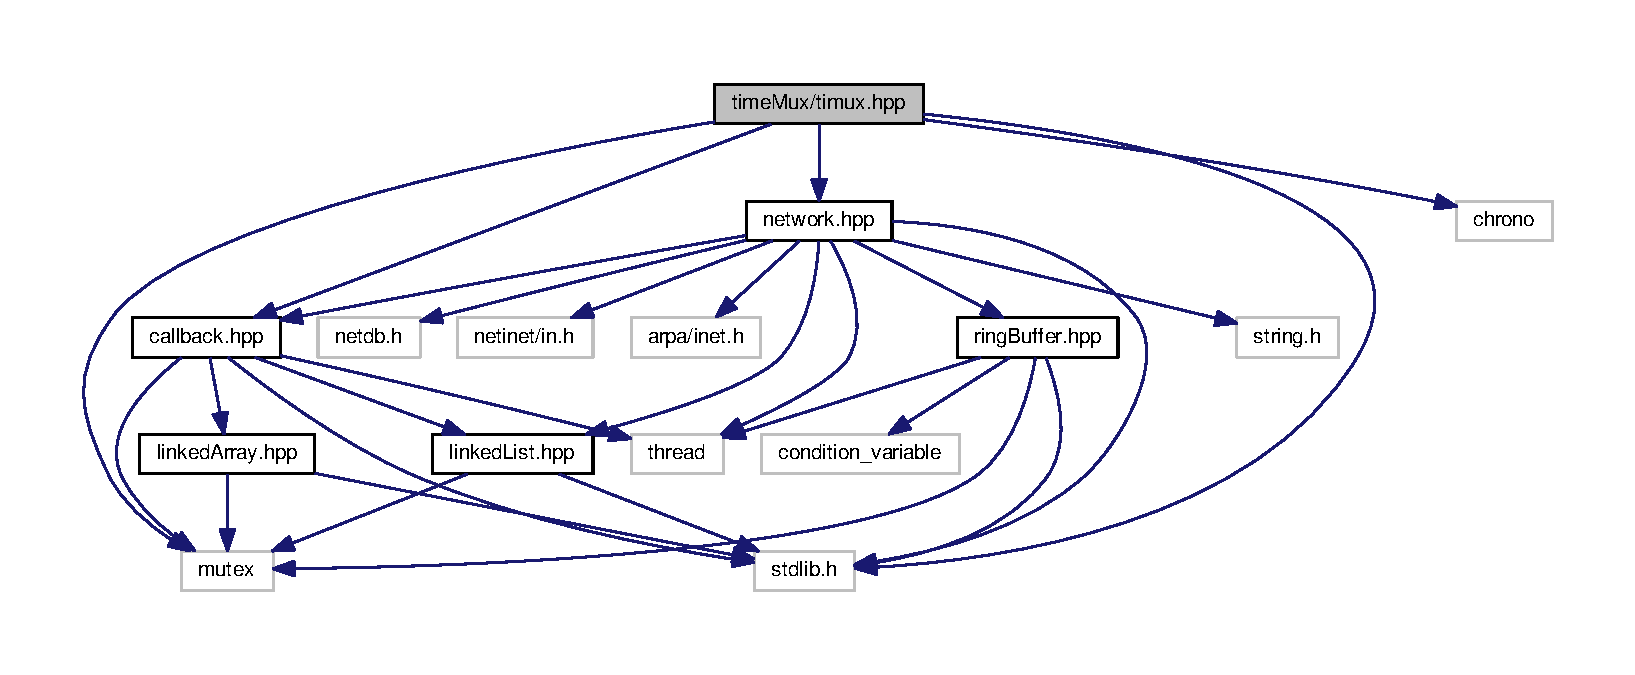
\includegraphics[width=350pt]{timux_8hpp__incl}
\end{center}
\end{figure}
This graph shows which files directly or indirectly include this file\+:
\nopagebreak
\begin{figure}[H]
\begin{center}
\leavevmode
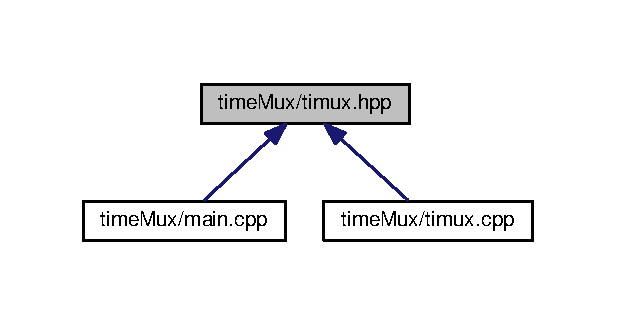
\includegraphics[width=296pt]{timux_8hpp__dep__incl}
\end{center}
\end{figure}
\subsection*{Classes}
\begin{DoxyCompactItemize}
\item 
struct \hyperlink{structtimux_1_1package}{timux\+::package}
\begin{DoxyCompactList}\small\item\em a package as recived from the U\+D\+P socket can be direkly written to \end{DoxyCompactList}\item 
struct \hyperlink{structtimux_1_1msg}{timux\+::msg}
\begin{DoxyCompactList}\small\item\em more user friendly representation of a package does not containn all data, because it is no longer relevant \end{DoxyCompactList}\item 
class \hyperlink{classtimux_1_1timing}{timux\+::timing}
\begin{DoxyCompactList}\small\item\em used for timing and time synchronisation is thread save \end{DoxyCompactList}\item 
class \hyperlink{classtimux_1_1timux}{timux\+::timux}
\begin{DoxyCompactList}\small\item\em the main Class that performess all the logic \end{DoxyCompactList}\end{DoxyCompactItemize}
\subsection*{Namespaces}
\begin{DoxyCompactItemize}
\item 
 \hyperlink{namespacetimux}{timux}
\end{DoxyCompactItemize}
\subsection*{Macros}
\begin{DoxyCompactItemize}
\item 
\#define \hyperlink{timux_8hpp_a1b8511f6591071dfa1f718b1cc1b69e9}{T\+I\+M\+U\+X\+\_\+\+Time\+Signal}~(1)
\item 
\#define \hyperlink{timux_8hpp_ad32d053f7dbac6c922a73695f3a84bce}{T\+I\+M\+U\+X\+\_\+\+Sot\+Signal}~(2)
\item 
\#define \hyperlink{timux_8hpp_add5f72936fed0c9f0a8434b3f4d16be2}{T\+I\+M\+U\+X\+\_\+\+T\+R\+Y\+T\+O\+J\+O\+I\+N}~5
\item 
\#define \hyperlink{timux_8hpp_a3ddd10cae37188220e210c8c1b4acfaa}{T\+I\+M\+U\+X\+\_\+\+T\+R\+Y\+\_\+\+T\+A\+K\+E\+\_\+\+S\+L\+O\+T}~2
\end{DoxyCompactItemize}
\subsection*{Functions}
\begin{DoxyCompactItemize}
\item 
struct \hyperlink{structtimux_1_1package}{timux\+::package} \hyperlink{namespacetimux_a31970845e61d49b6ee9f97328d9aebcc}{timux\+::\+\_\+\+\_\+attribute\+\_\+\+\_\+} ((packed))
\item 
bool \hyperlink{namespacetimux_af9d865eb949c95b170ca458395332f06}{timux\+::\+Time\+Synchronize\+Signal} (\hyperlink{structllu_1_1network_1_1recived_message}{llu\+::network\+::recived\+Message} $\ast$m, \hyperlink{namespacellu_1_1callback_a082ed24306809c4d250bd5ddfbae177f}{llu\+::callback\+::signal} $\ast$s)
\begin{DoxyCompactList}\small\item\em signals a T\+I\+M\+U\+X\+\_\+\+Time\+Signal , if the gven message m is from an A-\/\+Station \end{DoxyCompactList}\item 
void \hyperlink{namespacetimux_aaaa8c2d5485d4108b450aa5edf1e3aa3}{timux\+::\+Time\+Synchronize\+Handler} (void $\ast$timing\+Class, \hyperlink{structllu_1_1network_1_1recived_message}{llu\+::network\+::recived\+Message} $\ast$m)
\begin{DoxyCompactList}\small\item\em adjusts the offset of a timing class \end{DoxyCompactList}\item 
bool \hyperlink{namespacetimux_ad0edf69fd830fa995ad603731acd5a20}{timux\+::\+Msg\+Signal} (\hyperlink{structllu_1_1network_1_1recived_message}{llu\+::network\+::recived\+Message} $\ast$m, \hyperlink{namespacellu_1_1callback_a082ed24306809c4d250bd5ddfbae177f}{llu\+::callback\+::signal} $\ast$s)
\begin{DoxyCompactList}\small\item\em signals a T\+I\+M\+U\+X\+\_\+\+Sot\+Signal if a message is recived \end{DoxyCompactList}\item 
void \hyperlink{namespacetimux_a0325847c7fd72e51034fc14c8547d505}{timux\+::\+Msg\+Handler} (void $\ast$timux\+Class, \hyperlink{structllu_1_1network_1_1recived_message}{llu\+::network\+::recived\+Message} $\ast$m)
\begin{DoxyCompactList}\small\item\em handels an M\+S\+G from the Line \end{DoxyCompactList}\end{DoxyCompactItemize}
\subsection*{Variables}
\begin{DoxyCompactItemize}
\item 
uint8\+\_\+t \hyperlink{timux_8hpp_a3835939f8d204327e497456568a53926}{klasse} \mbox{[}1\mbox{]}
\begin{DoxyCompactList}\small\item\em the class of the Station (A or B) \end{DoxyCompactList}\item 
uint8\+\_\+t \hyperlink{timux_8hpp_ad9c7575237a3a2780e8e6d16e1334982}{data} \mbox{[}24\mbox{]}
\begin{DoxyCompactList}\small\item\em the data payload \end{DoxyCompactList}\item 
uint8\+\_\+t \hyperlink{timux_8hpp_a7f381e6387e6ebf4b714dd55c0100e4c}{next\+Slot} \mbox{[}1\mbox{]}
\begin{DoxyCompactList}\small\item\em the next slot, the clint will send on \end{DoxyCompactList}\item 
uint8\+\_\+t \hyperlink{timux_8hpp_addb651b6286e45373916cc2700efe972}{time} \mbox{[}8\mbox{]}
\begin{DoxyCompactList}\small\item\em the time, the data was send on \end{DoxyCompactList}\item 
struct \hyperlink{structtimux_1_1msg}{timux\+::msg} \hyperlink{namespacetimux_a92131d39983869230f2fb19fb9f654a6}{timux\+::\+\_\+\+\_\+attribute\+\_\+\+\_\+}
\end{DoxyCompactItemize}


\subsection{Macro Definition Documentation}
\hypertarget{timux_8hpp_ad32d053f7dbac6c922a73695f3a84bce}{\index{timux.\+hpp@{timux.\+hpp}!T\+I\+M\+U\+X\+\_\+\+Sot\+Signal@{T\+I\+M\+U\+X\+\_\+\+Sot\+Signal}}
\index{T\+I\+M\+U\+X\+\_\+\+Sot\+Signal@{T\+I\+M\+U\+X\+\_\+\+Sot\+Signal}!timux.\+hpp@{timux.\+hpp}}
\subsubsection[{T\+I\+M\+U\+X\+\_\+\+Sot\+Signal}]{\setlength{\rightskip}{0pt plus 5cm}\#define T\+I\+M\+U\+X\+\_\+\+Sot\+Signal~(2)}}\label{timux_8hpp_ad32d053f7dbac6c922a73695f3a84bce}


Definition at line 14 of file timux.\+hpp.

\hypertarget{timux_8hpp_a1b8511f6591071dfa1f718b1cc1b69e9}{\index{timux.\+hpp@{timux.\+hpp}!T\+I\+M\+U\+X\+\_\+\+Time\+Signal@{T\+I\+M\+U\+X\+\_\+\+Time\+Signal}}
\index{T\+I\+M\+U\+X\+\_\+\+Time\+Signal@{T\+I\+M\+U\+X\+\_\+\+Time\+Signal}!timux.\+hpp@{timux.\+hpp}}
\subsubsection[{T\+I\+M\+U\+X\+\_\+\+Time\+Signal}]{\setlength{\rightskip}{0pt plus 5cm}\#define T\+I\+M\+U\+X\+\_\+\+Time\+Signal~(1)}}\label{timux_8hpp_a1b8511f6591071dfa1f718b1cc1b69e9}


Definition at line 13 of file timux.\+hpp.

\hypertarget{timux_8hpp_a3ddd10cae37188220e210c8c1b4acfaa}{\index{timux.\+hpp@{timux.\+hpp}!T\+I\+M\+U\+X\+\_\+\+T\+R\+Y\+\_\+\+T\+A\+K\+E\+\_\+\+S\+L\+O\+T@{T\+I\+M\+U\+X\+\_\+\+T\+R\+Y\+\_\+\+T\+A\+K\+E\+\_\+\+S\+L\+O\+T}}
\index{T\+I\+M\+U\+X\+\_\+\+T\+R\+Y\+\_\+\+T\+A\+K\+E\+\_\+\+S\+L\+O\+T@{T\+I\+M\+U\+X\+\_\+\+T\+R\+Y\+\_\+\+T\+A\+K\+E\+\_\+\+S\+L\+O\+T}!timux.\+hpp@{timux.\+hpp}}
\subsubsection[{T\+I\+M\+U\+X\+\_\+\+T\+R\+Y\+\_\+\+T\+A\+K\+E\+\_\+\+S\+L\+O\+T}]{\setlength{\rightskip}{0pt plus 5cm}\#define T\+I\+M\+U\+X\+\_\+\+T\+R\+Y\+\_\+\+T\+A\+K\+E\+\_\+\+S\+L\+O\+T~2}}\label{timux_8hpp_a3ddd10cae37188220e210c8c1b4acfaa}


Definition at line 73 of file timux.\+hpp.

\hypertarget{timux_8hpp_add5f72936fed0c9f0a8434b3f4d16be2}{\index{timux.\+hpp@{timux.\+hpp}!T\+I\+M\+U\+X\+\_\+\+T\+R\+Y\+T\+O\+J\+O\+I\+N@{T\+I\+M\+U\+X\+\_\+\+T\+R\+Y\+T\+O\+J\+O\+I\+N}}
\index{T\+I\+M\+U\+X\+\_\+\+T\+R\+Y\+T\+O\+J\+O\+I\+N@{T\+I\+M\+U\+X\+\_\+\+T\+R\+Y\+T\+O\+J\+O\+I\+N}!timux.\+hpp@{timux.\+hpp}}
\subsubsection[{T\+I\+M\+U\+X\+\_\+\+T\+R\+Y\+T\+O\+J\+O\+I\+N}]{\setlength{\rightskip}{0pt plus 5cm}\#define T\+I\+M\+U\+X\+\_\+\+T\+R\+Y\+T\+O\+J\+O\+I\+N~5}}\label{timux_8hpp_add5f72936fed0c9f0a8434b3f4d16be2}


Definition at line 72 of file timux.\+hpp.



\subsection{Variable Documentation}
\hypertarget{timux_8hpp_ad9c7575237a3a2780e8e6d16e1334982}{\index{timux.\+hpp@{timux.\+hpp}!data@{data}}
\index{data@{data}!timux.\+hpp@{timux.\+hpp}}
\subsubsection[{data}]{\setlength{\rightskip}{0pt plus 5cm}uint8\+\_\+t data\mbox{[}24\mbox{]}}}\label{timux_8hpp_ad9c7575237a3a2780e8e6d16e1334982}


the data payload 



Definition at line 196 of file timux.\+hpp.

\hypertarget{timux_8hpp_a3835939f8d204327e497456568a53926}{\index{timux.\+hpp@{timux.\+hpp}!klasse@{klasse}}
\index{klasse@{klasse}!timux.\+hpp@{timux.\+hpp}}
\subsubsection[{klasse}]{\setlength{\rightskip}{0pt plus 5cm}uint8\+\_\+t klasse\mbox{[}1\mbox{]}}}\label{timux_8hpp_a3835939f8d204327e497456568a53926}


the class of the Station (A or B) 



Definition at line 195 of file timux.\+hpp.

\hypertarget{timux_8hpp_a7f381e6387e6ebf4b714dd55c0100e4c}{\index{timux.\+hpp@{timux.\+hpp}!next\+Slot@{next\+Slot}}
\index{next\+Slot@{next\+Slot}!timux.\+hpp@{timux.\+hpp}}
\subsubsection[{next\+Slot}]{\setlength{\rightskip}{0pt plus 5cm}uint8\+\_\+t next\+Slot\mbox{[}1\mbox{]}}}\label{timux_8hpp_a7f381e6387e6ebf4b714dd55c0100e4c}


the next slot, the clint will send on 



Definition at line 197 of file timux.\+hpp.

\hypertarget{timux_8hpp_addb651b6286e45373916cc2700efe972}{\index{timux.\+hpp@{timux.\+hpp}!time@{time}}
\index{time@{time}!timux.\+hpp@{timux.\+hpp}}
\subsubsection[{time}]{\setlength{\rightskip}{0pt plus 5cm}uint8\+\_\+t time\mbox{[}8\mbox{]}}}\label{timux_8hpp_addb651b6286e45373916cc2700efe972}


the time, the data was send on 



Definition at line 198 of file timux.\+hpp.


\hypertarget{udp_8cpp}{\section{time\+Mux/udp.cpp File Reference}
\label{udp_8cpp}\index{time\+Mux/udp.\+cpp@{time\+Mux/udp.\+cpp}}
}


Implementation of a U\+D\+P Connection.  


{\ttfamily \#include \char`\"{}udp.\+hpp\char`\"{}}\\*
{\ttfamily \#include $<$iostream$>$}\\*
Include dependency graph for udp.\+cpp\+:
\nopagebreak
\begin{figure}[H]
\begin{center}
\leavevmode
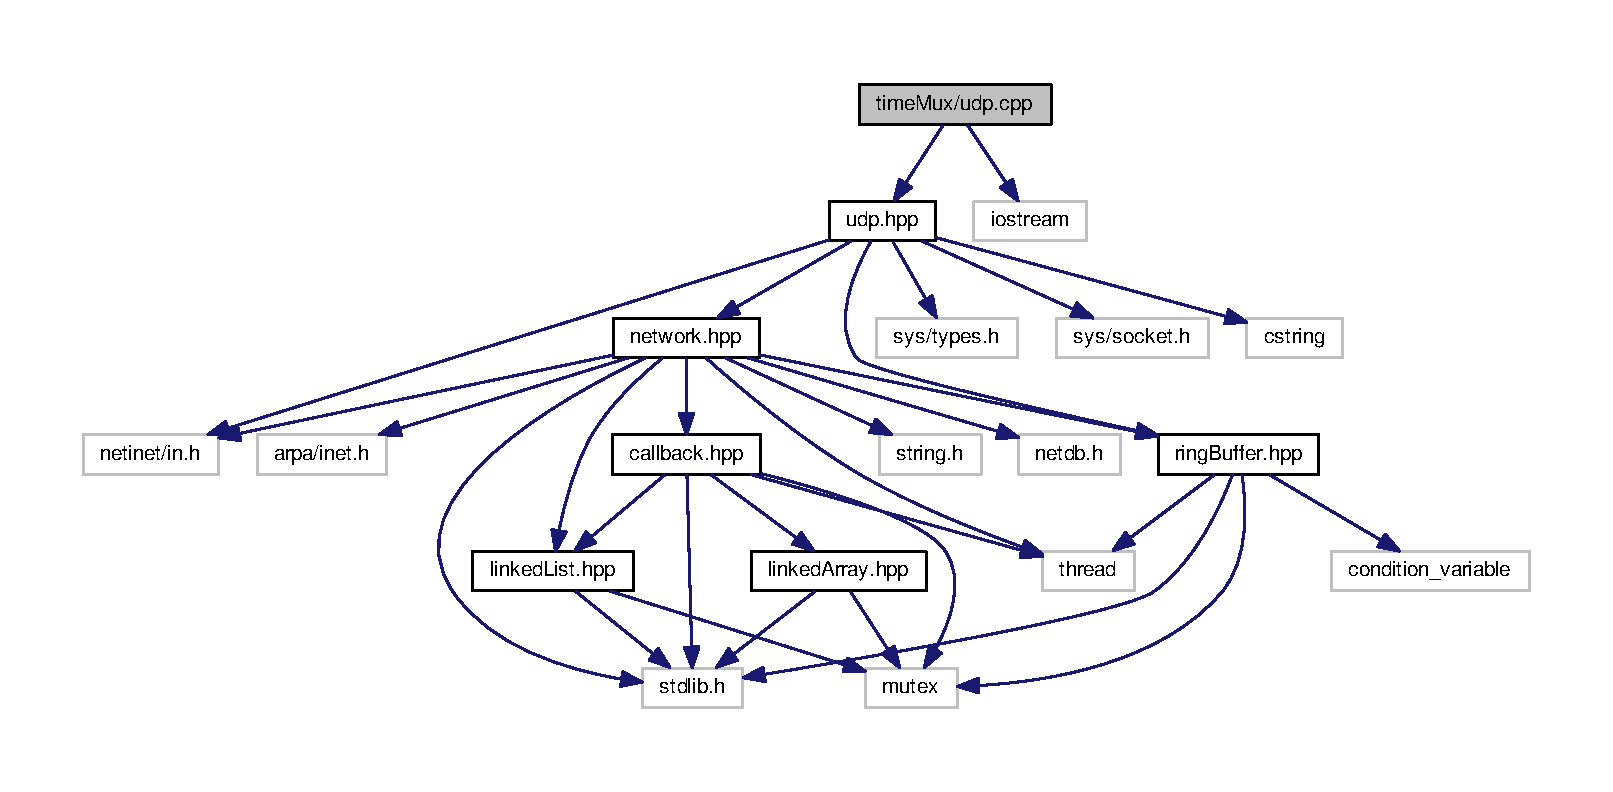
\includegraphics[width=350pt]{udp_8cpp__incl}
\end{center}
\end{figure}
\subsection*{Namespaces}
\begin{DoxyCompactItemize}
\item 
 \hyperlink{namespacellu}{llu}
\item 
 \hyperlink{namespacellu_1_1network}{llu\+::network}
\begin{DoxyCompactList}\small\item\em Contaions functionalety used for network komunikation. \end{DoxyCompactList}\end{DoxyCompactItemize}


\subsection{Detailed Description}
Implementation of a U\+D\+P Connection. 

\begin{DoxyAuthor}{Author}
Lukas Lühr (hexagon2206) 
\end{DoxyAuthor}
\begin{DoxyRefDesc}{Bug}
\item[\hyperlink{bug__bug000010}{Bug}]No known bugs. \end{DoxyRefDesc}


Definition in file \hyperlink{udp_8cpp_source}{udp.\+cpp}.


\hypertarget{udp_8hpp}{\section{time\+Mux/udp.hpp File Reference}
\label{udp_8hpp}\index{time\+Mux/udp.\+hpp@{time\+Mux/udp.\+hpp}}
}


Prototypes for a udp network konnection implementation.  


{\ttfamily \#include $<$netinet/in.\+h$>$}\\*
{\ttfamily \#include $<$sys/types.\+h$>$}\\*
{\ttfamily \#include $<$sys/socket.\+h$>$}\\*
{\ttfamily \#include $<$cstring$>$}\\*
{\ttfamily \#include \char`\"{}network.\+hpp\char`\"{}}\\*
{\ttfamily \#include \char`\"{}ring\+Buffer.\+hpp\char`\"{}}\\*
Include dependency graph for udp.\+hpp\+:
\nopagebreak
\begin{figure}[H]
\begin{center}
\leavevmode
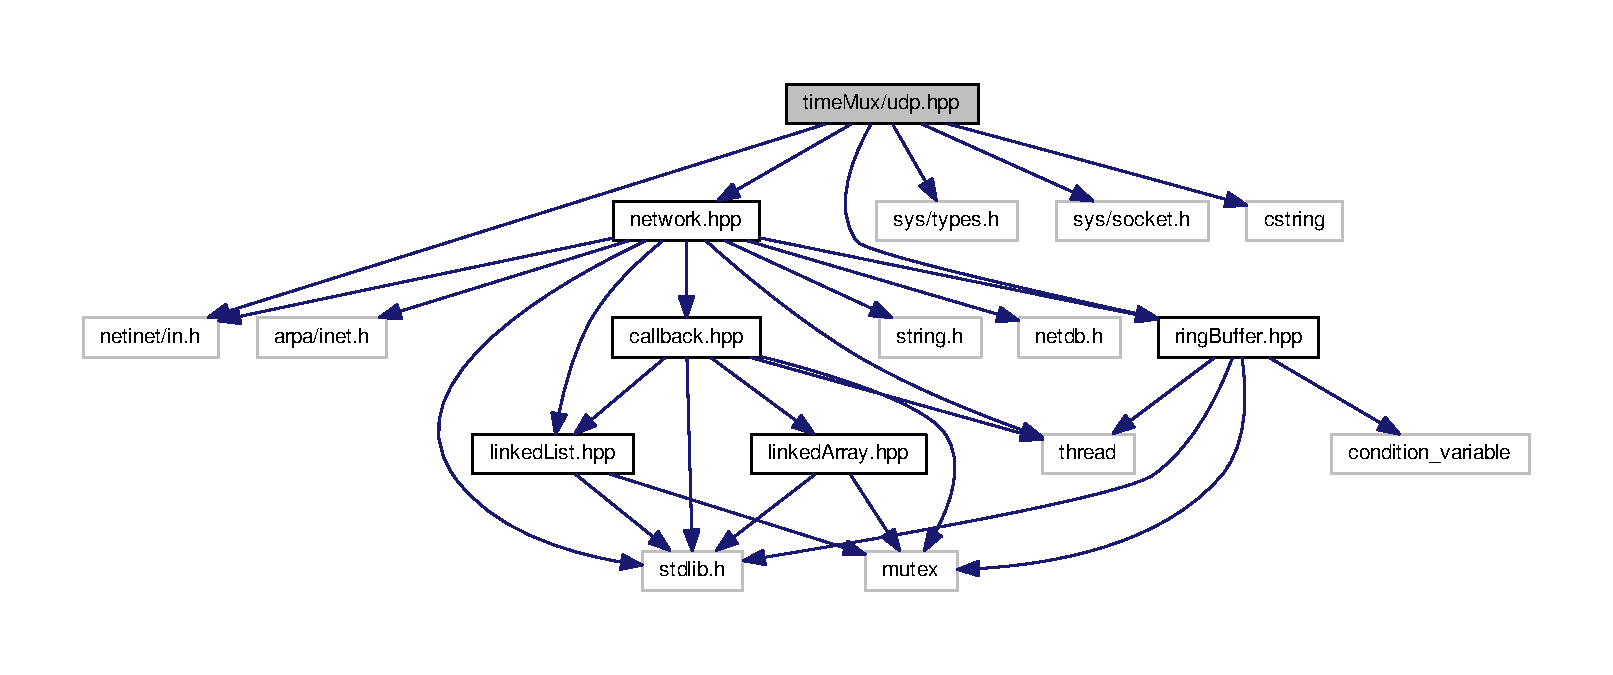
\includegraphics[width=350pt]{udp_8hpp__incl}
\end{center}
\end{figure}
This graph shows which files directly or indirectly include this file\+:
\nopagebreak
\begin{figure}[H]
\begin{center}
\leavevmode
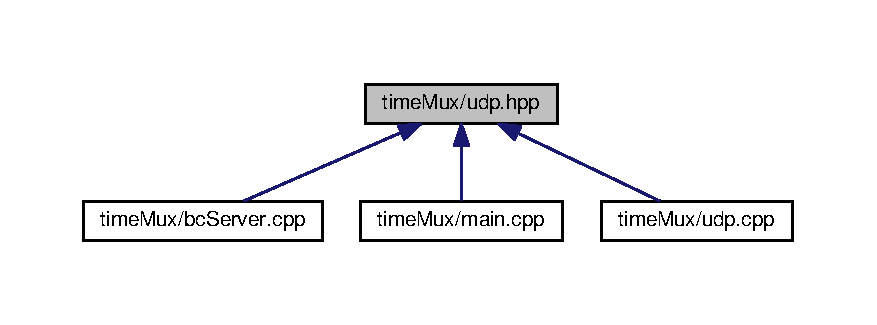
\includegraphics[width=350pt]{udp_8hpp__dep__incl}
\end{center}
\end{figure}
\subsection*{Classes}
\begin{DoxyCompactItemize}
\item 
class \hyperlink{classllu_1_1network_1_1_udp_connection}{llu\+::network\+::\+Udp\+Connection}
\end{DoxyCompactItemize}
\subsection*{Namespaces}
\begin{DoxyCompactItemize}
\item 
 \hyperlink{namespacellu}{llu}
\item 
 \hyperlink{namespacellu_1_1network}{llu\+::network}
\begin{DoxyCompactList}\small\item\em Contaions functionalety used for network komunikation. \end{DoxyCompactList}\end{DoxyCompactItemize}


\subsection{Detailed Description}
Prototypes for a udp network konnection implementation. 

\begin{DoxyAuthor}{Author}
Lukas Lühr (hexagon2206) 
\end{DoxyAuthor}
\begin{DoxyRefDesc}{Bug}
\item[\hyperlink{bug__bug000011}{Bug}]No known bugs. \end{DoxyRefDesc}


Definition in file \hyperlink{udp_8hpp_source}{udp.\+hpp}.


%--- End generated contents ---

% Index
\newpage
\phantomsection
\addcontentsline{toc}{chapter}{Index}
\printindex

\end{document}
